\chapter{\mbox{Probabilistic modelling}}\label{ch:probabilistic-modelling}

%\marginpar{We are hardly able to get through one waking hour without facing some situation (e.g. will it rain or won’t it?) where we do not have enough information to permit deductive reasoning \\--- Edward Jaynes}
\marginpar{The actual science of logic is conversant at present only with things either certain, impossible, or entirely doubtful, none of which (fortunately) we have to reason on. Therefore the true logic for this world is the calculus of probabilities\\---James Clerk Maxwell}
Inference is the process of drawing conclusions from evidence. Much of our lives are spent making inferences about the world given our observations of it; in particular inference is a central aspect of the scientific process. Although deductive logic offers a framework for inferring conclusions from absolute statements of truth, it does not apply to the more typical real-world setting where the information we receive is subject to uncertainty. 

%\marginpar{Probability theory is nothing but common sense reduced to calculation. \\--- Pierre-Simon Laplace}%
To make inferences under conditions of uncertainty, we must instead turn to probability theory. Probabilities offer a consistent framework for quantifying the uncertainty in our beliefs about the world and making inferences given these beliefs. The output of the inference process is itself probabilistic, reflecting that the conclusions we make given uncertain information will themselves be subject to uncertainty. 

%Various axiomatic bases have been proposed for deriving the laws of probability. Of particular note are the Kolmogorov axioms \citep{} which are the basis for the modern measure-theoretic formulation of probability theory. Cox's theorem \citep{} and related work by Polya \citep{} and Jaynes \citep{}, offers an alternative axiomatic basis for deriving probability theory from a minimal set of `common-sense' postulates, with resulting system of \emph{plausible reasoning} seen as natural extension of formal deductive logic under conditions of uncertainty. There has been much philosophical debate over the interpretation of probabilties

%\marginpar{Probability theory is nothing but common sense reduced to calculation. \\--- Pierre-Simon Laplace}
In this chapter we will first introduce the probability notation we will use in the rest of this work, and state some basic results which will be important in the later chapters. We will introduce graphical models as a compact way of visualising structure in probabilistic models. Finally we will give a concrete definition of the inference tasks that the methods presented in the rest of this thesis are aimed at computing (approximate) solutions to,and motivate why such approximate computational methods are needed.

%We will here largely ignore philosophical disucssions of interpretations of probabilities, and instead concentrate on the computational aspects of performing probabilistic inference.

\section{Probability theory}\label{sec:probability-theory}

A \emph{probability space} is defined as a triplet $(\set{S},\,\sset{E},\,\probability)$ where

\begin{itemize}
  \item $\set{S}$ is the \emph{sample space}, the set of all possible outcomes,
  \marginpar{A $\sigma$-algebra, $\sset{E}$, on a set $\set{S}$ is set of subsets of $\set{S}$ with $\set{S} \in \sset{E}$, $\emptyset \in \sset{E}$ and which is closed under complement and countable unions and intersections.}
  \item $\sset{E}$ is the \emph{event space}, a $\sigma$-algebra on $\set{S}$, defining all possible events (measurable subsets of $\set{S}$),
  \item $\probability$ is the \emph{probability measure}, a finite measure satisfying $\probability(\set{S}) = 1$, which specifies the probabilities of events in $\sset{E}$.
\end{itemize}

\marginpar{\raggedright
Kolmogorov's axioms:
  \begin{enumerate}[leftmargin=0pt]
    \item Non-negativity: $\probability(\set{E}) \geq 0 ~\forall \set{E} \in \sset{E}$, 
    \item Normalisation: $\probability(\set{S}) = 1$, 
    \item Countable additivity: for any countable set of disjoint events 
    $\fset{\set{E}_i}_i :$ $\set{E}_i \in \sset{F} ~\forall i$, 
    $\set{E}_i \cap \set{E}_j = \emptyset ~\forall i \neq j$, 
    $\probability\lpa \cup_i \set{E}_i\rpa = \sum_{i} \probability(\set{E}_i)$.
  \end{enumerate}
}
%\marginpar{Kolmogorov's axioms\\1. The probability of an event is real and non-negative. \\2. The probability of the sample space is 1. \\3. The probability of any countable set of mutually exclusive events is equal to the sum of the individual event probabilties.}
Given this definition of a probability space, Kolmogorov's axioms \citep{kolmogorov1950foundations} can be used to derive a measure-theoretic formulation of probability theory. The probability of an event $\set{E} \in \sset{E}$ is defined as its measure $\probability(\set{E})$. Two events $\set{A},\set{B} \in \sset{E}$ are \emph{independent} if $\probability(\set{A}\cap\set{B}) = \probability(\set{A})\probability(\set{B})$.

A measure-theoretic approach has the advantage of providing a unified treatment for describing probabilities on both finite and infinite sample spaces. Although alternative derivations of the laws of probability from different premises such as Cox's theorem \citep{cox1946probability,cox1963algebra} have been proposed, modern extensions of this work result in a calculus of probabilities that is equivalent to Kolmogorov's \citep{terenin2015cox}, with the differences mainly being in the philosophical interpretations of probabilities.

\subsection{Random variables}\label{subsec:random-variables}

\marginpar{If $(\set{X},\,\sset{F})$ and $(\set{Y},\,\sset{G})$ are two measurable spaces, a function $f : \set{X} \to \set{Y}$ is measurable if $f^{-1}(\set{E}) \in \sset{F}$ $\forall \set{E} \in \sset{G}$.}
When modelling real-world processes, rather than considering events as subsets of an abstract sample space, it is usually more helpful to consider \emph{random variables} which represent quantities in the model of interest. A random variable $\rvar{x} : \set{S} \to \set{X}$ is defined as a measurable function from the sample space to a measurable space $(\set{X},\,\sset{F})$. 

\marginpar{The Borel $\sigma$-algebra $\borel(\reals)$ is the smallest $\sigma$-algebra on $\reals$ which contains all open real intervals.}
Often $\set{X}$ is the reals, $\reals$, and $\sset{F}$ is the Borel $\sigma$-algebra on the reals, $\borel(\reals)$, in which case we will refer to a \emph{real random variable}. It is also common to consider cases where $\set{X}$ is a real vector space, $\reals^D$, and $\sset{F} = \borel(\reals^D)$ - in this case we will term the resulting random variable a \emph{random vector} and use the notation $\rvct{x} : \set{S} \to \set{X}$. A final special case is when $\set{X}$ is countable and $\sset{F}$ is the power set $\powerset(\set{X})$ in which case we will refer to $\rvar{x}$ as a \emph{discrete random variable}.

\marginpar{If $(\set{X},\,\sset{F})$ and $(\set{Y},\,\sset{G})$ are two measurable spaces, $\mu$ a measure on these spaces and $f : \set{X} \to \set{Y}$ a measurable function, the pushforward measure $\mu_f$ satisfies $\mu_f(\set{A}) = \mu \circ f^{-1}(\set{A})$ $\forall \set{A} \in \sset{G}$.}
Due to the definition of a random variable as a measurable function, we can define a pushforward measure on a random variable $\rvar{x}$
\begin{equation}
  \prob{\rvar{x}}(A) 
  = \probability\circ\rvar{x}^{-1}(\set{A})
  = \probability\lpa \lbr s \in \set{S}: \rvar{x}(s) \in A \rbr \rpa
  \quad \forall \set{A} \in \sset{F}.
\end{equation}
The measure $\prob{\rvar{x}}$ specifies that the probability of the event that the random variable $\rvar{x}$ takes a value in a measurable set $\set{A} \in \sset{F}$ is $\prob{\rvar{x}}(\set{A})$. We will sometimes describe $\prob{\rvar{x}}$ as the \emph{probability distribution} of $\rvar{x}$.

%Random variables will play a central role in the explanation of the work in this thesis. We will consider a random variable to represent a quantity we are uncertain about the value of; that uncertainty may be considered to arise from incomplete knowledge of the quantity or it having a fundamentally stochastic nature, this is mainly an issue of interpretation which we will largely sidestep.

\subsection{Joint and conditional probability}\label{subsec:joint-and-conditional-probabilities}

Often we will jointly define multiple random variables on the same probability space. Let $(\set{S},\,\sset{E},\,\probability)$ be a probability space and $\rvar{x} : \set{S} \to \set{X}$, $\rvar{y} : \set{S} \to \set{Y}$ be two random variables with corresponding $\sigma$-algebras $\sset{F}$ and $\sset{G}$. Then the \emph{joint probability} of $\rvar{x}$ and $\rvar{y}$ is defined as
\begin{equation}\label{eq:joint-probability-rvar}
  \prob{\rvar{x},\rvar{y}}(\set{A},\,\set{B}) = 
  \probability\lpa \rvar{x}^{-1}(\set{A}) \cap \rvar{y}^{-1}(\set{B})\rpa
  \quad \forall \set{A} \in \sset{F},\,\set{B} \in \sset{G}.
\end{equation}
The joint probability is related to $\prob{\rvar{x}}$ and $\prob{\rvar{y}}$ by
\begin{equation}\label{eq:sum-rule-rvar}
  \prob{\rvar{x},\rvar{y}}(\set{A},\,\set{Y}) =
  \prob{\rvar{x}}(\set{A}),~
  \prob{\rvar{x},\rvar{y}}(\set{X},\,\set{B}) =
  \prob{\rvar{y}}(\set{B})
  \quad \forall \set{A} \in \sset{F},\,\set{B} \in \sset{G}.
\end{equation}
In this context $\prob{\rvar{x}}$ and $\prob{\rvar{y}}$ are referred to as \emph{marginals} of the joint.

The two random variables are said to be independent if and only if
\begin{equation}\label{eq:independent-rvars}
  \prob{\rvar{x},\,\rvar{y}}(\set{A},\set{B}) = \prob{\rvar{x}}(\set{A})\prob{\rvar{y}}(\set{B})
  \quad \forall \set{A} \in \sset{F},\,\set{B} \in \sset{G}.
\end{equation}
\marginpar{In Kolmogorov's probability theory, \eqref{eq:conditional-probability} is given as an additional definition distinct from the basic axioms. In alternatives such as the work of Cox \citep{cox1946probability,cox1963algebra} and de Finetti \citep{de1992foresight}, conditional probabilities are instead viewed as a primitive.}
Also useful is the definition of \emph{conditional probability}
\begin{equation}\label{eq:conditional-probability}
  \probability(\set{A} \gvn \set{B}) =
  \frac{\probability(\set{A} \cap \set{B})}{\probability(\set{B})}
  \quad \forall \set{A} \in \sset{E},\,\set{B} \in \sset{E} : \probability(\set{B}) \neq 0.
\end{equation}
Correspondingly, the conditional probabilities of random variables $\prob{\rvar{x}|\rvar{y}}$ and $\prob{\rvar{x}|\rvar{y}}$ can likewise be defined as satisfying
\begin{equation}\label{eq:product-rule}
\begin{split}
  \prob{\rvar{x},\rvar{y}}(\set{A},\,\set{B}) =
  \prob{\rvar{x}|\rvar{y}}(\set{A} \gvn \set{B}) \, \prob{\rvar{y}}(\set{B}) =
  \prob{\rvar{y}|\rvar{x}}(\set{B} \gvn \set{A}) \, \prob{\rvar{x}}(\set{A})\\
  \forall \set{A} \in \sset{F},\,\set{B} \in \sset{G} : 
  \prob{\rvar{x},\rvar{y}}(\set{A},\,\set{B}) \neq 0,
\end{split}
\end{equation}
which is sometimes referred to as the product rule. 

An implication of \eqref{eq:product-rule} is what is often termed \emph{Bayes' theorem}
\begin{equation}\label{eq:bayes-theorem}
\begin{split}
  \prob{\rvar{x}|\rvar{y}}(\set{A} \gvn \set{B}) =
  \frac
    {\prob{\rvar{y}|\rvar{x}}(\set{B} \gvn \set{A}) \, \prob{\rvar{x}}(\set{A})}
    {\prob{\rvar{y}}(\set{B})} 
  \quad
  \forall \set{A} \in \sset{F},\,
  \set{B} \in \sset{G} : \prob{\rvar{y}}(\set{B}) \neq 0,
\end{split}
\end{equation}
which will be of key importance in the later discussion of inference.

The definition in \eqref{eq:joint-probability-rvar} of the joint probability of a pair of random variables can be extended to arbitarily large collections of random variables. Similarly conditional probabilities can be defined for collections of multiple jointly dependent random variables, with the product rule given in \eqref{eq:product-rule} generalising to a combinatorial number of possible factorisations of the joint probability. Graphical models offer a convenient way of representing the dependencies between large collections of random variables and any resulting factorisation structure in their joint probability, and will be discussed later in this chapter in section \ref{sec:graphical-models} .

\subsection{Probability densities}\label{subsec:probability-densities}

So far we have ignored how the probability measure $\probability$ is defined and by consequence the probability of a random variable. 
\marginpar{A measure on $\set{X}$ is $\sigma$-finite if $\set{X}$ is a countable union of finite measure sets.}
The Radon--Nikodym theorem guarantees that for a pair of $\sigma-$finite measures $\mu$ and $\nu$ on a measurable space $(\set{X},\,\sset{F})$ where $\nu$ is absolutely continuous with respect to $\mu$,  then there is a unique (up to $\mu$-null sets) measurable function $f : \set{X} \to [0,\infty)$ termed a \emph{density} such that
\begin{equation}\label{eq:radon-nikodym}
  \nu(\set{A}) = \int_{\set{A}} f\,\dr\mu
  \quad \forall \set{A} \in \sset{F}.
\end{equation}
\marginpar{If $\mu$ and $\nu$ are measures on a measurable space $(\set{X},\,\sset{F})$ then $\nu$ has absolute continuity \acs{wrt} to $\mu$ if $~\forall \set{A} \in \sset{F}$, \mbox{$\mu(\set{A})=0 \Rightarrow \nu(\set{A})=0$.}}
The density function $f$ is also termed the \emph{Radon-Nikodym derivative} of $\nu$ with respect to $\mu$, denoted $\td{\nu}{\mu}$. Density functions therefore represent a convenient way to define a probability measure with respect to an appropriate base measure. % (which the probability measure will be absolutely continuous with respect to).
It can also be shown that if $f = \td{\nu}{\mu}$ and  $g$ is a 	 measurable function that
\begin{equation}\label{eq:integral-wrt-density}
  \int_{\set{X}} g\,\dr\nu = \int_{\set{X}} g\, f\,\dr\mu,
\end{equation}
which we will use later when discussing calculation of expectations.

%\marginpar{The Lebesgue measure $\lebm{1}(\set{E})$ of a subset $\set{E} \subseteq \reals$ is $\lebm{1}(\set{E}) = \inf\lbrace \sum_{i=1}^\infty (b_i - a_i) :$ $E \subseteq \cup_{i=1}^\infty [a_i,\,b_i],$ $a_i,b_i \in \reals, a_i \leq b_i ~\forall i\in\naturals\rbrace$.}
For real random variables, an appropriate base measure is the \emph{Lebesgue measure}, $\lebm{1}$, on $\reals$. The probability $\prob{\rvar{x}}$ of a real random variable $\rvar{x}$ can then be defined via a \emph{probability density} $\pden{\rvar{x}} : \reals \to [0,\,\infty)$ by
\begin{equation}\label{eq:real-rv-prob-dens}
    \prob{\rvar{x}}(\set{A})
    = \int_{\set{A}} \pden{\rvar{x}} \,\dr\lebm{1}
    = \int_{\set{A}} \pden{\rvar{x}}(x) \,\dr x
    \qquad
    \forall \set{A} \in \borel(\reals).
\end{equation}
Analagously for a random vector $\rvct{x}$ with density $\pden{\rvct{x}} : \reals^D \to [0,\,\infty)$ with respect to the $D$-dimensional Lebesgue measure $\lebm{D}$
\begin{equation}\label{eq:vector-prob-dens}
    \prob{\rvct{x}}(\set{A})
    = \int_{\set{A}} \pden{\rvct{x}} \,\dr\lebm{D}
    = \int_{\set{A}} \pden{\rvct{x}}(\vct{x}) \,\dr \vct{x}
    \qquad
    \forall \set{A} \in \borel(\reals^D).
\end{equation}
%The normalisation requirement for the probability measure $\probability_{\rvar{x}}$ means that $\int_{\set{X}}\pden{\rvar{x}}\,\dr\lebm{1} = 1$. 
The notation in the second equalities in \eqref{eq:real-rv-prob-dens} and \eqref{eq:vector-prob-dens} uses a convention that will be used throughout this thesis that integrals without an explicit measure are with respect to the Lebesgue measure. 
\marginpar{The counting measure $\countm$ is defined as $\countm(\set{A}) = |\set{A}|$ for all finite $\set{A}$ and $\countm(\set{A}) = +\infty$ otherwise.}

For discrete random variables, an appropriate base measure is instead \pagebreak the \emph{counting measure}, $\countm$. The probability of a discrete random variable is then defined via a probability density $\pden{\rvar{x}} : \set{X} \to [0,\,1]$ by
\begin{equation}
    \prob{\rvar{x}}(\set{A})
    = \int_{\set{A}} \pden{\rvar{x}} \,\dr\countm
    = \sum_{x \in \set{A}} \pden{\rvar{x}}(x) 
    \qquad
    \forall \set{A} \in \powerset(\set{X}).
\end{equation}
The co-domain of a probability density $\pden{\rvar{x}}$ for a discrete random variable is restricted to $[0,\,1]$ due to the non-negativity and normalisation requirements for the probability measure $\prob{\rvar{x}}$, with $\sum_{x\in\set{X}} \pden{\rvar{x}}(x) = 1$. Commonly for the case of a discrete random variable, the density $\pden{\rvar{x}}$ is instead referred to as a \emph{probability mass function}, with density reserved for real random variables. We will however use \emph{probability density} in both cases in keeping with the earlier definition of a density with respect to a base measure, this avoiding difficulties when definining joint probabilities on a mixture of real and discrete random variables.

The joint probability $\prob{\rvar{x},\rvar{y}}$ of a pair of random variables $\rvar{x}$ and $\rvar{y}$ with co-domains the measurable spaces $(\set{X},\,\sset{F})$ and $(\set{Y},\,\sset{G})$ respectively, can be defined via a joint probability density $\pden{\rvar{x},\rvar{y}} : \set{X} \times \set{Y} \to [0,\infty)$ by
\begin{equation}\label{eq:real-rv-joint-prob-dens}
  \prob{\rvar{x},\rvar{y}}(\set{A},\set{B}) =
  \int_{\set{A}\times\set{B}} 
    \pden{\rvar{x},\rvar{y}} 
  \,\dr(\mu_{\rvar{x}} \times \mu_{\rvar{y}})
  \quad \forall \set{A} \in \sset{F}, \,\set{B} \in \sset{G},
\end{equation}
\marginpar{If $(\set{X}_1,\,\sset{F}_1,\,\mu_1)$ and $(\set{X}_2,\,\sset{F}_2,\,\mu_2)$ are two measure spaces, the product measure $\mu_1 \times \mu_2$ on a measurable space $(\set{X}_1\times\set{X}_2,\,\sset{F}_1\otimes\sset{F}_2)$ is defined as satisfying $(\mu_1\times\mu_2)(\set{A}_1\times\set{A}_2) = \mu_1(\set{A}_1)\mu_2(\set{A}_2)$ $\forall \set{A}_1\in\sset{F}_1,\,\set{A}_2\in\sset{F}_2$.}
where $\mu_{\rvar{x}} \times \mu_{\rvar{y}}$ represents the product measure of two appropriate base measures $\mu_{\rvar{x}}$ and $\mu_{\rvar{y}}$, e.g. $\mu_{\rvar{x}} = \lebm{1}$ and $\mu_{\rvar{y}} = \countm$ if $\rvar{x}$ is a real random variable and $\rvar{y}$ is a discrete random variable.

When dealing with random variables, we will often only specify the co-domain of the random variable(s) and a (joint) probability density, with the base measure being implicitly defined as the Lebesgue measure for real random variables (or vectors), counting measure for discrete random variables and an appropriate product measure for a mix of random variables. Similarly we will usually neglect to explicitly define the probability space $(\set{S},\,\sset{E},\,\probability)$ which the random variable(s) map from. In this case we will typically use the loose notation $\rvar{x} \in \set{X}$ to mean a random variable $\rvar{x}$ with co-domain $\set{X}$. 

This less explicit but more succinct probability notation in terms of random variables and densities is common in the machine learning and computational statitistics literature and will generally be preferred to improve readability. 
%The underlying measure-theoretic basis of these concepts will however be important for some of the upcoming definitions in this chapter and some of the derivations later in the thesis. 
Tables \ref{tab:standard-distributions-discrete}, \ref{tab:standard-distributions-unbounded} and \ref{tab:standard-distributions-bounded} give definitions of the densities and shorthand notation for some common parametric probability distributions that we will use in this thesis.

\newgeometry{
  includehead,
  includemp,
  headsep=5mm,
  %nomarginpar,
  marginparsep=8mm,
  marginparwidth=27mm,	
  top=20mm,
  bottom=40mm,
  outer=20mm,
  inner=40mm
}

\begin{landscape}
\vspace*{-8mm}
\begin{table}[H]
\centering
\begin{tabular}{p{4cm}p{5cm}lll}
\toprule
  \textsf{Name} & \textsf{Parameters} & \textsf{Shorthand} & \textsf{Density} & Support \\
\midrule
%%%%%%%%%%%%%
  Bernoulli & 
  $\pi \in [0,1]$ &
  $\textrm{Ber}(x \gvn \pi)$ & 
  $\pi^x (1 -\pi)^{(1-x)}$ &
  $x \in \fset{0,1}$\\
%%%%%%%%%%%%%
  Categorical & 
  $\vct{\pi} \in \vvmathbb{S}^K$ &
  $\textrm{Cat}(x \gvn \vct{\pi})$ & 
  $\sum_{k=1}^K \lpa \ind{\fset{k}}(x) \pi_k \rpa$ &
  $x \in \fset{1 \dots K}$\\
%%%%%%%%%%%%%
\bottomrule
\end{tabular}
\caption[Standard discrete density definitions.]{Definitions of densities of parameteric distributions for discrete random variables that will be used in this thesis.}
\label{tab:standard-distributions-discrete}
\end{table}

\begin{table}[H]
\centering
\begin{tabular}{p{4cm}p{5cm}ll}
\toprule
  \textsf{Name} & \textsf{Parameters} & \textsf{Shorthand} & \textsf{Density} \\
\midrule
%%%%%%%%%%%%%
  Normal & 
  \setlength\tabcolsep{0pt}
  \begin{tabular}{ll}
  $\mu \in \reals$ &~: mean\\[-1mm]
  $\sigma > 0$ &~: standard deviation 
  \end{tabular} &
  $\nrm{x \gvn \mu,\sigma^2}$ & 
  $\frac{1}{\sqrt{2\uppi}\sigma} \exp\lpa -\frac{(x-\mu)^2}{2\sigma^2}\rpa$ \\[0mm]
%%%%%%%%%%%%%
  Multivariate normal &
  \setlength\tabcolsep{0pt}
  \begin{tabular}{ll}
  $\vct{\mu} \in \reals^D$ &~: mean vector \\[-1mm]
$\mtx{\Sigma} \in \sset{S}^{D}_{++}$ &~: covariance matrix
  \end{tabular} &
  $\nrm{\vct{x} \gvn \vct{\mu}, \mtx{\Sigma}}$ & 
  $\frac{1}{\sqrt{(2\uppi)^D|\mtx{\Sigma}|}} \exp\lpa -\frac{1}{2} (\vct{x}-\vct{\mu})\tr\mtx{\Sigma}^{-1}(\vct{x}-\vct{\mu})\rpa$ \\[4mm]
%%%%%%%%%%%%%
  Student's \emph{t} & 
  \setlength\tabcolsep{0pt}
  \begin{tabular}{ll}
  $\nu > 0$ &~: degrees of freedom\\[-1mm]
  $\mu \in \reals$ &~: location\\[-1mm]
  $\sigma > 0$ &~: scale\\ 
  \end{tabular} &
  $\mathrm{StT}(x \gvn \nu, \mu, \sigma)$ & 
  $\frac{\upGamma\lpa\frac{\nu + 1}{2}\rpa}{\upGamma\lpa\frac{\nu}{2}\rpa\sqrt{\uppi\nu}\sigma}\lpa 1 + \frac{1}{\nu}\lpa\frac{x-\mu}{\sigma}\rpa^2\rpa^{-\frac{\nu + 1}{2}}$\\[6mm] 
%%%%%%%%%%%%%
%  Cauchy & 
%  \setlength\tabcolsep{0pt}
%  \begin{tabular}{ll}
%  $\mu \in \reals$ &~: location\\
%  $\sigma > 0$ &~: scale 
%  \end{tabular} &
%  $\mathcal{C}(x \gvn \mu, \sigma)$ & 
%  $\frac{1}{\uppi \sigma \lsb 1 + \lpa\frac{x - \mu}{\sigma}\rpa^2\rsb}$ \\[0mm]
%%%%%%%%%%%%%
  Logistic &
  \setlength\tabcolsep{0pt}
  \begin{tabular}{ll}
  $\mu \in \reals$ &~: location\\[-1mm]
  $\sigma > 0$ &~: scale 
  \end{tabular} &
  $\textrm{Logistic}(x \gvn \mu,\sigma)$ & 
  $\frac{1}{4\sigma}\cosh\lpa\frac{x - \mu}{2\sigma}\rpa^{-2}$ \\[0mm]
%%%%%%%%%%%%%
  Inverse cosh  & 
  \setlength\tabcolsep{0pt}
  \begin{tabular}{ll}
  $\mu \in \reals$ &~: location\\[-1mm]
  $\sigma > 0$ &~: scale 
  \end{tabular} &
  $\textrm{InvCosh}(x \gvn \mu, \sigma)$ & 
  $\frac{1}{2\sigma} \cosh\lpa\frac{\uppi(x - \mu)}{2 \sigma}\rpa^{-1}$ \\
%%%%%%%%%%%%%
\bottomrule
\end{tabular}
\caption[Standard unbounded density definitions.]{Definitions of densities of parameteric distributions for unbounded real random variables that will be used in this thesis.}
\label{tab:standard-distributions-unbounded}
\end{table}
\end{landscape}

\begin{landscape}
\begin{table}[htp]
\centering
\begin{tabular}{p{4cm}p{5cm}lll}
\toprule
  \textsf{Name} & \textsf{Parameters} & \textsf{Shorthand} & \textsf{Density} & \textsf{Support} \\
\midrule
%%%%%%%%%%%%%
  Log-normal & 
  \setlength\tabcolsep{0pt}
  \begin{tabular}{ll}
  $\mu \in \reals$ &~: log mean\\[-1mm]
  $\sigma > 0$ &~: log standard deviation 
  \end{tabular} &
  $\textrm{LogNorm}(x \gvn \mu,\sigma^2)$ & 
  $\frac{1}{x\sqrt{2\uppi}\sigma} \exp\lpa -\frac{(\log x-\mu)^2}{2\sigma^2}\rpa$ & 
  $x > 0$ \\[3mm]
%%%%%%%%%%%%%
  Multivariate log-normal &
  \setlength\tabcolsep{0pt}
  \begin{tabular}{ll}
  $\vct{\mu} \in \reals^D$ &~: log mean \\[-1mm]
  $\mtx{\Sigma} \in \sset{S}^{D}_{++}$ &~: log covariance
  \end{tabular} &
  $\textrm{LogNorm}(\vct{x} \gvn \vct{\mu}, \mtx{\Sigma})$ & 
  $\frac{\exp\lpa -\frac{1}{2} (\log\vct{x}-\vct{\mu})\tr\mtx{\Sigma}^{-1}(\log\vct{x}-\vct{\mu})\rpa}{\prod_{d=1}^D(x_d)\sqrt{(2\uppi)^D|\mtx{\Sigma}|}} $ & $\vct{x} \in [0, \infty)^D$ \\[3mm]
%%%%%%%%%%%%%
  Exponential & 
  $\lambda > 0$ : rate &
  $\mathrm{Exp}(x \gvn \lambda)$ & 
  $\lambda \exp(-\lambda x)$ & 
  $x \geq 0$\\[2mm]
%%%%%%%%%%%%%
  Uniform & 
  \setlength\tabcolsep{0pt}
  \begin{tabular}{ll}
  $a \in \reals$ &~: minimum\\[-1mm]
  $b \in \reals$ &~: maximum, $b > a$
  \end{tabular} &
  $\mathcal{U}(x \gvn a, b)$ & 
  $\frac{1}{b-a}\ind{[a,b]}(x)$ & 
  $a \leq x \leq b$\\[3mm]
%%%%%%%%%%%%%
  Half-Cauchy & 
  $\gamma > 0$ : scale &
  $\mathcal{C}_{\geq 0}(x \gvn \gamma)$ & 
  $\frac{2}{\uppi \gamma} \lpa 1 + \frac{x^2}{\gamma^2} \rpa^{-1}$ & 
  $x \geq 0$ \\[2mm]
%%%%%%%%%%%%%
%  Chi-squared & 
%  $k \in \naturals_{+}$ : degrees of freedom &
%  $\chi^2(x \gvn k)$ & 
%  $\frac{x^{\frac{k}{2}-1}\exp\lpa -\frac{x}{2}\rpa}{\Gamma\lpa\frac{k}{2}\rpa 2^{\frac{k}{2}}}$ & 
%  $x > 0$ \\[2mm]
%%%%%%%%%%%%%
  Gamma &
  \setlength\tabcolsep{0pt}
  \begin{tabular}{ll}
  $\alpha > 0$ &~: shape\\[-1mm]
  $\beta > 0$ &~: rate 
  \end{tabular} &
  $\textrm{Gamma}(x \gvn \alpha, \beta)$ & 
  $\frac{\beta^\alpha}{\upGamma(\alpha)} x^{\alpha - 1} \exp(-\beta x)$& 
  $x \geq 0$ \\[3mm]
%%%%%%%%%%%%%
  Beta &
  \setlength\tabcolsep{0pt}
  \begin{tabular}{ll}
  $\alpha > 0$ &~: shape\\[-1mm]
  $\beta > 0$ &~: shape 
  \end{tabular} &
  $\textrm{Beta}(x \gvn \alpha, \beta)$ & 
  $\frac{\upGamma(\alpha + \beta)}{\upGamma(\alpha)\upGamma(\beta)} x^{\alpha - 1} (1 - x)^{\beta - 1}$& 
  $0 \leq x \leq 1$ \\[3mm]
%%%%%%%%%%%%%
  Dirichlet &
  $\vct{\alpha} \in (0,\infty)^K$ : concentration &
  $\textrm{Dir}(\vct{x} \gvn \vct{\alpha})$ & 
  $\frac{\upGamma\lpa \sum_{k=1}^K \alpha_k \rpa}{\prod_{k=1}^K \upGamma(\alpha_k)} \prod_{k=1}^K x_i^{\alpha_k -1}$& 
  $\vct{x} \in \vvmathbb{S}^K$ \\[2mm]
%%%%%%%%%%%%%
  Lomax &
  \setlength\tabcolsep{0pt}
  \begin{tabular}{ll}
  $\alpha > 0$ &~: shape\\[-1mm]
  $\beta > 0$ &~: scale 
  \end{tabular} &
  $\textrm{Lomax}(x \gvn \alpha, \beta)$ & 
  $\frac{\alpha\beta^\alpha}{(\beta + x)^{\alpha + 1}}$& 
  $x \geq 0$ \\
\bottomrule
\end{tabular}
\caption[Standard bounded density definitions.]{Definitions of densities of parameteric distributions for bounded real random variables that will be used in this thesis.}
\label{tab:standard-distributions-bounded}
\end{table}
\end{landscape}
\restoregeometry

\subsection{Transforms of random variables}\label{subsec:change-of-variables}

It is common to define a random variable via a transform of another. Let $\rvar{x}$ be a random variable with co-domain the measurable space $(\set{X},\,\sset{F})$. Further let $(\set{Y},\,\sset{G})$ be a second measurable space and $\phi : \set{X} \to \set{Y}$ a measurable function between the two spaces. If we define $\rvar{y} = \phi \circ \rvar{x}$ then analagously to our original definition of $\prob{\rvar{x}}$ as the pushforward measure of $\probability$ under the measurable function defining $\rvar{x}$, we can define $\prob{\rvar{y}}$ in terms of $\prob{\rvar{x}}$ as
\begin{equation}\label{eq:change-of-variables-probability}
  \prob{\rvar{y}}(\set{A}) = 
  \prob{\rvar{x}} \circ \phi^{-1}(\set{A}) =
  \prob{\rvar{x}}\lpa \lbrace x \in \set{X} : \phi(x) \in \set{A} \rbrace \rpa
  \quad \forall \set{A} \in \sset{G},
\end{equation}
i.e. the probability of the event $\rvar{y} \in \set{A}$ is equal to the probability of $\rvar{x}$ being in the pre-image under $\phi$ of $\set{A}$. To calculate probabilities of transformed random variables therefore we will therefore need to be able to find the pre-images of values of the transformed  variable.

If the probability $\prob{\rvar{x}}$ is defined by a probability density $\pden{\rvar{x}}$ with respect to a measure $\mu_{\rvar{x}}$, we can also in some cases find a density $\pden{\rvar{y}}$ on the transformed variable $\rvar{y} = \phi(\rvar{x})$ with respect to a (potentially different) measure $\mu_{\rvar{y}}$ which can be used to calculate the probability $\prob{\rvar{y}}$, 
\begin{equation}\label{eq:change-of-variables-general}
  \prob{\rvar{y}}(\set{A}) =
  \int_{\phi^{-1}(\set{A})} \pden{\rvar{x}} \,\dr\mu_{\rvar{x}} = 
  \int_{\set{A}} \pden{\rvar{y}} \,\dr\mu_{\rvar{y}}
  \quad \forall \set{A} \in \sset{G}.
\end{equation}

For random variables with countable co-domains where the integral in \eqref{eq:change-of-variables-general} corresponds to a sum, a $\pden{\rvar{y}}$ satisfying \eqref{eq:change-of-variables-general} is simple to identify. If $\rvar{x}$ is a discrete random variable with probability density $\pden{\rvar{x}}$ with respect to the counting measure, then $\rvar{y} = \phi(\rvar{x})$ will necessarily also be a discrete random variable. Applying \eqref{eq:change-of-variables-general} for $\pden{\rvar{x}} = \td{\prob{\rvar{x}}}{\countm}$ we have that
\begin{align}\label{eq:change-of-variables-discrete-derivation}
  \int_{\phi^{-1}(\set{A})} \pden{\rvar{x}}(x) \,\dr\countm(x) &= 
  \sum_{x\in\phi^{-1}(\set{A})} \pden{\rvar{x}}(x)  =
  \sum_{y \in \set{A}} \sum_{x\in\phi^{-1}(y)} \pden{\rvar{x}}(x) \nonumber \\
  &= \int_{\set{A}} \sum_{x\in\phi^{-1}(y)} \pden{\rvar{x}}(x) \,\dr\countm(y)
  \quad \forall \set{A} \in \sset{G}.
\end{align}
We can therefore define $\pden{\rvar{y}} = \td{\prob{\rvar{y}}}{\countm}$ in terms of $\pden{\rvar{x}}$ as
\begin{equation}\label{eq:change-of-variables-discrete}
  \pden{\rvar{y}}(y) = \sum_{x \in \phi^{-1}(y)} \pden{\rvar{x}}(x)
  \quad \forall y \in \set{Y}.
\end{equation}
In the special case that $\phi$ is bijective we have that 
\begin{equation}\label{eq:change-of-variables-discrete-bijective}
  \pden{\rvar{y}}(y) = \pden{\rvar{x}}\circ\phi^{-1}(y)
  \quad \forall y \in \set{Y}.
\end{equation}
For transformations of real random variables and vectors, the situation is more complicated as we need to account for any local contraction or expansion of space by the map $\phi$. Let $\set{X} = \reals^M$ and $\set{Y} = \reals^N$ with $N \leq M, \, N,M \in \naturals$. %(we do not consider the case $N > M$ as would necessarily correspond to the transformed random variable only having support on a $N$ dimensional manifold in $\set{Y}$). 
We will need a result from geometric measure theory, the \emph{co-area formula} \citep{federer1969geometric}. Let $g$ be an $L^1$ integrable function and $\vct{\phi} : \set{X} \to \set{Y}$ a Lipschitz map. Then the co-area formula states that
\begin{equation}\label{eq:co-area-formula}
  \int_{\set{X}} 
    g(\vct{x}) \, J_{\vct{\phi}}(\vct{x})
  \,\dr\lambda^{M}(\vct{x}) =
  \int_{\set{Y}} \int_{\vct{\phi}^{-1}(\vct{y})}
    g(\vct{x})
  \,\dr\haum{M-N}(\vct{x})\,\dr\lebm{N}(\vct{y})
\end{equation}
\marginpar{The $D$-dimensional Hausdorff measure $\haum{D}$ on $\reals^N$ for $D \in \naturals$, $0 < D < N$ formalises a measure of the `volume' of $D$-dimensional submanifolds of $\reals^N$ - e.g. for $D=1$ it corresponds to the length of a curve in $\reals^N$. Additionally $\haum{N} = \lebm{N}$ and $\haum{0} = \countm$.}
where $\haum{D}$ is the $D$-dimensional \emph{Hausdorff measure}  and $J_{\vct{\phi}} : \set{X} \to [0,\infty)$ is the \emph{Jacobian determinant} defined as
\begin{equation}\label{eq:jacobian-determinant-def}
 J_{\vct{\phi}}(\vct{x}) = 
 \left|\pd{\vct{\phi}}{\vct{x}}\pd{\vct{\phi}}{\vct{x}}\tr\right|^{\frac{1}{2}}
 \quad \forall \vct{x} \in \set{X}.
\end{equation}
Now let $\rvct{x}$ be a random vector with co-domain the measurable space $(\set{X},\,\borel(\reals^M))$ and define $\rvct{y} = \vct{\phi} \circ \rvct{x}$ as a random vector with co-domain the measurable space $(\set{Y},\,\borel(\reals^N))$ with $\vct{\phi} : \set{X} \to \set{Y}$ a Lipschitz map as above. Let $\set{Z} = \lbr \vct{x} \in \set{X} : J_{\vct{\phi}}(\vct{x}) = 0 \rbr$ and require that $\prob{\rvar{x}}(\set{Z}) = 0$. Then for $\set{A} \in \borel(\reals^N)$ define an $L^1$ integrable function $g$ as
\begin{equation}\label{eq:change-of-var-real-vector-derivation-1}
  g(\vct{x}) = 
  \begin{cases}
    \ind{\set{A}}\circ\,\vct{\phi}(\vct{x}) \, \pden{\rvct{x}}(\vct{x}) \, J_{\vct{\phi}}(\vct{x})^{-1}
    & \quad \forall \vct{x} \in \set{X} \setminus \set{Z}\\
    0 & \quad \forall \vct{x} \in \set{Z}
  \end{cases}.
\end{equation}
Integrating $g(\vct{x})\,J_{\vct{\phi}}(\vct{x})$ over $\vct{x} \in \set{X}$ we have that
\begin{align}\label{eq:change-of-var-real-vector-derivation-2}
  \int_{\set{X}} 
    g(\vct{x}) \, J_{\vct{\phi}}(\vct{x})
  \,\dr\lambda^{M}(\vct{x}) 
  &=
  \int_{\set{X}\setminus{\set{Z}}}
    \ind{\set{A}}\circ\,\vct{\phi}(\vct{x})\,
    \pden{\rvct{x}}(\vct{x})
  \,\dr\lambda^{M}(\vct{x})\\
  &=
  \int_{\set{X}}
    \ind{\set{A}}\circ\,\vct{\phi}(\vct{x})
  \,\dr\prob{\rvar{x}}(\vct{x})
  \\
  &=
  \int_{\phi^{-1}(\set{A})}
  \,\dr\prob{\rvar{x}}(\vct{x}) = \prob{\rvar{y}}(\set{A}).
\end{align}
The equality between first and second lines comes from the requirement $\prob{\rvar{x}}(\set{Z}) = 0$, with the Lebesgue integrals of a function over two sets which differ by only a zero-measure set equal. Now applying the co-area formula \eqref{eq:co-area-formula} to the left-hand side gives
\begin{equation}\label{eq:change-of-var-real-vector-derivation-3}
  \int_{\set{Y}} \int_{\vct{\phi}^{-1}(\vct{y})} g(\vct{x}) \,\dr\haum{M-N}(\vct{x})\,\dr\lebm{N}(\vct{y})
  = \prob{\rvar{y}}(\set{A}).
\end{equation}
Therefore we can define a density $\pden{\rvar{y}} = \td{\prob{\rvar{y}}}{\lebm{N}}$ satisfying \eqref{eq:change-of-variables-general} as
\begin{equation}\label{eq:change-of-variables-vector}
  \pden{\rvct{y}}(\vct{y}) = 
  \int_{\vct{\phi}^{-1}(\vct{y})} 
    \pden{\rvct{x}}(\vct{x})\,J_{\vct{\phi}}(\vct{x})^{-1}
  \,\dr\haum{M-N}(\vct{x})
  \quad \forall \vct{y} \not\in \vct{\phi}(\set{Z}).
\end{equation}
For the special case of a dimension-preserving map $\vct{\phi}$ with $N = M$ the integral in \eqref{eq:change-of-variables-vector} is with respect to $\haum{0}$ which is equivalent to the counting measure $\countm$. In this case $J_{\vct{\phi}}(\vct{x}) = \left|\pd{\vct{\phi}}{\vct{x}}\right|$ and we therefore get
\begin{equation}\label{eq:change-of-variables-vector-same-dim}
  \pden{\rvct{y}}(\vct{y}) = 
  \sum_{\vct{x} \in \vct{\phi}^{-1}(\vct{y})} 
    \pden{\rvct{x}}(\vct{x}) \, \left| \pd{\vct{\phi}}{\vct{x}} \right|^{-1}
  \quad \forall \vct{y} \not\in \vct{\phi}(\set{Z}).
\end{equation}
Under the further restriction that $\vct{\phi}$ is bi-Lipschitz, i.e. it is bijective and Lipschitz in both directions, we recover the more commonly presented multidimensional change of variables formula
\begin{equation}\label{eq:change-of-variables-vector-bijective}
  \pden{\rvct{y}}(\vct{y}) = 
    \pden{\rvct{x}}\circ\vct{\phi}^{-1}(\vct{y})
    \left|\pd{\vct{\phi}^{-1}}{\vct{y}}\right|
  \quad \forall \vct{y} \in \set{Y}.
\end{equation}
In both of the cases considered, we have seen that if the function $\phi$ the random variable $\rvar{x}$ is mapped through is bijective, the resulting expression for the density on the mapped random variable $\rvar{y}$ is simpler in the sense that the pre-image $\phi^{-1}(y)$ of a point $y \in \set{Y}$ is itself a point and so we do not need to integrate or sum over points in the pre-image which will often be difficult to do analytically. 

Bijectivity is a very limiting condition however, with many models involving non-bijective transformations of random variables. Later in this thesis we will see that methods used for defining the more general forms for calculating the density of a transformed variable are key to proposed methods for performing inference in generative models defined by complex, non-dimension preserving and non-bijective transformations of random variables.

\subsection{Expectations}\label{subsec:expectations}

A key operation when working with probabilistic models is computing expectations. Let $(\set{S},\,\sset{E},\,\probability)$ be a probability space, and $\rvar{x} : \set{S} \to \set{X}$ a random variable on this space. The \emph{expected value of $\rvar{x}$} is defined as
\begin{equation}\label{eq:expectation-general}
  \expc{\rvar{x}} = \int_{\set{S}} \rvar{x}(s) \,\dr\probability(s).
\end{equation}
Often it will be more convenient to express expectations in terms of the probability $\prob{\rvar{x}}$ instead. If $f : \set{S} \to \set{X}$ is a measurable function and $\mu$ a measure on $\set{S}$ then the integral with respect to the pushforward measure $\mu_f$ of an integrable function $g$ satisfies
\begin{equation}\label{eq:integral-wrt-pushforward-measure}
  \int_{\set{X}} g(x) \,\dr\mu_{f}(x) =
  \int_{\set{S}} g \circ f(s) \,\dr\mu(s).
\end{equation}
If we take $g$ as the identity map we therefore have that
\begin{equation}\label{eq:expectation-pushfoward}
  \expc{\rvar{x}} = \int_{\set{X}} x \,\dr\prob{\rvar{x}}(x).
\end{equation}
If $\probability_{\rvar{x}}$ is given by a density $\pden{\rvar{x}} = \td{\prob{\rvar{x}}}{\mu}$ then using \eqref{eq:integral-wrt-density} we also have
\begin{equation}\label{eq:expectation-density}
  \expc{\rvar{x}} = \int_{\set{X}} x \,\pden{\rvar{x}}(x) \,\dr\mu(x),
\end{equation}
which is often the form used for computation.

A further useful implication of \eqref{eq:integral-wrt-pushforward-measure} is what is sometimes termed the \emph{Law of the unconscious statistician}. Let $\rvar{x} : \set{S} \to \set{X}$ be a random variable, $\phi : \set{X} \to \set{Y}$ a measurable function and define $\rvar{y} = \phi \circ \rvar{x}$. Then %the expected value of $\rvar{y}$ is
\begin{equation}\label{eq:law-of-the-unconscious-statistician}
  \expc{\rvar{y}} = \int_{\set{S}} \rvar{y}(s) \,\dr\probability(s)
  = \int_{\set{S}} \phi \circ \rvar{x}(s) \,\dr\probability(s)
  = \int_{\set{X}} \phi(x) \,\dr\prob{\rvar{x}}(x),
\end{equation}
i.e. it can be calculated by integrating $\phi$ with respect to $\prob{\rvar{x}}$. This means we can calculate expectations of a transformed random variable $\rvar{y} = \phi(\rvar{x})$ without needing to use the change of variables formulae from Section \ref{subsec:change-of-variables} to explicitly calculate the probability $\prob{\rvar{y}}$ (or density $\pden{\rvar{y}}$) and with a relatively weak condition of measurability on $\phi$.

Related to the expected value are the \emph{variance} and \emph{covariance}, which for scalar random variables $\rvar{x}$ and $\rvar{y}$ are respectively defined as
\begin{equation}\label{eq:variance-definition}
  \var{\rvar{x}} = \expc{(\rvar{x} - \expc{\rvar{x}})^2}
  ~\textrm{and}~
  \cov{\rvar{x}, \rvar{y}} = \expc{(\rvar{x} - \expc{\rvar{x}})(\rvar{y} - \expc{\rvar{x}})}.
\end{equation}

\subsection{Conditional expectations and densities}

A related concept, and one which will be key in our discussion of inference, is conditional expectation. Let $(\set{S},\,\sset{E},\,\probability)$ be a probability space, $(\set{X},\,\sset{F})$ and $(\set{Y},\,\sset{G})$ two measurable spaces and $\rvar{x} : \set{S} \to \set{X}$ and $\rvar{y} : \set{S} \to \set{Y}$ two random variables. Then the \emph{conditional expectation of $\rvar{x}$ given $\rvar{y}$}, is defined as a measurable function $\expc{\rvar{x}\gvn\rvar{y}} : \set{Y} \to \set{X}$ satisfying
\begin{equation}\label{eq:conditional-expectation-property}
  \int_{\rvar{y}^{-1}(\set{A})} \rvar{x}(s) \,\dr\probability(s) =
  \int_{\set{A}} \expc{\rvar{x}\gvn\rvar{y}}(y) \,\dr\prob{\rvar{y}}(y)
  \quad \forall \set{A} \in \sset{G}.
\end{equation}
$\expc{\rvar{x}\gvn\rvar{y}}$ is guaranteed to be uniquely defined almost everywhere in $\set{Y}$ by \eqref{eq:conditional-expectation-property}, i.e. up to $\prob{\rvar{y}}$-null sets. As a particular case where $\set{A} = \set{Y}$ we recover what is sometimes termed the \emph{Law of total expectation}
\begin{equation}\label{eq:law-of-total-expectation}
  \int_{\set{S}} \rvar{x} \,\dr\probability =
  \int_{\set{S}} \expc{\rvar{x}\gvn\rvar{y}} \circ \rvar{y} \,\dr\probability
   \implies
  \expc{\rvar{x}} =
  \expc{\expc{\rvar{x}\gvn\rvar{y}}\circ\rvar{y}}.
\end{equation}
We will also use an alternative notation for the conditional expectation evaluated at point $\expc{\rvar{x}\gvn\rvar{y} = y} \equiv \expc{\rvar{x}\gvn\rvar{y}}(y)$ but use the latter in this section to stress its definition as a measurable function.

Conditional expectation can be used to define the \emph{regular conditional probability distribution} of a random variable conditioned on another random variable
\begin{equation}\label{eq:regular-conditional-probability}
  \prob{\rvar{x}}(\set{B} \gvn \rvar{y}) = \expc{\ind{A}\circ\,\rvar{x} \gvn \rvar{y}}
  \quad\forall \set{B} \in \sset{F}.
\end{equation}
Likewise we can use conditional expectation to motivate a definition of conditional density. Assume a joint density $\pden{\rvar{x},\rvar{y}} = \td{\prob{\rvar{x},\rvar{y}}}{(\mu_{\rvar{x}}\times\mu_{\rvar{y}})}$ exists and has marginal density $\pden{\rvar{y}} = \td{\prob{\rvar{y}}}{\mu_{\rvar{y}}}$. Then for all $\set{A} \in \sset{G}$
\begin{align}
  \int_{\rvar{y}^{-1}(\set{A})} \rvar{x}(s) \, \dr\probability(s) 
    &= \int_{\set{S}} \rvar{x}(s) \ind{\set{A}} \circ \, \rvar{y}(s) \,\dr\probability(s)\\
    &= \int_{\set{X}\times\set{Y}} x \ind{\set{A}}(y) \,\dr\prob{\rvar{x},\rvar{y}}(x,y)\\
    &= \int_{\set{A}} \int_{\set{X}} 
      x \, \pden{\rvar{x},\rvar{y}}(x,y) 
    \,\dr\mu_{\rvar{x}}(x) \,\dr\mu_{\rvar{y}}(y). \label{eq:conditional-density-expc-derivation-1}
\end{align}
Define $g : \set{Y} \to \set{X}$ as
\begin{equation}\label{eq:conditional-density-expc-derivation-2}
  g(y) = 
  \begin{cases}
    \int_{\set{X}} x \, \frac{\pden{\rvar{x},\rvar{y}}(x,y)}{\pden{\rvar{y}}(y)} \,\dr\mu_{\rvar{x}}(x)
    & \forall y \in \set{Y} : \pden{\rvar{y}}(y) > 0\\
    0 & \forall y \in \set{Y} : \pden{\rvar{y}}(y) = 0.
  \end{cases}
\end{equation}
Then from \eqref{eq:conditional-density-expc-derivation-1} we have that for all $\set{A} \in \sset{G}$
\begin{equation}
  \int_{\rvar{y}^{-1}(\set{A})} \rvar{x}(s) \, \dr\probability(s)
  =
  \int_{\set{A}} g(y) \, \pden{\rvar{y}}(y) \,\dr\mu_{\rvar{y}}(y)
  =
  \int_{\set{A}} g(y) \,\dr\prob{\rvar{y}}(y).
\end{equation}
The definition of $g$ in \eqref{eq:conditional-density-expc-derivation-2} therefore satisfies the definition of conditional expectation in \eqref{eq:conditional-expectation-property} and is uniquely defined up to a $\prob{\rvar{y}}$-null set. Therefore if $\pden{\rvar{x},\rvar{y}}$ and $\pden{\rvar{y}}$ can be defined we have that 
\begin{equation}\label{eq:conditional-expectation-density}
  \expc{\rvar{x}\gvn\rvar{y}}(y) =
  \int_{\set{X}} x\,\pden{\rvar{x}|\rvar{y}}(x\gvn y) \,\dr\mu_{\rvar{x}}(x)
  \quad \forall y \in \set{Y} : \pden{\rvar{y}}(y) > 0
\end{equation}
where the \emph{conditional density of $\rvar{x}$ given $\rvar{y}$}, $\pden{\rvar{x}|\rvar{y}}$, is defined as
\begin{equation}\label{eq:conditional-density}
  \pden{\rvar{x}|\rvar{y}}(x\gvn y) =
  \frac{\pden{\rvar{x},\rvar{y}}(x,y)}{\pden{\rvar{y}}(y)}
  \quad \forall x \in \set{X},\, y \in \set{Y} : \pden{\rvar{y}}(y) > 0
\end{equation}
which can be seen to be analagous to the definition of conditional probability in \eqref{eq:conditional-probability}. Note the definition of conditional expectation in \eqref{eq:conditional-expectation-property} was not dependent on a joint density $\pden{\rvar{x},\rvar{y}}$ being defined.% and so is more general than \eqref{eq:conditional-expectation-density}.

\section{Graphical models}\label{sec:graphical-models}

\marginpar{Graphical models = statistics × graph theory × computer science\\---Zoubin Ghahramani}
When working with probabilistic models involving large numbers of random variables, it will often be the case that not all the variables are jointly dependent on each other but that instead there are more local conditional relationships between them. Graphical models, which use graphs to describe the dependencies between random variables, are a useful framework for visualising the structure in complex probabilistic models and for giving a graph-theoretic basis for establishing the dependence between sets of random variables.

Central to all graphical models is the concept of conditional independence. Let $(\set{S},\,\sset{E},\,\probability)$ be a probability space and $\rvar{x} : \set{S} \to \set{X}$, $\rvar{y} : \set{S} \to \set{Y}$ and $\rvar{z} : \set{S} \to \set{Z}$ be three random variables with corresponding $\sigma$-algebras, $\sset{F}_{\rvar{x}}$, $\sset{F}_{\rvar{y}}$ and $\sset{F}_{\rvar{z}}$ respectively. Following from our earlier definition of (unconditional) independence of random variables in \eqref{eq:independent-rvars}, we say that \emph{$\rvar{x}$ and $\rvar{y}$ are conditionally independent given $\rvar{z}$}, denoted $\rvar{x} \perp \rvar{y} \gvn \rvar{z}$, if
\begin{equation}\label{eq:conditional-independence-property}
\begin{split}
  \prob{\rvar{x},\rvar{y}}(\set{A},\set{B} \gvn \rvar{z}) =
  \prob{\rvar{x}}(\set{A} \gvn \rvar{z})\,
  \prob{\rvar{y}}(\set{B} \gvn \rvar{z})
  ~\,\forall 
  \set{A} \in \sset{F}_{\rvar{x}},\,
  \set{B} \in \sset{F}_{\rvar{y}},
\end{split}	
\end{equation}
holds almost everywhere with respect to $\prob{\rvar{z}}$. 

%A consequence of this is that for any pair of measurable function $f: \set{X} \to \reals$ and $g: \set{Y} \to \reals$
%\begin{equation}\label{eq:conditional-independence-property}
%  \rvar{x} \perp \rvar{y} \gvn \rvar{z} \implies
%  \expc{f(\rvar{x}) \, g(\rvar{y}) \gvn\rvar{z}} =
%  \expc{f(\rvar{x})\gvn\rvar{z}}\,
%  \expc{g(\rvar{y})\gvn\rvar{z}} ~\prob{\rvar{z}}\text{-a.e}.
%\end{equation}
If a joint density on the random variables exists, a sufficient condition for $\rvar{x} \perp \rvar{y} \gvn \rvar{z}$ is that the conditional density $\pden{\rvar{x},\rvar{y}|\rvar{z}}$ factorises as
\begin{equation}\label{eq:conditional-independence-densities}
  \pden{\rvar{x},\rvar{y}|\rvar{z}}(x,y \gvn z) =
  \pden{\rvar{x}|\rvar{z}}(x \gvn z)
  \pden{\rvar{y}|\rvar{z}}(y \gvn z)
  \quad \forall 
  x \in \set{X},\,
  y \in \set{Y},\,
  z \in \set{Z}.
\end{equation}
This definition can be naturally extended to conditional independence when conditioning on more than one random variable, for example
\begin{equation}\label{eq:conditional-independence-many-vars}
  \rvar{v} \perp \rvar{x} \gvn \rvar{y},\,\rvar{z} \implies
  \pden{\rvar{v},\rvar{x}|\rvar{y},\rvar{z}}(v,x \gvn y,z) =
  \pden{\rvar{v}|\rvar{y},\rvar{z}}(v \gvn y,z)
  \pden{\rvar{x}|\rvar{y},\rvar{z}}(x \gvn y,z)
\end{equation}

% conditional independence and independence

\subsection{Directed and undirected graphical models}

\begin{figure}[!t]
\centering
\begin{subfigure}[b]{.5\linewidth}
\vskip 0pt
\centering
\begin{tikzpicture}
  \node[latent] (x3) {$\rvar{x}_3$} ; %
  \node[latent, above=of x3, xshift=-1cm] (x1) {$\rvar{x}_1$} ; %
  \node[latent, above=of x3,  xshift=1cm] (x2) {$\rvar{x}_2$} ; %
  \edge {x1} {x3} ; %
  \edge {x2} {x3} ; %
\end{tikzpicture}
%\vskip 5pt
\caption{Directed graphical model.}
\label{sfig:example-directed-graphical-model}
\end{subfigure}%
\begin{subfigure}[b]{.5\linewidth}
\vskip 0pt
\centering
\begin{tikzpicture}
  \node[latent] (x1) {$\rvar{x}_1$} ; %
  \node[latent, right=of x1] (x2) {$\rvar{x}_2$} ; %
  \node[latent, below=of x1] (x3) {$\rvar{x}_3$} ; %
  \node[latent, right=of x3] (x4) {$\rvar{x}_4$} ; %
  \edge[-] {x1} {x2} ; %
  \edge[-] {x1} {x3} ; %
  \edge[-] {x2} {x4} ; %
  \edge[-] {x3} {x4} ; %
\end{tikzpicture}
%\vskip 5pt
\caption{Undirected graphical model.}
\label{sfig:example-undirected-graphical-model}
\end{subfigure}%
\caption[Directed and undirected graphical models.]{Examples of directed and undirected graphical models. Circular nodes represent random variables in the model, with edges between them indicating dependencies between variables.}% \subref{sfig:example-directed-graphical-model} Shows a directed graphical model on three random variables. The graph indicates that $\rvar{x}_1 \perp \rvar{x}_2 \gvn \emptyset$. \subref{sfig:example-undirected-graphical-model} Shows a undirected graphical model on four random variables. The model indicates that $\rvar{x}_1 \perp \rvar{x}_4 \gvn \rvar{x}_2,\rvar{x}_3$ and $\rvar{x}_2\perp \rvar{x}_3 \gvn \rvar{x}_1,\rvar{x}_4$.}
\label{fig:example-graphical-models}
\end{figure}

Several different graphical frameworks have been proposed for representing conditional independency relationships (and other information) in probabilistic models. 

\emph{Directed graphical models} \citep{pearl1988probabilistic}, also known as \emph{Bayesian networks}, represent probabilistic models as \emph{directed acyclic graphs} (i.e. a directed graph in which there are no directed cycles), with the nodes in the graph representing random variables in the model and the edges of the graph defining a factorisation of the joint density over these variables into a product of conditional and marginal densities. In particular a conditional density factor is included for each node with parents (on the node random variable value given the parent variable values) and a marginal density factor for each root node without any parents.

An example directed graphical model for three random variables, $\rvar{x}_1$, $\rvar{x}_2$ and $\rvar{x}_3$, is shown in Figure \ref{sfig:example-directed-graphical-model}. The graph implies that the joint density can be factorised as
\begin{equation}\label{eq:example-directed-graphical-model-factorisation}
  \pden{\rvar{x}_1,\rvar{x}_2,\rvar{x}_3}(x_1,x_2,x_3) = 
  \pden{\rvar{x}_3|\rvar{x}_1,\rvar{x}_2}(x_3 \gvn x_1,x_2) \,
  \pden{\rvar{x}_1}(x_1) \, \pden{\rvar{x}_2}(x_2).
\end{equation}
Note that this factorisation would not be valid for all joint densities on the three variables; in particular we have that $\rvar{x}_1$ and $\rvar{x}_2$ are (unconditionally) independent and so that the joint density $\pden{\rvar{x}_1,\rvar{x}_2}$ can be written as the product of the two marginals $\pden{\rvar{x}_1}$ and $\pden{\rvar{x}_2}$.

\marginpar{Ancestral sampling in a directed graphical model corresponds to first sampling values from all the root nodes from their marginal densities, then iteratively sampling from the conditional densities on each node for which all the parents nodes already have sampled values to condition on.}
Directed graphical models are a natural way of specifying \emph{generative models} - i.e. probabilistic models which can be used to generate simulated observable quantities. Typically the factorisation specified by a directed graphical model gives a straightforward method to generate values from the joint density via \emph{ancestral sampling}.

An alternative formalism for graphically representing probabilistic models is that of \emph{undirected graphical models} \citep{kindermann1980markov}, which are also known as \emph{Markov random fields}. As with directed graphical models, each node in the graph represents a random variable, but here the edges connecting nodes are undirected. Rather than describing a factorisation of a joint density into conditional and marginal densities, an undirected graphical model indicates the factorisation of a joint density into a product of clique potentials on each of the maximal cliques in the graph. A \emph{clique} is a fully connected component of the graph - i.e. a subset of nodes in the graph such that all pairs of nodes in the subset are connected by an edge. A \emph{maximal clique} is a clique which is not a strict subset of any other clique. A \emph{clique potential} is a non-negative function of the values of the random variables in the clique; it does necessarily correspond to any conditional or marginal probabilty density. 

An example undirected graphical model on four random variables, $\rvar{x}_1$, $\rvar{x}_2$, $\rvar{x}_3$ and $\rvar{x}_4$, is shown in Figure \ref{sfig:example-undirected-graphical-model}. Here the (maximal) cliques correspond to all the connected pairs of nodes. If $\psi_{a,b}$ denotes the clique potential on the pair $(a,\,b)$ then the graphical model implies the joint density can be factorised as
%  \pden{\rvar{x}_1,\rvar{x}_2,\rvar{x}_3,\rvar{x}_4}(x_1,x_2,x_3,x_4) =\\
\begin{equation}\label{eq:example-undirected-graphical-model-factorisation}
\begin{split}
  \frac{1}{Z} 
  \psi_{\rvar{x}_1,\rvar{x}_2}(x_1,x_2)
  \psi_{\rvar{x}_1,\rvar{x}_3}(x_1,x_3)
  \psi_{\rvar{x}_2,\rvar{x}_4}(x_2,x_4)
  \psi_{\rvar{x}_3,\rvar{x}_4}(x_3,x_4),
\end{split}
\end{equation}
with $Z$ a normalising constant such that the density integrates to 1 and so defines a valid probability measure.

Undirected graphical models are a natural representation for models of systems of mutually interacting components. For example they are commonly used in models of images to represent dependencies between pixel values and models of magnetic interactions in particle lattices. 

Unlike directed models, generating joint configurations of the random variables in an undirected graphical model from the implied joint distribution is typically a non-trivial task, with no general equivalent to ancestral sampling. Further the joint density can typically only be evaluated up to an unknown normalising constant, with the integral needed to evaluate this constant often intractable for models involving a large number of variables or complex potentials. As we will see, these properties mean that inference in distributions defined by undirected graphical models is often particularly challenging.

\marginpar{
D-separation:\\
%Given a directed graphical model, a pair of random variables $\rvar{x}$ and $\rvar{y}$ in the model and a conditioning set of random variables $\set{C}$, 
$\rvar{x} \perp \rvar{y} \gvn \set{C} \iff$ all paths in the graph between $\rvar{x}$ and $\rvar{y}$ are blocked. A path is blocked if at least one of the following holds: 1. The path includes a $\rightarrow\kern-3.5pt\bigcirc\kern-3.5pt\rightarrow$ node or a $\leftarrow\kern-3.5pt\bigcirc\kern-3.5pt\rightarrow$ node in $\set{C}$. \\2. The path includes a $\rightarrow\kern-3.5pt\bigcirc\kern-3.5pt\leftarrow$ node and neither the node or its descendants are in $\set{C}$.\\[2ex]

U-separation:\\
%Given an undirected graphical model, a pair of random variables 
$\rvar{x}$ and $\rvar{y}$ in the model and a conditioning set of random variables $\set{C}$, $\rvar{x} \perp \rvar{y} \gvn \set{C} \iff$ at least one random variable node on every path between $\rvar{x}$ and $\rvar{y}$ is in $\set{C}$.
}
As suggested at the start of this section, both directed and undirected graphical models encode conditional independence properties of probabilistic models. In particular the rules of \emph{D-separation} for directed graphical models and \emph{U-separation} for undirected model give graph-based algorithmic descriptions of how to determine whether a pair of random variables are conditionally independent for a given conditioning set of random variables. 

For example the directed graphical model in Figure \ref{sfig:example-directed-graphical-model} encodes the (un)conditional independence property $\rvar{x}_1 \perp \rvar{x}_2 \gvn \emptyset = \rvar{x}_1 \perp \rvar{x}_2$ i.e. that $\rvar{x}_1$ and $\rvar{x}_2$ are independent if the value of $\rvar{x}_3$ is \emph{not} conditioned on. The undirected graphical model in Figure \ref{sfig:example-undirected-graphical-model} encodes the conditional independence properties $\rvar{x}_1 \perp \rvar{x}_4 \gvn \rvar{x_2},\,\rvar{x}_3$ and $\rvar{x}_2 \perp \rvar{x}_3 \gvn \rvar{x_1},\,\rvar{x}_4$.

Although there are methods to convert a directed graphical model to an undirected one and vice versa, in general these transformations are lossy - not all of the conditional independence relationships encoded in the original graph will necessarily be maintained in the transformed graph. For example there is no undirected graphical model which will represent the exact set of conditional independence properties represented by the directed graphical model in Figure \ref{sfig:example-directed-graphical-model}. Likewise there is no directed graphical model which will represent the exact set of conditional independence properties represented by the undirected graphical model in Figure \ref{sfig:example-undirected-graphical-model}. Further there are distributions with dependency structures and factorisations which cannot be uniquely represented by either directed or undirected graphical models \citep{frey2002extending}.

\subsection{Factor graphs}

\begin{figure}[t]
\centering
\begin{subfigure}[b]{.45\linewidth}
\vskip 0pt
\centering
\begin{tikzpicture}
  \node[latent] (x3) {$\rvar{x}_3$} ; %
  \node[latent, above=of x3, xshift=-10mm, yshift=-5mm,] (x1) {$\rvar{x}_1$} ; %
  \node[latent, above=of x3,  xshift=10mm, yshift=-5mm] (x2) {$\rvar{x}_2$} ; %
  \factor[above=of x1] {pr-x1} {} {} {x1} ; %
  \factor[above=of x2] {pr-x2} {} {} {x2} ; %
  \factor[above=of x3] {f} {} {x1,x2} {x3} ; %
\end{tikzpicture}
%\vskip 5pt
\caption{A factor graph equivalent of the directed model in Figure \ref{sfig:example-directed-graphical-model}.}
\label{sfig:example-directed-factor-graph}
\end{subfigure}%
 \hspace*{\fill}
\begin{subfigure}[b]{.45\linewidth}
\vskip 0pt
\centering
\begin{tikzpicture}[text height=1ex]
  \node[latent] (x1) {$\rvar{x}_1$} ; %
  \node[latent, right=of x1] (x2) {$\rvar{x}_2$} ; %
  \node[latent, below=of x1] (x3) {$\rvar{x}_3$} ; %
  \node[latent, right=of x3] (x4) {$\rvar{x}_4$} ; %
  \factor[right=of x1] {x1_x2} {} {x1,x2} {} ; %
  \factor[above=of x3] {x1_x3} {} {x1,x3} {} ; %
  \factor[right=of x3] {x3_x4} {} {x3,x4} {} ; %
  \factor[above=of x4] {x2_x4} {} {x2,x4} {} ; %
\end{tikzpicture}
%\vskip 5pt
\caption{A factor graph equivalent of the undirected model in Figure \ref{sfig:example-undirected-graphical-model}.}
\label{sfig:example-undirected-factor-graph}
\end{subfigure}%
\caption[Factor graph examples.]{Examples of factor graphs corresponding to the directed and undirected graphical models in Figure \ref{fig:example-graphical-models}. Square black nodes correspond to individual factors depending on the connected variables (represented by circular nodes) in the joint density.}
\label{fig:example-factor-graphs}
\end{figure}

An alternative graphical model formalism which overcomes some of the limitations of directed and undirected graphical models is that of factor graphs \citep{frey1997factor,frey2002extending}. In factor graphs, in addition to nodes representing random variables, represented as in directed and undirected graphical models by circular nodes, a second class of nodes, denoted by filled squares (\tikz{\node[factor] {};}), are introduced which represent individual factors in the joint density across the random variables represented in the model.
	
Factors may be either directed or undirected. Undirected factors, denoted by factor nodes in which all edges connecting to variable nodes are undirected, correspond to a factor in the joint density which depends on all of the variables with nodes connected to the factor, but without any requirement that the factor corresponds to a conditional or marginal probability density. Directed factors, denoted by factor nodes in which at least one edge from the factor node to a variable node is directed, correspond to a conditional density on the variables pointed to by directed edges given the values of the variables connected to the the factor node by undirected edges (if there are no such variables then the factor instead corresponds to a marginal density).

Edges between nodes in a factor graph are always between nodes of disparate types i.e. between factor and variable nodes, but never between factor and factor or variable and variable nodes. As with directed graphical models, factor graphs with directed factors must not contain any directed cycles (i.e. a connected loop of edges in which one of every pair of edges connected to a factor on the loop is directed and all of the directed edges point in the same sense around the loop). 

In the original extension of undirected factor graphs \citep{frey1997factor} to include directivity \citep{frey2002extending}, it was proposed to allow multiple directed factors to connect via directed edges to the same variable node, representing multiple factors in a conditional density on that varaiable. This generalisation introduces extra normalisation requirements and looses the interpretation of a directed factor as directly representing a conditional density, and so we will here only use directed factor graphs in which there is at most one directed edge connecting from a factor to a node.

Whether two variables are conditionally independent given a set of other variables can be checked from a factor graph by checking if all paths (i.e. connected series of edges and nodes) between the two corresponding variables nodes in the factor graph are \emph{blocked}. A path is blocked if at least one of the following conditions is satisfied \citep{frey2002extending}
\begin{enumerate}
  \item One of the variable nodes in the path is in the conditioning set.
  \item One of the directed factor nodes in the path has two connected undirected edges in the path and there is no second directed path from the node to a variable node in the conditioning set.
\end{enumerate}

Both directed and undirected graphical models can always be losslessly converted to a factor graph, i.e. such that by applying the above blocking rules after the transformation we obtain exactly the same set of conditional independency properties as present in the original graph, and thus they have a superset of the capacity to represent conditional indendence properties as either of these two alternative frameworks. For example, factor graph equivalents of the directed and undirected graphical model examples in Figure \ref{fig:example-graphical-models} are shown in Figure \ref{fig:example-factor-graphs}. 

\begin{figure}[!t]
\vskip 0pt
\centering
%\begin{tikzpicture}
%\def\n{5}
%\foreach \i in {1,...,\n} {
%  \node[latent] (s\i) at (-54 + \i*360/\n:1cm) {$\rvar{s}_\i$} ; %
%  \foreach \j in {\i,...,1} {
%    \edge[-] {s\i} {s\j} ;
%  }
%}
%\end{tikzpicture}
\begin{tikzpicture}

  \node[latent] (s1) {$\rvar{s}_1$} ; %
  \node[latent, right=of s1] (s2) {$\rvar{s}_2$} ; %
  \node[latent, right=of s2] (s3) {$\rvar{s}_3$} ; %
  \node[latent, right=of s3] (s4) {$\rvar{s}_4$} ; %
  \node[latent, right=of s4] (s5) {$\rvar{s}_5$} ; %
  
  \factor[below= of s1] {b1} {below:$\exp(b_1 \rvar{s}_1)$} {s1} {} ; %
  \factor[below= of s2] {b2} {below:$\exp(b_2 \rvar{s}_2)$} {s2} {} ; %
  \factor[below= of s3] {b3} {below:$\exp(b_3 \rvar{s}_3)$} {s3} {} ; %
  \factor[below= of s4] {b4} {below:$\exp(b_4 \rvar{s}_4)$} {s4} {} ; %
  \factor[below= of s5] {b5} {below:$\exp(b_5 \rvar{s}_5)$} {s5} {} ; %
  
  \factor[above= of s1, xshift=-17mm] {W12} {} {s1,s2} {} ; %
  \node[align=left, anchor=south, xshift=3mm] (lab-W12) at (W12.north) {\tiny $\exp(\rvar{s}_1 W_{12} \rvar{s}_2)$} ; %
  \factor[above= of s1] {W13} {above:$\exp(\rvar{s}_1 W_{13} \rvar{s}_3)$} {s1,s3} {} ; %
  \factor[above= of s2] {W23} {above:$\exp(\rvar{s}_2 W_{23} \rvar{s}_3)$} {s2,s3} {} ; %
  \factor[above= of s3] {W24} {above:$\exp(\rvar{s}_2 W_{24} \rvar{s}_4)$} {s2,s4} {} ; %
  \factor[above= of s4] {W34} {above:$\exp(\rvar{s}_3 W_{34} \rvar{s}_4)$} {s3,s4} {} ; %
  \factor[above= of s5] {W35} {above:$\exp(\rvar{s}_3 W_{35} \rvar{s}_5)$} {s3,s5} {} ; %
  \factor[above= of s5, xshift=17mm] {W45} {} {s4,s5} {} ; %
  \node[align=right, anchor=south, xshift=-3mm] (lab-W45) at (W45.north) {\tiny $\exp(\rvar{s}_4 W_{45} \rvar{s}_5)$} ; %
  
  \factor[above=14mm of W23] {W14} {above:$\exp(\rvar{s}_1 W_{14} \rvar{s}_4)$} {} {} ; %
  \draw[-] (W14) to[bend right=5] (s1); %
  \draw[-] (W14) to[bend left=25] (s4); %
  \factor[above=14mm of W24] {W15} {above:$\exp(\rvar{s}_1 W_{15} \rvar{s}_5)$} {} {} ; %
  \draw[-] (W15) to[bend right=25] (s1); %
  \draw[-] (W15) to[bend left=25] (s5); %
  \factor[above=14mm of W34] {W25} {above:$\exp(\rvar{s}_2 W_{25} \rvar{s}_5)$} {} {} ; %
  \draw[-] (W25) to[bend left=5] (s5); %
  \draw[-] (W25) to[bend right=25] (s2); %
 
\end{tikzpicture}
%\vskip 5pt
\caption[Boltzmann machine factor graph.]{Five unit Boltzmann machine factor graph showing explicit factorisation of distribution into pairwise and single variable potentials.}
\label{fig:boltzmann-machine-factor-graph}
\end{figure}

As well as allowing representations of mixed graphs with both directed and undirected factors which cannot be represented with either directed or undirected graphical models, factor graphs are also able to include finer-grained information about the factorisation of the joint density than either of the other two model types by explicitly indicating the presence of individual factors. For instance Figure \ref{fig:boltzmann-machine-factor-graph} shows the factor graph for a \emph{Boltzmann machine} distribution, sometimes called a \emph{pairwise binary Markov random field} or \emph{Ising model}, on five binary random variables $\lbrace \rvar{s}_i \rbrace_{i=1}^5$. A Boltzmann machine distribution can be factored in to a product of pairwise weighted interactions $\exp(\rvar{s}_i W_{ij} \rvar{s}_j)$ and single variable bias potentials $\exp(b_i \rvar{s}_i)$, each of which are explicitly represented by labelled factors in Figure \ref{fig:boltzmann-machine-factor-graph}. A corresponding undirected graphical model representation would have a single clique involving all five variables, and so would not indicate any information about the factorisation of the joint density.

\begin{figure}[!t]
\vskip 0pt
\centering
\begin{tikzpicture}

  \node[obs] (y) {$\rvar{y}^{(i)}$} ; %
  \node[latent, left=of y, yshift=10mm] (s) {$\rvar{s}$} ; %
  \node[latent, left=of y] (yhat) {$\hat{\rvar{y}}^{(i)}$} ; %
  \factor[left=of y] {s_yhat-y} 
	{below:$\nrm{\hat{\rvar{y}}^{(i)}\kern-.25em,\rvar{s}^2}$} {s,yhat} {y}; %
  \factor[left=of s] {pr-s} {$\mathcal{C}_{\geq 0}(2.5)$} {} {s}; %

  \node[latent, left=of yhat, xshift=-15mm, yshift=15mm] (a) {$\rvct{a}$} ; %
  \node[latent, left=of yhat, xshift=-15mm, yshift=-15mm] (b) {$\rvct{b}$} ; %
  \node[const, left=of yhat, xshift=-5mm, yshift=3mm] (x) {\tiny $\vct{x}^{(i)}$} ; %
  \node[const, left=of yhat, xshift=-5mm, yshift=0mm] (c) {\tiny $c^{(i)}$} ; %
	
  \op[left=of yhat, xshift=-4mm] {a_b-yhat}
    {below:$\rvct{a}[c^{(i)}] + \rvct{b}\tr\vct{x}^{(i)}$} {a,x,c} {yhat}; %
  \draw[-] (b) to[bend left=20] (a_b-yhat);
  \node[const, left=of yhat, xshift=-10mm, yshift=-6mm] (dummy) {} ; %
  \plate {platedata} {(y)(yhat)(a_b-yhat)(dummy)} {$i\in\fset{1\dots N}$}; %

  \node[latent, left=of a, xshift=-5mm, yshift=5mm] (sa) {$\rvar{s}_{\rvar{a}}$} ; %
  \node[latent, left=of a, xshift=-5mm, yshift=-5mm] (ma) {$\rvar{m}_{\rvar{a}}$} ; %
  \factor[left=of sa] {pr-sa} {\tiny $\mathcal{C}_{\geq 0}(2.5)$} {} {sa} ; %
  \factor[left=of ma] {pr-ma} {\tiny $\nrm{0,1}$} {} {ma} ; %
  \factor[left=of a, xshift=-1mm] {sa_ma-a} 
    {$\nrm{\rvar{m}_{\rvar{a}}\vct{1},\rvar{s}_{\rvar{a}}^2\mathbf{I}}$} {sa,ma} {a} ; %

  \node[latent, left=of b, xshift=-5mm, yshift=5mm] (sb) {$\rvar{s}_\rvar{b}$} ; %
  \node[latent, left=of b, xshift=-5mm, yshift=-5mm] (mb) {$\rvar{m}_\rvar{b}$} ; %
  \factor[left=of sb] {pr-sb} {\tiny $\mathcal{C}_{\geq 0}(2.5)$} {} {sb} ; %
  \factor[left=of mb] {pr-mb} {\tiny $\nrm{0,1}$} {} {mb} ; %
  \factor[left=of b, xshift=-1mm] {sb_mb-b} 
    {$\nrm{\rvar{m}_{\rvar{b}}\vct{1},\rvar{s}_{\rvar{b}}^2\mathbf{I}}$} {sb,mb} {b} ; %

\end{tikzpicture}
%\vskip 5pt
\caption[Hierarchical linear regression model factor graph.]{Hierarchical linear regression model factor graph showing examples of extended factor graph notation.}% including deterministic factor nodes (\tikz{\node[op] {};}), shading to indicate observed variables, plate notation (rounded rectangle) and constant nodes ($\vct{x}^{(i)}$ and $c^{(i)}$).}
\label{fig:hier-lin-regression-factor-graph}
\end{figure}

In Figure \ref{fig:hier-lin-regression-factor-graph} we illustrate some additional useful factor graph notation we will use in this thesis. We use a factor graph corresponding to a hierarchical linear regression model which will be discussed in more detail later in the thesis as a motivating example. The exact meaning of the model and its various factors are unimportant to the discussion of notation here so will be skipped for now. %We give some brief details now so the subsequent discussion of the notation used in Figure \ref{fig:hier-lin-regression-factor-graph} makes sense. The model is for a data set of $N$ real valued output values $\lbr y^{(i)} \rbr_{i=1}^N$ which are assumed to be \ac{iid} given $N$ corresponding input value pairs $\lbr (\vct{x}^{(i)},\,c^{(i)}) \rbr_{i=1}^N$ where each $\vct{x}^{(i)} \in \reals^D$ is a $D$-dimensional vector of real valued regressors, and each $c^{(i)} \in \fset{1\dots K}$ is an integer representation of a categorical regressor. A linear input-output relationship is assumed with 

It will often be useful to be able to explicitly represent deterministic functions applied to the random variables in a factor graph. For this purpose we introduce an additional node type denoted by an unfilled diamond (\tikz{\node[op] {};}). The semantics of this node type are very similar to standard directed factor nodes. Variables acting as inputs to the function are connected to the node by undirected edges and the variable corresponding to the function output indicated by a directed edge from the node to the relevant variable. Like standard factor nodes, the deterministic factor nodes only ever connect to variable nodes. The operations performed by the function on the inputs will usually be included as a label adjacent to the node as illustrated by the example in Figure \ref{fig:hier-lin-regression-factor-graph}.

A deterministic factor node can informally\footnote{A Dirac delta cannot strictly define a density as it is not the Radon--Nikodyn derivative of an absolutely continuous measure, however it can be informally treated as the density of a singular Dirac measure $f(0) = \int f(x) \,\dr\delta(x) \simeq \int f(x) \delta(x) \,\dr x$.} be considered equivalent to a directed factor node with a degenerate Dirac delta conditional density on the output variable which concentrates all the probability mass at the output of the function applied to the inputs variables. The previously discussed rules for evaluating conditional independency properties in factor graphs can be directly extended to account for the new node type by just considering it as a directed factor node.

Optionally constant values used in a model may be included in a factor graph as plain nodes indicated only by a label. The $\vct{x}^{(i)}$ and $c^{(i)}$ nodes in Figure \ref{fig:hier-lin-regression-factor-graph} are an example of this notation.

A commonly used convention in factor graphs (and other graphical models) is \emph{plate notation} \citep{buntine1994operations}, with an example of a plate shown by the rounded rectangle bounding some of the nodes in Figure \ref{fig:hier-lin-regression-factor-graph}. Plates are used to indicate a subgraph in the model which is replicated multiple times (with the replications being indexed over a set which is typically indicated in the lower right corner of the plate as in Figure \ref{fig:hier-lin-regression-factor-graph}). The subgraph entirely contained on the plate is assumed to be replicated the relevant number of times, with any edges crossing into the plate from variable nodes outside of the plate being repeated once for each subgraph replication. Plates are commonly used to represent a model component repeated across multiple data items.

Each of the factors in Figure \ref{fig:hier-lin-regression-factor-graph} is labelled with a shorthand for a probability density function corresponding to the conditional or marginal density factor associated with the node. Definitions for the shorthand notations that are used for densities in this thesis are given in Tables \ref{tab:standard-distributions-unbounded} and \ref{tab:standard-distributions-bounded}. The dependence of the factors on the value of the random variable the density is defined on is omitted in the labels for brevity.

A final additional notation used in Figure \ref{fig:hier-lin-regression-factor-graph} is the use of a shaded variable node (corresponding to $\rvar{y}^{(i)}$) to indicate a random variable corresponding to an observable quantity in the model. %In general as we will see in the subsequent discussion of inference, the random variables corresponding to observable quantities in a model will be conditioned on observed data.

%\begin{equation}
%\begin{split}
%  \pden{\rvct{y},\rvct{a},\rvct{b},\rvar{s},\rvar{s}_{\rvar{a}},\rvar{m}_{\rvar{a}},\rvar{s}_{\rvar{b}},\rvar{m}_{\rvar{b}}}(\vct{y},\vct{a},\vct{b},s,s_a,m_a,s_b,m_b) =\\
%  \prod_{i=1}^N \lsb \nrm{y_i\gvn \vct{a}[c_i] + \vct{b}\tr\vct{x}_i,s^2} \rsb
%  \nrm{\vct{a} \gvn m_a\mathbf{1}, s_a^2 \mathbf{I}}
%  \nrm{\vct{b} \gvn m_b\mathbf{1}, s_b^2 \mathbf{I}}\\
%  \mathcal{C}_{\geq 0}\lpa s \gvn 2.5\rpa
%  \mathcal{C}_{\geq 0}\lpa s_a \gvn 2.5\rpa\nrm{m_a \gvn 0, 1}
%  \mathcal{C}_{\geq 0}\lpa s_b \gvn 2.5\rpa\nrm{m_b \gvn 0, 1}
%\end{split}
%\end{equation}

%\begin{figure}[!h]
%\vskip 0pt
%\centering
%\begin{tikzpicture}
%
%	\node[obs] (y) {$\rvar{y}^{(i)}$} ; %
%	\node[latent, left=of y, xshift=-10mm, yshift=10mm] (s) {$\rvar{s}$} ; %
%	\factor[left=of s] {pr-s} {$\mathcal{C}_{\geq 0}(2.5)$} {} {s}; %
%	\node[latent, left=of y, xshift=-10mm, yshift=0mm] (yhat) {$\hat{\rvar{y}}^{(i)}$} ; %
%	\node[latent, left=of y, xshift=-10mm, yshift=-10mm] (n) {$\rvar{n}^{(i)}$} ; %
%	\factor[left=of n] {pr-n} {below:$\nrm{0,1}$} {} {n}; %
%    \op[left=of y] {s_yhat_n-y} 
%	  {below:$~\hat{\rvar{y}}^{(i)} + \rvar{s}\rvar{n}^{(i)}$} {s,yhat,n} {y}; %
%
%	\node[latent, left=of yhat, xshift=-15mm, yshift=15mm] (a) {$\rvct{a}$} ; %
%	\node[latent, left=of yhat, xshift=-15mm, yshift=-15mm] (b) {$\rvct{b}$} ; %
%	
%	\node[const, left=of yhat, xshift=-5mm, yshift=1.5mm] (x) {\tiny $\vct{x}^{(i)}$} ; %
%	\node[const, left=of yhat, xshift=-5mm, yshift=-1.5mm] (c) {\tiny $c^{(i)}$} ; %
%	
%	\op[left=of yhat, xshift=-2mm] {a_b-yhat}
%	  {below:$\rvct{a}[c^{(i)}] + \rvct{b}\tr\vct{x}^{(i)}$} {a,x,c} {yhat}; %
%    \draw[-] (b) to[bend left=15] (a_b-yhat);
%	\node[const, left=of yhat, xshift=-10mm, yshift=-10mm] (dummy) {} ; %
%	\plate {platedata} {(y)(yhat)(a_b-yhat)(dummy)} {$i\in\fset{1\dots N}$}; %
%		
%	\node[latent, left=of a, xshift=-10mm, yshift=8mm] (sa) {$\rvar{s}_{\rvar{a}}$} ; %
%	\node[latent, left=of a, xshift=-10mm, yshift=0mm] (ma) {$\rvar{m}_{\rvar{a}}$} ; %
%	\node[latent, left=of a, xshift=-10mm, yshift=-8mm] (na) {$\rvct{n}_\rvar{a}$} ; %
%    \factor[left=of sa] {pr-sa} {$\mathcal{C}_{\geq 0}(2.5)$} {} {sa} ; %
%    \factor[left=of ma] {pr-ma} {$\nrm{0,1}$} {} {ma} ; %
%    \factor[left=of na] {pr-na} {$\nrm{\vct{0},\mtx{I}}$} {} {na} ; %
%	\op[left=of a, xshift=-2mm] {sa_ma_na-a} 
%	  {$\rvar{m}_{\rvar{a}} + \rvar{s}_{\rvar{a}} \rvct{n}_{\rvar{a}}$} {sa,ma,na} {a} ; %
%
%	\node[latent, left=of b, xshift=-10mm, yshift=8mm] (sb) {$\rvar{s}_\rvar{b}$} ; %
%	\node[latent, left=of b, xshift=-10mm, yshift=0mm] (mb) {$\rvar{m}_\rvar{b}$} ; %
%	\node[latent, left=of b, xshift=-10mm, yshift=-8mm] (nb) {$\rvct{n}_\rvar{b}$} ; %
%    \factor[left=of sb] {pr-sb} {$\mathcal{C}_{\geq 0}(2.5)$} {} {sb} ; %
%    \factor[left=of mb] {pr-mb} {$\nrm{0,1}$} {} {mb} ; %
%    \factor[left=of nb] {pr-nb} {$\nrm{\vct{0},\mtx{I}}$} {} {nb} ; %
%	\op[left=of b, xshift=-2mm] {sb_mb_nb-b} 
%	  {\tiny $\rvar{m}_{\rvar{b}} + \rvar{s}_{\rvar{b}}\rvct{n}_{\rvar{b}}$} {sb,mb,nb} {b} ; %
%\end{tikzpicture}
%\vskip 5pt
%\caption{Hierarchical linear regression model stochastic computation graph.}
%\label{sfig:hier-lin-regression-stochastic-computation-graph}
%\end{figure}

% superset of directed and undirected graphical models
% labelled factors
% plate notation
% conditional indepence rules

\subsection{Computation graphs}\label{subsec:computation-graphs}

A final graph based tool we will make use of in this theis is that of \emph{computation graphs} \citep{bauer1974computational}. In particular computation graphs (via associated software frameworks \citep{theano2016theano}) will be used to allow automatic differentiation of complex probabilistic models used in later chapters. Computation graphs are not typically considered in the context of probabilistic graphical models, but they share many of the same features and as we will see are closely related to directed factor graphs.

A \emph{computation graph}, sometimes insead termed a \emph{computational graph} or \emph{data flow graph}, represents the computations involved in evaluating a mathematical expression. In this thesis we will distinguish between two types of nodes in a computation graph. \emph{Variable nodes} correspond to variables which hold either inputs to the computation or intermediate results corresponding to the outputs of sub-expressions. \emph{Operation nodes} describe how non-input variable nodes are computed as functions of other variable nodes. In other presentations of computation graphs often the operation nodes are instead implicitly represented by directed edges between variable nodes. However analagously to the more explicit factorisation afforded by directed factor graphs compared to directed graphical models, directly representing operations as nodes allows finer grained information about the decomposition of the operations associated with a computation graph to be included.

As with directed graphical models and directed factor graphs, computation graphs cannot contain directed cycles. This does not preclude recursive and recurrent computations however as these can always be unrolled to form a directed acyclic graph. The `mathematical expressions' a computation graph is constructed to evaluate can be arbitarily complex - a computation graph corresponding to the evaluation of any numerical algorithm can always be constructed including use of arbitrary nested flow control and branching statements.

\begin{figure}[!t]
\vskip 0pt
\centering
\begin{tikzpicture}
  \node[latent] (x) {$\rvar{x}$} ; %
  \node[latent, below= of x] (m) {$\rvar{m}$} ; %
  \node[latent] (y) at ($(x)!0.5!(m)+(2,0)$) {$\rvar{y}$} ; %
  \node[latent, below= of y] (s) {$\rvar{s}$} ; %
  \op[left=of y] {x_m-y} {$\rvar{x} - \rvar{m}$} {x,m} {y} ; %
  \node[latent] (z) at ($(y)!0.5!(s)+(2,0)$) {$\rvar{z}$} ; %
  \node[latent, below= of z] (u) {$\rvar{u}$} ; %
  \op[left=of u] {s-u} {$\log\rvar{s}$} {s} {u} ; %
  \op[left=of z] {y_s-z} {$\frac{\rvar{y}}{\rvar{s}}$} {y,s} {z} ; %
  \node[latent, right=1.5 of z] (a) {$\rvar{a}$} ; %
  \op[left=of a] {z-a} {$\frac{1}{2}\rvar{z}^2$} {z} {a} ; %
  \node[latent, below=of a] (b) {$\rvar{b}$} ; %
  \op[left=of b] {u-b} {$\rvar{u} + \frac{1}{2}\log(2\uppi)$} {u} {b} ; %
  \node[latent] (c) at ($(a)!0.5!(b)+(2,0)$) {$\rvar{c}$} ; %
  \op[left=of c] {a_b-c} {$\rvar{a} + \rvar{b}$} {a,b} {c} ; %
\end{tikzpicture}
\vskip 0pt
\caption[Example computation graph.]{Example computation graph corresponding to calculation of the negative log density of a univariate normal distribution.
%\\ 
%$c = -\log\nrm{x \gvn m,\,\exp(u)^2} = \frac{1}{2}\lpa\frac{x - m}{\exp(u)}\rpa^2 + u + \frac{1}{2}\log(2\uppi)$.
}
\label{fig:gaussian-density-computation-graph}
\end{figure}

%\begin{figure}[!t]
%\vskip 0pt
%\centering
%\begin{tikzpicture}
%  \node[latent] (x) {$\rvar{x}$} ; %
%  \node[latent, below= of x] (m) {$\rvar{m}$} ; %
%  \node[latent, below= of m] (u) {$\rvar{u}$} ; %
%  \node[latent] (y) at ($(x)!0.5!(m)+(2,0)$) {$\rvar{y}$} ; %
%  \node[latent] (v) at ($(m)!0.5!(u)+(2,0)$) {$\rvar{s}$} ; %
%  \op[left=of y] {x_m-y} {$\rvar{x} - \rvar{m}$} {x,m} {y} ; %
%  \op[left=of v] {u-v} {$\exp(\rvar{u})$} {u} {v} ; %
%  \node[latent] (z) at ($(y)!0.5!(v)+(2,0)$) {$\rvar{z}$} ; %
%  \op[left=of z] {y_v-z} {$\frac{\rvar{y}}{\rvar{s}}$} {y,v} {z} ; %
%  \node[latent, right=1.5 of z] (a) {$\rvar{a}$} ; %
%  \op[left=of a] {z-a} {$\frac{1}{2}\rvar{z}^2$} {z} {a} ; %
%  \node[latent, below=of a] (b) {$\rvar{b}$} ; %
%  \op[left=2 of b] {u-b} {$\rvar{u} + \frac{1}{2}\log(2\uppi)$} {u} {b} ; %
%  \node[latent] (c) at ($(a)!0.5!(b)+(2,0)$) {$\rvar{c}$} ; %
%  \op[left=of c] {a_b-c} {$\rvar{a} + \rvar{b}$} {a,b} {c} ; %
%\end{tikzpicture}
%\vskip 0pt
%\caption[Example computation graph.]{Example computation graph corresponding to calculation of the negative log density of a univariate Gaussian distribution.
%%\\ 
%%$c = -\log\nrm{x \gvn m,\,\exp(u)^2} = \frac{1}{2}\lpa\frac{x - m}{\exp(u)}\rpa^2 + u + \frac{1}{2}\log(2\uppi)$.
%}
%\label{fig:gaussian-density-computation-graph}
%\end{figure}

An example of a computation graph representing the calculation of the negative log density of a univariate normal distribution, i.e.
\begin{equation}\label{eq:gaussian-nld-computation-graph-expression}
  \rvar{c} =
  \frac{1}{2}\lpa\frac{\rvar{x} - \rvar{m}}{\rvar{s}}\rpa^2 + \log\rvar{s} + \frac{1}{2}\log(2\uppi)
\end{equation}
is shown in Figure \ref{fig:gaussian-density-computation-graph}. The graph inputs have chosen to be the value of the random variable ($\rvar{x}$) to evaluate the density at and the mean ($\rvar{m}$) and the standard deviation ($\rvar{s}$) parameters of the density. %We could have equally chosen to parameterise the density in terms of its standard deviation or variance, but as we will see later when discussing inference it is often useful to work in terms of unconstrained variables (the standard deviation and variance both necessarily being non-negative).

Variable nodes in the computation graph have been represented by labelled circles and operation nodes with labelled diamonds. Undirected edges connecting from a variable node to an operation node correspond to the inputs to the operation, and directed edges from an operation node to variable nodes to the outputs of the operation.

The computation graph associated with a given expression is not uniquely defined. There will usually be multiple possible orderings in which operations can be applied to achieve the same result (up to differences due to non-exact floating point computation). Similarly what should considered a single operation to be represented by a node in the computation graph as opposed to being split up into a sub-graph of multiple operations is a matter of choice. For example in Figure \ref{fig:gaussian-density-computation-graph} the addition of the constant $\frac{1}{2}\log(2\uppi)$ could have been included at various other points in the graph and the operation $\frac{1}{2}\rvar{z}^2$ could have been split in to separate multiplication and exponentation operations.

\subsubsection{Automatic differentiation}

The main motivation for representing expressions as computation graphs is to formalise an efficient general procedure for automatically calculating derivatives of the output of an expression with respect to its inputs termed automatic differentiation \citep{nolan1953analytical,beda1959programs}. The key ideas in automatic differentiation are to use the chain rule to decompose the derivatives into products and sums of the partial derivatives of the output of each individual operation in the expression with respect to its input, and to use an efficient recursive accumulation of these partial derivative sum-products corresponding to a traversal of the computation graph such that multiple derivatives can be efficiently calculated together.

Depending on how the computation graph is traversed to accumulate the derivative terms, different modes of automatic differentiation are possible. Of most use in this thesis will be \emph{reverse-mode accumulation} \citep{speelpenning1980compiling}, in which the derivatives of an output node with respect to all input nodes are accumulated by a reverse pass through the computation graph from the output node to inputs.

\begin{figure}[!t]
\vskip 0pt
\centering
\begin{tikzpicture}
  \node[latent] (x) {$\bar{\rvar{x}}$} ; %
  \node[latent, below= of x] (m) {$\bar{\rvar{m}}$} ; %
  \node[latent] (y) at ($(x)!0.5!(m)+(2,0)$) {$\bar{\rvar{y}}$} ; %
  \node[latent, below= of y] (s) {$\bar{\rvar{s}}$} ; %
  \op[left=of y] {x_m-y} {} {y} {} ; %
  \draw[-{Latex[length=2mm]}] (x_m-y) -- (x) 
    node [midway, above right=-2mm] {\tiny $\pd{\rvar{y}}{\rvar{x}} =1$} ; %
  \draw[-{Latex[length=2mm]}] (x_m-y) -- (m) 
    node [midway, below right=-2mm] {\tiny $\pd{\rvar{y}}{\rvar{m}} =-1$} ; %
  \node[latent] (z) at ($(y)!0.5!(s)+(2,0)$) {$\bar{\rvar{z}}$} ; %
  \node[latent, below= of z] (u) {$\bar{\rvar{u}}$} ; %
  \op[left=of u] {u-s} {} {u} {} ; %
  \draw[-{Latex[length=2mm]}] (u-s) -- (s) 
    node [midway, above right=-2mm] {\tiny $\pd{\rvar{u}}{\rvar{s}} = \frac{1}{\rvar{s}}$} ; %
  \op[left=of z] {y_s-z} {} {z} {} ; %
  \draw[-{Latex[length=2mm]}] (y_s-z) -- (y) 
    node [midway, above right=-2mm] {\tiny $\pd{\rvar{z}}{\rvar{y}} = 1$} ; %
  \draw[-{Latex[length=2mm]}] (y_s-z) -- (s) 
    node [midway, below right=-2mm] {\tiny $\pd{\rvar{z}}{\rvar{s}} = -\frac{\rvar{y}}{\rvar{s}^{2}}$} ; %
  \node[latent, right=1.5 of z] (a) {$\bar{\rvar{a}}$} ; %
  \op[left=of a] {z-a} {} {a} {} ; %
  \draw[-{Latex[length=2mm]}] (z-a) -- (z) 
    node [midway, below] {\tiny $\pd{\rvar{a}}{\rvar{z}} = \rvar{z}$} ; %
  \node[latent, below=of a] (b) {$\bar{\rvar{b}}$} ; %
  \op[left= of b] {u-b} {} {b} {} ; %
  \draw[-{Latex[length=2mm]}] (u-b) -- (u) 
    node [midway, below] {\tiny $\pd{\rvar{b}}{\rvar{u}} = 1$} ; %
  \node[latent] (c) at ($(a)!0.5!(b)+(2,0)$) {$\bar{\rvar{c}}$} ; %
  \op[left=of c] {a_b-c} {} {c} {} ; %
  \draw[-{Latex[length=2mm]}] (a_b-c) -- (a) 
    node [midway, above right=-2mm] {\tiny $\pd{\rvar{c}}{\rvar{a}} = 1$} ; %
  \draw[-{Latex[length=2mm]}] (a_b-c) -- (b) 
    node [midway, below right=-2mm] {\tiny $\pd{\rvar{c}}{\rvar{b}} = 1$} ; %
    
  \node[const, gray, above=0.5 of c] (dc) {\tiny $\bar{\rvar{c}} = 1$} ; %
  \node[const, gray, above=0.5 of a] (da) {\tiny $\bar{\rvar{a}} = \pd{\rvar{c}}{\rvar{a}} \bar{\rvar{c}} = 1$} ; %
  \node[const, gray, above=0.5 of z] (dz) {\tiny $\bar{\rvar{z}} = \pd{\rvar{a}}{\rvar{z}} \bar{\rvar{a}} = \rvar{z}$} ; %
  \node[const, gray, above=0.5 of y] (dy) {\tiny $\bar{\rvar{y}} = \pd{\rvar{z}}{\rvar{y}} \bar{\rvar{z}} = \rvar{z}$} ; %
  \node[const, gray, above=0.5 of x] (dx) {\tiny $\bar{\rvar{x}} = \pd{\rvar{y}}{\rvar{x}} \bar{\rvar{y}} = \rvar{z}$} ; %
  \draw[-{latex[length=1.5mm]}, shorten >=5pt, shorten <=5pt, gray] ($(a_b-c)+(0.6,1)$) -- ($(a)+(0.6,1)$) ; %
  \draw[-{latex[length=1.5mm]}, shorten >=5pt, shorten <=5pt, gray] (da) -- (dz) ; %
  \draw[-{latex[length=1.5mm]}, shorten >=5pt, shorten <=5pt, gray] ($(y_s-z)+(0.3,1)$) -- ($(y)+(0.3,1)$) ; %
  \draw[-{latex[length=1.5mm]}, shorten >=5pt, shorten <=5pt, gray] ($(x_m-y)+(0.3,1)$) -- ($(x)+(0.3,1)$) ; %
  
  \node[const, gray, below=0.5 of b] (db) {\tiny $\bar{\rvar{b}} = \pd{\rvar{c}}{\rvar{b}} \bar{\rvar{c}} = 1$} ; %
  \node[const, gray, below=0.5 of u] (du) {\tiny $\bar{\rvar{u}} = \pd{\rvar{b}}{\rvar{u}} \bar{\rvar{b}} = 1$} ; %
  \node[const, gray, below=0.5 of s, align=left] (ds) {\tiny $\bar{\rvar{s}} = \pd{\rvar{u}}{\rvar{s}} \bar{\rvar{u}} + \pd{\rvar{z}}{\rvar{s}} \bar{\rvar{z}}$ \\ \tiny \phantom{$\rvar{s}$} $= \frac{\rvar{s} - \rvar{z} \rvar{y}}{\rvar{s}^2}$} ; %
  \node[const, gray, below=0.5 of m] (dm) {\tiny $\bar{\rvar{m}} = \pd{\rvar{y}}{\rvar{m}} \bar{\rvar{y}} = -\rvar{z}$} ; %
  
  \draw[-{latex[length=1.5mm]}, shorten >=5pt, shorten <=5pt, gray] ($(a_b-c)+(0.6,-1)$) -- ($(b)+(0.6,-1)$) ; %
  \draw[-{latex[length=1.5mm]}, shorten >=5pt, shorten <=5pt, gray] (db) -- (du) ; %
  \draw[-{latex[length=1.5mm]}, shorten >=12pt, shorten <=2pt, gray] ($(u-s)+(0.3,-1)$) -- ($(s)+(0.3,-1)$) ; %
  
\end{tikzpicture}
\vskip 0pt
\caption[Reverse-mode automatic differentiation.]{Visualisation of applying reverse-mode automatic differentiation to the computation graph in Figure \ref{fig:gaussian-density-computation-graph} to calculate the derivatives of the negative log density of a univariate normal distribution.}
\label{fig:gaussian-density-gradient-computation-graph}
\end{figure}

As an example the partial derivatives of the expression for univariate normal log density given in \eqref{eq:gaussian-nld-computation-graph-expression} with respect to $\rvar{x}$, $\rvar{m}$ and $\rvar{s}$ can be decomposed using the chain rule in terms of the intermediate variables in the computation graph shown in Figure \ref{fig:gaussian-density-computation-graph} as
\begin{align}
  \pd{\rvar{c}}{\rvar{x}} &=
  \pd{\rvar{c}}{\rvar{a}} 
  \pd{\rvar{a}}{\rvar{z}}
  \pd{\rvar{z}}{\rvar{y}}
  \pd{\rvar{y}}{\rvar{x}},
  \\
  \pd{\rvar{c}}{\rvar{m}} &=
  \pd{\rvar{c}}{\rvar{a}} 
  \pd{\rvar{a}}{\rvar{z}}
  \pd{\rvar{z}}{\rvar{y}}
  \pd{\rvar{y}}{\rvar{m}},
  \\
  \pd{\rvar{c}}{\rvar{s}} &=
  \pd{\rvar{c}}{\rvar{a}} 
  \pd{\rvar{a}}{\rvar{z}}
  \pd{\rvar{z}}{\rvar{s}} +
  \pd{\rvar{c}}{\rvar{b}} 
  \pd{\rvar{b}}{\rvar{u}}
  \pd{\rvar{u}}{\rvar{s}}.
\end{align}
We can immediately see that some of the chains of products of partial derivatives are repeated in the different derivative expressions - for example $\pd{\rvar{c}}{\rvar{a}} \pd{\rvar{a}}{\rvar{z}}$ appears in the expressions for all three derivatives. Reverse-mode accumulation is effectively an automatic way of exploiting these possibilities for reusing calculations.

Figure \ref{fig:gaussian-density-gradient-computation-graph} shows a visualisation of reverse-mode accumulation applied to the computation graph in Figure \ref{fig:gaussian-density-computation-graph}. The first step is for a \emph{forward pass} through the graph to be performed, i.e. values are provided for each of the input variables and then each of the intermediate and output variables calculated from the incoming operation applied to their parent values. Importantly the values of all variables in the graph calculated during the forward pass must be maintained in memory. 

\begin{algorithm}[!t]
\caption{Reverse-mode automatic differentiation.}
\label{alg:reverse-mode-ad}
\begin{algorithmic}
\small
    \Require
    $\lbrace x_i \rbrace_{i=1}^M$ : computation graph input variables,\\
    $\textrm{Pa}$ : indices of parent variables to an operation given its index,\\
    $\textrm{Ch}$ : indices to child operations of a variable given its index,\\
    $\lbrace f_i \rbrace_{i=M+1}^N$ : computation graph operations in topological order,\\% $\textrm{Pa}(i) < i \forall i \in \fset{M+1 \dots N}$,~
    $\big\lbrace \lbrace \partial_j f_i\rbrace_{j \in \textrm{Pa}(i)}\big\rbrace_{i=M+1}^N$ : operation partial derivatives \acs{wrt} parent variables.\vspace{0.5mm}
    \Ensure\raggedright
    $x_{N}$ : function output,\\
    $\lbrace \bar{x}_i \rbrace_{i=1}^{M}$ : partial derivatives of function output \acs{wrt} input variables.
\end{algorithmic}
\hrule
\small
\begin{algorithmic}[1]
  \For{$i \in \fset{M+1 \dots N}$} \Comment{Forward pass}
    \vspace{0.5mm}
    \State $x_i \gets f_i\lpa \lbrace x_j \rbrace_{j \in \textrm{Pa}(i)}\rpa$
  \EndFor
  \State $\bar{x}_N \gets 1$  \Comment{Reverse pass}
  \For{$i \in \fset{N-1 \dots 1}$}
    \State $\bar{x}_i \gets \sum_{j \in \textrm{Ch}(i)} \bar{x}_j \partial_i{f_j}(x_i)$
  \EndFor
  \State \Return $x_N,~ \lbrace \bar{x}_i \rbrace_{i=1}^{M}$
\end{algorithmic}
\end{algorithm}

The \emph{reverse pass} recursively calculates the values of the partial derivatives of the relevant output node with respect to each variable node in the graph - we will term these intermediate derivatives \emph{accumulators} denoted with barred symbols in Figure \ref{fig:gaussian-density-gradient-computation-graph} e.g. $\bar{\rvar{a}} = \pd{\rvar{c}}{\rvar{a}}$. The reverse pass begins by seeding an accumulator for the output node to one (i.e. $\bar{\rvar{c}} = \pd{\rvar{c}}{\rvar{c}} = 1$ in Figure \ref{fig:gaussian-density-gradient-computation-graph}). 

Accumulators for the input variables of an operation are calculated by multiplying the accumulator for the operation output by the partial derivatives of the operation output with respect to each input variable. For non-linear operations multiplying by the operator partial derivatives will require access to the value of the input variables calculated in the forward pass. If a variable is an input to multiple operations, the derivative terms from each operation are added together in the relevant accumulator, as for example shown for $\bar{\rvar{s}}$ in Figure \ref{fig:gaussian-density-gradient-computation-graph}. By recursively applying these product and sum operations, the derivatives of the output with respect to all variables in the graph can be calculated. A general description of the method for computation graphs with a single output node and multiple inputs is given in Algorithm \ref{alg:reverse-mode-ad}.

This reverse accumulation method allows computation of numerically exact (up to floating point error) derivatives of a single output variable in a computation graph with respect to \emph{all input variables} with a computational cost, in terms of the number of atomic operations which need to be performed, that is a constant factor of the cost of the evaluation of the original expression represented by the computation graph in the forward pass. The constant factor is typically two to three and at most six \citep{baydin2015automatic}. This efficient computational cost is balanced by the requirement that the values of all intermediate variables in the computation graph evaluated in the forward pass through the graph must be stored in memory for the derivative accumulation in a reverse pass, which for large computational graphs can become a bottleneck.

To calculate the full Jacobian from a computation graph representing a function with $M$ inputs $\fset{\rvar{x}_i}_{i=1}^M$ and $N$ outputs $\fset{\rvar{y}_i}_{i=1}^N$, i.e. the $N \times M$ matrix $\mtx{J}$ with entries $J_{i,j} = \pd{\rvar{y}_i}{\rvar{x}_j}$, we can do a single forward pass and $N$ reverse passes each time accumulating the derivatives of one output variable with respect to all inputs. This leads to an overall computational cost that is $\mathcal{O}(N)$ times the cost of a single (forward) function evalaution to evaluate the full Jacobian. As each of the reverse passes can trivially be run in parallel (in addition to any parallelisation of the operations in the forward and reverse passes themselves), this $\mathcal{O}(N)$ factor in the operation count need not corresponds to an equivalent increase in compute time.

An alternative to reverse-mode accumulation is \emph{forward-mode accumulation} \citep{wengert1964simple}, which insteads accumulates partial derivatives with respect to a single input variable alongside the forward pass through the graph. In contrast to reverse-mode, this allows calculation of the partial derivatives of all output variables with respect to a single input variable at a computational cost that is a constant factor of the cost of the evaluation of the original expression in the forward pass. Forward-mode accumulation therefore allows evaluation of the Jacobian of a function with $M$ inputs and $N$ outputs at an overall computational cost that is $\mathcal{O}(M)$ times the cost of a single function evaluation. 

For functions with $M \gg N$, e.g. scalar valued functions of multiple inputs, reverse-mode accumulation is generally therefore signficantly more efficient at computing the Jacobian. Forward-mode accumulation is however useful for evaluating the Jacobian of functions with $N \gg M$, and also has the advantage over reverse-mode accumulation of avoiding the requirement to store the values of intermediate variables from the forward pass for the reverse pass(es).

%Implementations of mathematical software libraries providing reverse-mode automatic differentiation have two key additional requirements beyond the standard ability to evaluate the arithmetic operations and elementary functions provided - for each primitive operation provided by the library a method of evaluating the product of the 

% static graph versus dynamic graph implementations
% side advantages of graph compilation, device agnosticism
% tensor based operations

The direct overlap in our notation to represent variable and operation nodes in computation graphs and that used to represent (random) variable nodes and deterministic factor nodes in factor graphs is intentional. Although often the operations associated with a deterministic node in a factor graph will be more complex than the operations usually represented by nodes in a computation graph, this is only a matter of granularity of reprensentation - fundamentally they perform the same role. Importantly this means we can treat subgraphs of a factor graphs consisting of only variable and deterministic factor nodes as computation graphs and if the operations performed by the deterministic nodes are differentiable, use reverse-mode automatic differentiation to efficiently propagate derivatives through these sub-graphs.

%Similarly while we often consider random variables as stochastic quantities, formally they are defined as measurable functions on the sample space, and likewise the variable nodes in a computation graph represent functional transforms of their ancestor nodes. 

Like directed graphical models, a directed factor graph naturally specifies a generative process via ancestral sampling, with values for the random variables in the graph successively calculated in a forward pass consisting of a combination of deterministic and stochastic operations on the values of parent variables. A computation graph likewise specifies a generative process, how to compute the expression outputs given inputs, computed via a forward pass through the graph with the main differences being here that the inputs to that process are assumed to be given rather than sampled from marginal densities and the intermediate operations are all deterministic.

\subsection{Simulators}\label{subsec:simulators}

\begin{figure}[!t]
\centering
\begin{subfigure}[b]{\linewidth}
\vskip 0pt
\centering
\hrule
\vskip 3pt
%\begin{minipage}{0.7\linewidth}
\begin{algorithmic}
\small
\State $\rvct{y}_0 \sim \nrm{\vct{\nu},\mtx{\Psi}}$
\State $\rvct{z} \sim \nrm{\vct{\mu},\mtx{\Sigma}}$
\For {$t \in \lbr 1 \dots T\rbr$}
  \State $\rvct{n}_{t-1} \sim \nrm{\vct{0},\mathbf{I}}$
  \State $\rvct{y}_{t} \gets \rvct{y}_{t-1} + h \, \vct{m}(\rvct{y}_{t-1},\rvct{z}) + \sqrt{h} \, \mtx{S}(\rvct{y}_{t-1},\rvct{z})\rvct{n}_{t-1}$
\EndFor
\end{algorithmic}
%\end{minipage}
\vskip 3pt
\hrule
\vskip 3pt
\captionsetup{justification=centering}
\caption{Pseudo-code for Euler--Maruyama simulation of \ac{SDE} model. } %
\label{sfig:sim-model-code} %
\end{subfigure}%
\\[2ex]
\begin{subfigure}[b]{\linewidth}
\vskip 0pt
\centering
\begin{tikzpicture}
  \node[latent] (y0) {$\rvct{y}_{0}$} ; %
  \factor[above=of y0] {pr-y0} {right:$\nrm{\vct{\nu},\mtx{\Psi}}$} {} {y0} ; %
  \def\T{3}
  \foreach \t in {1,...,\T} {
    \pgfmathtruncatemacro{\s}{\t-1}
    \node[latent, right=of y\s, xshift=15mm] (y\t) {$\rvct{y}_{\t}$} ; %
    \op[left=of y\t] {y\s-y\t} 
      {below left:$\begin{aligned}\rvct{y}_{\s} + h \vct{m}(\rvct{y}_{\s},\rvct{z})\\ + \sqrt{h} \mtx{S}(\rvct{y}_{\s},\rvct{z}) \vct{n}_{\s} \end{aligned}$} {y\s} {y\t} ; %
    \node[latent, below=of y\s-y\t, yshift=2mm] (n\s) {$\rvct{n}_{\s}$} ; %
    \factor[left=of n\s] {pr-n\s} {left:$\nrm{\vct{0},\mathbf{I}}$} {} {n\s} ; %
    \draw[-] (n\s) -- (y\s-y\t) ; %
  }
  \node[latent, above=of y1-y2, yshift=-2mm] (z) {$\rvct{z}$} ; %
  \factor[left=of z] {pr-z} {left:$\nrm{\vct{\mu},\mtx{\Sigma}}$} {} {z} ; %
  \foreach \t in {1,...,\T} {
    \pgfmathtruncatemacro{\s}{\t-1}
    \draw[-] (z) -- ($(y\s-y\t) + (0,0.25)$) -- (y\s-y\t) ; %
  }  
\end{tikzpicture}
%\vskip 5pt
\caption{Directed factor graph of 3 time steps of \ac{SDE} simulation.}
\label{sfig:sim-model-factor-graph}
\end{subfigure}%
\caption[Simulator model example.]{Example of a simulator model corresponding to Euler--Maruyma integration of a set of \acfp{SDE}, \\$\dr \rvct{y}(t) = \vct{m}\lpa\rvct{y}(t),\rvct{z}\rpa \,\dr t + \mtx{S}\lpa\rvct{y}(t),\rvct{z}\rpa \, \dr\rvct{n}(t)$, specified as pseudo-code in \subref{sfig:sim-model-code} and a directed factor graph in \subref{sfig:sim-model-factor-graph}. In the pseudo-code the notation $\sim$ followed by a distribution shorthand represents generating a value from the associated distribution and assigning it to a variable.} %
\label{fig:simulator-model-example}
\end{figure}

Rather than specifying a generative model via a directed factor graph (or graphical model), it is common for complex models to instead be specified procedurally in code as a \emph{simulator}. Often such simulators may involve a mechanistic model of a physical process for example described by a set of \acfp{SDE}. Any stochasticity in a simulator model will be introduced via draws from a pseudo-random number generator in the programming language used to specify the model. Given these random inputs, the output of the simulator is then calculated as a series of determinstic operations performed to the inputs and so can be described by a computation graph. The overall composition of directed factor nodes specifying the generation of random inputs from known densities by the random number generator and computation graph describing the operations performed by the simulator code together therefore define a directed factor graph from which we can extract a joint density on all the variables in the models as the product of all factors (with implicit Dirac delta terms on the outputs of deterministic factors).  An example of a simulator model corresponding to Euler--Maruyma approximate integration \citep{kloeden1992numerical} of a set of \acp{SDE} is shown as both pseudo-code and a factor graph in Figure \ref{fig:simulator-model-example}.

A key difference of simulator models from more typical probabilistic models is that the variables corresponding to observables in the factor graph of a simulator model may be the output of deterministic factors rather than probabilistic directed factors. As we will see later in the thesis this can complicate inference in such models. 

% reverse mode-automatic differentiation
% reparametrisation
% partial reparameterisation

\section{Inference}

\begin{figure}[!t]
\centering
\begin{subfigure}[b]{.46\linewidth}
\vskip 0pt
\centering
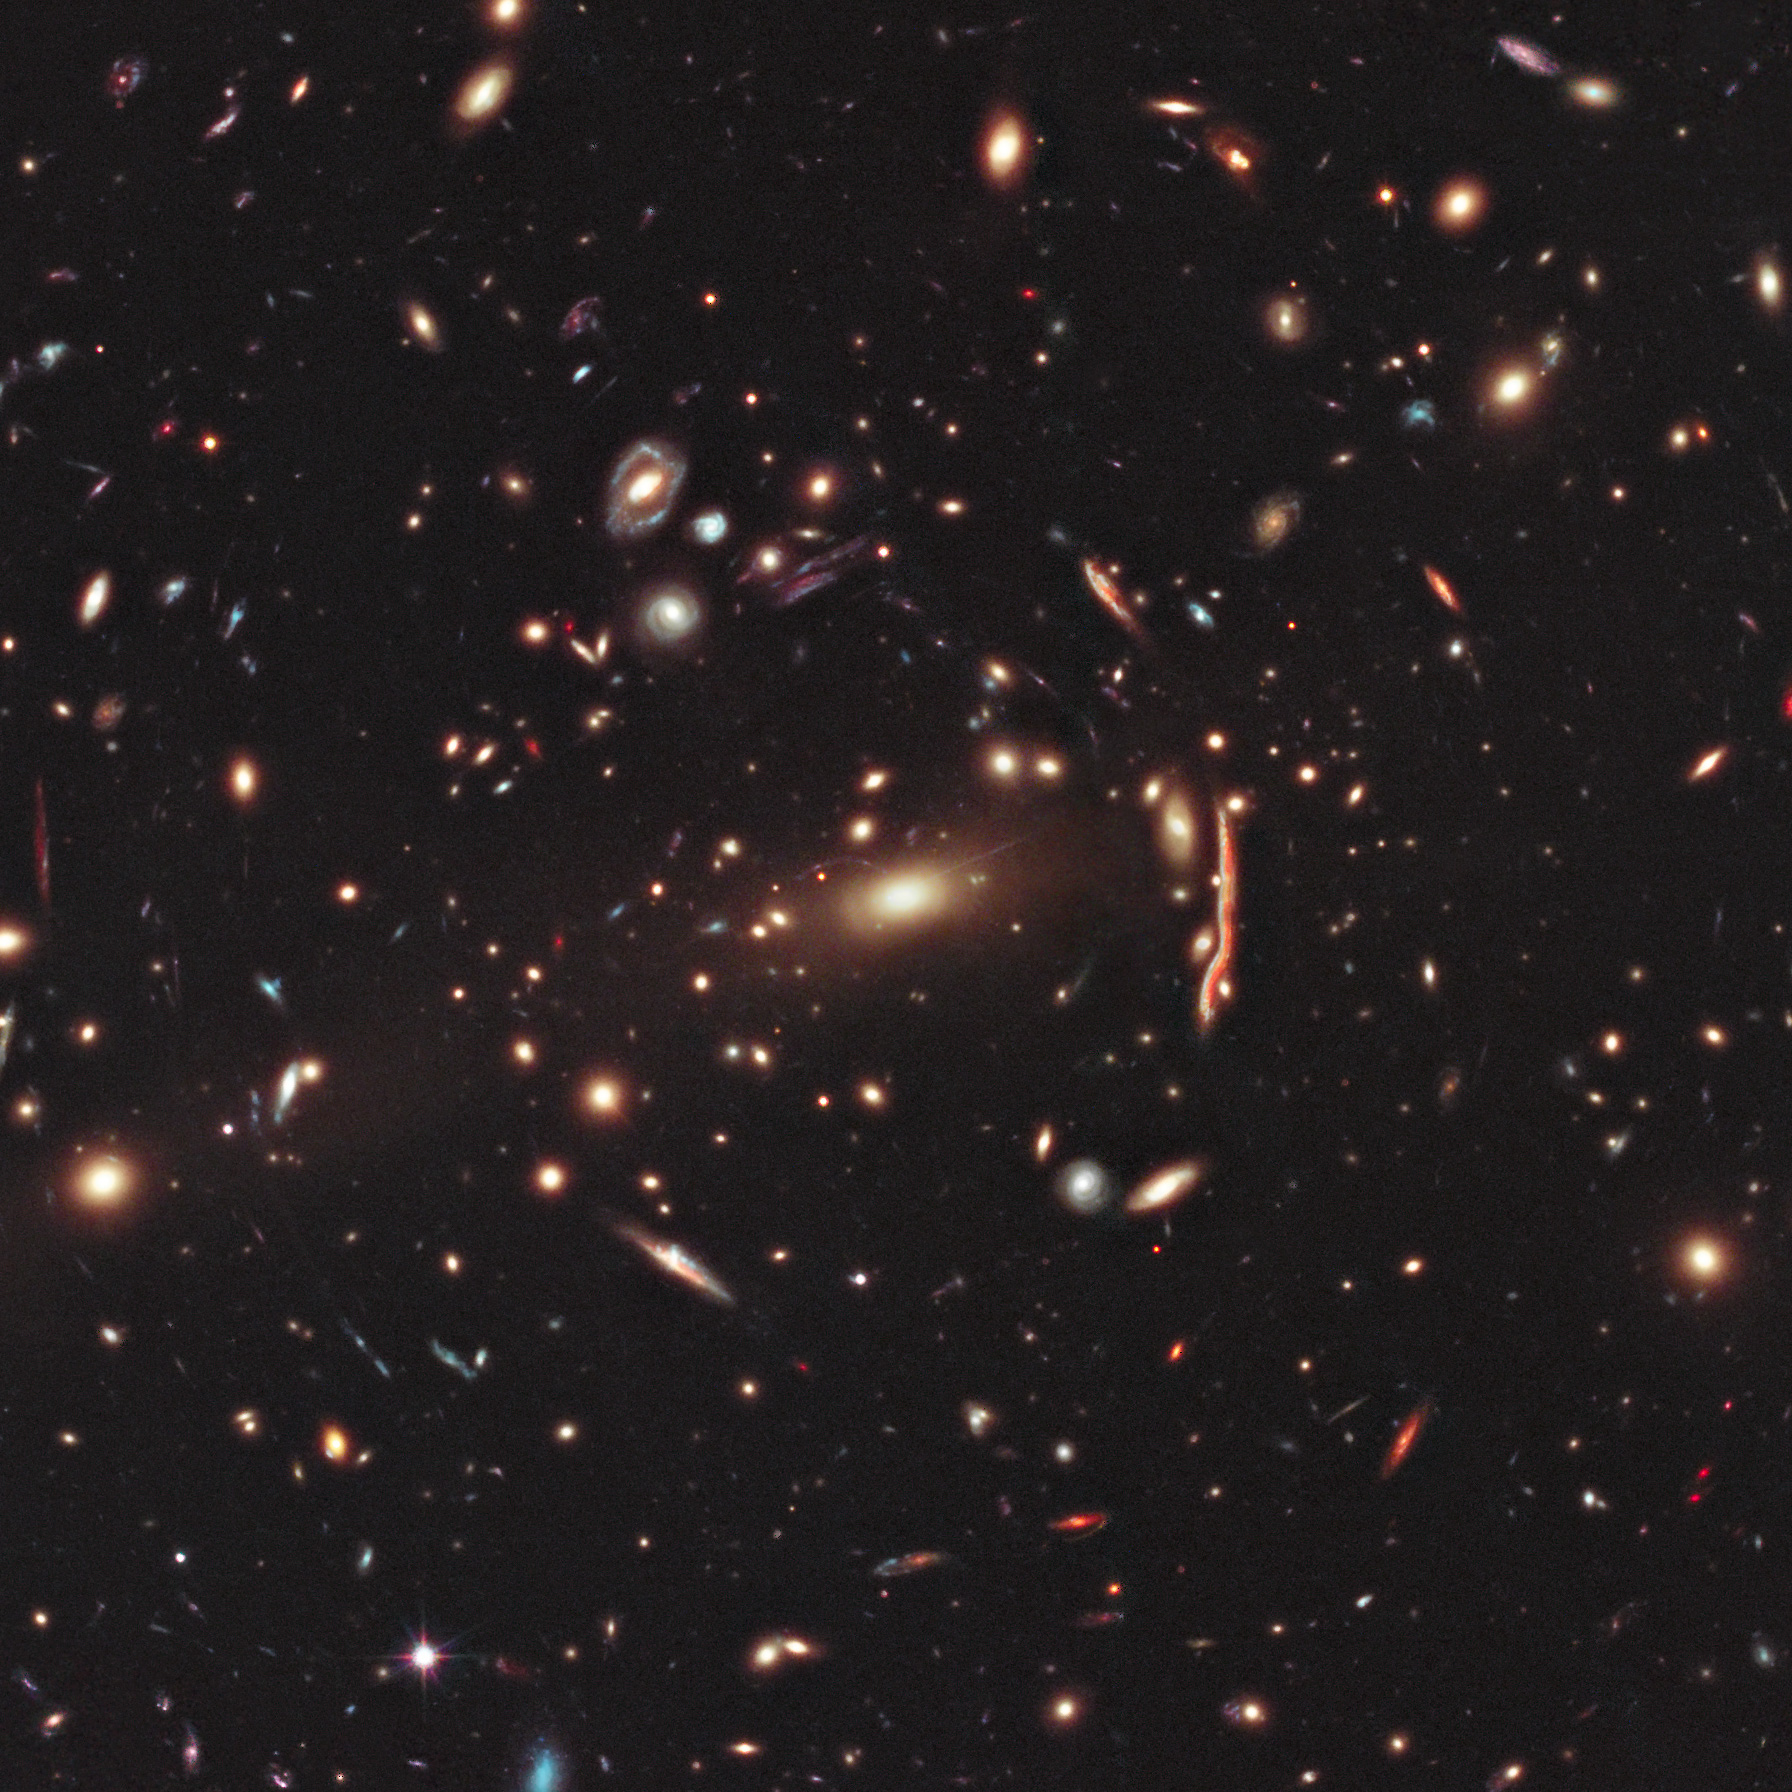
\includegraphics[width=\textwidth]{images/gravitation-lensing-macs-j1206-nasa-square-crop}
\vskip 0pt
\caption{Hubble Space Telescope image of galaxy cluster MACS J1206 showing visible distortion due to gravitational lensing. Image credit: ESA/Hubble.}
\label{sfig:gravitational-lensing-photo}
\end{subfigure}%
\hspace*{\fill}
\begin{subfigure}[b]{.46\linewidth}
\vskip 0pt
\centering
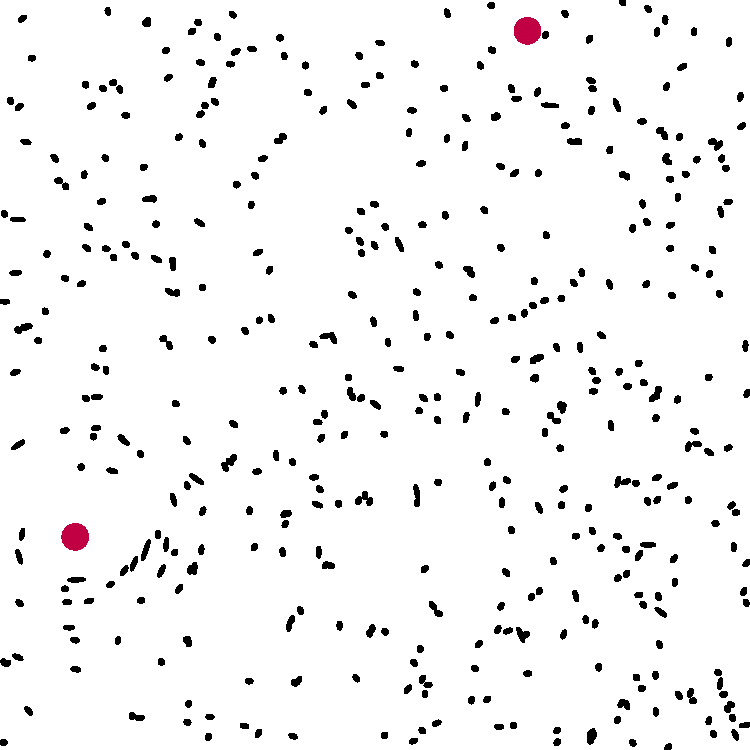
\includegraphics[width=\textwidth]{images/simulated-galaxy-cluster}
\vskip 0pt
\caption{Simulated galaxy cluster image from \emph{Observing Dark Worlds} data \citep{kaggle2012observing} showing ellipticity of galaxies (black ellipses) distorted by dark matter halos (red circles).}
\label{sfig:gravitational-lensing-simulated}
\end{subfigure}%
\caption[Examples of gravitational lensing.]{Gravitational lensing in real and simulated galaxy cluster images.}
\label{fig:gravitational-lensing}
\end{figure}

Having now introduced the tools we use to construct probabilistic models, we will now describe more concretely the task of inference. To help motivate our exposition we will discuss inference in the context of a specific problem: inferring the location of dark matter halos from the observed gravitational lensing of light emitted by surrounding galaxies. This task was the inspiration for a Kaggle\footnote{An online platform for predictive modelling competitions \url{https://www.kaggle.com}.} competition, \emph{Observing Dark Worlds} \citep{kaggle2012observing,harvey2014observing} and we will use the simplified formulation of the task used in the competition as the basis for our discussion here.% and model we present is based on the reports of two of the winning participants of that competition \citep{murray2012bayesian,salimans2012observing}.

\subsection{Example problem: Observing Dark Worlds}

We will begin with a brief review of the motivation for the \emph{Observing Dark Worlds} inference problem. Dark matter is a hypothesised form of matter which does not emit or interact with electromagnetic radiation.  This prevents direct observation of dark matter by telescopes as it produces no signal in any part of the electromagnetic spectrum \citep{massey2010dark}. General relativity however predicts that all objects with mass locally distort spacetime. If a very large concentration of mass lies between an observer and a light source the strong distortion of spacetime by the mass significantly alters the paths of photons emitted by the source and causes the apparent image of the source to the observer to be visibly distorted \citep{bartelmann2001weak}. This effect is analagous to placing a lens between the light source and observer and this motivates the term \emph{gravitational lensing} to describe the phenonemon. It is believed that large concentrations of dark matter around galaxy clusters termed \emph{dark matter halos}, cause gravitational lensing of the light emitted from background galaxies observed in telescope imagery of galaxy clusters. %Detection of instances of such distortion would therefore allow indirect observation of the presence and sky position of dark matter halos. 

\marginpar{In the context of gravitational lensing ellipticity is defined as a complex quantity $\epsilon = \frac{a-b}{a+b} \exp(2i\phi)$ where $a$ is the length of the ellipse major axis, $b$ the minor axis length and $\phi$ the orientation of the major axis. Here we will parameterise ellipticity terms of $e_1 = \mathrm{Re}(\epsilon) $ and $e_2 = \mathrm{Im}(\epsilon)$.}
Galaxies typically have approximately elliptical shapes in telescope images. It is assumed that the \emph{ellipticities} of observed galaxy images not subject to gravitational lensing are isotropically distributed \citep{bartelmann2001weak}: there is no preferred orientation of the galaxies to an observer on Earth. The presence of a large mass concentration such as a dark matter halo between background galaxies and a telescope however locally distorts the distribution of the ellipticities of the observed galaxy images. An example of this effect in a galaxy cluster image from the Hubble Space Telescope is shown in Figure \ref{sfig:gravitational-lensing-photo} with the galaxies showing a bias towards being oriented tangentially to the bright region at the centre of the image. Local biases in the spatial distribution of galaxy ellipticities can therefore be used to infer the location of dark matter halos.

The \emph{Observing Dark Worlds} inference task is formulated as follows. The observed data consists of the sky co-ordinates $\lbrace u_g, v_g \rbrace_{g=1}^G$ and ellipticity components $\lbrace e_{1,g}, e_{2,g} \rbrace_{g=1}^G$ of a set of $G$ galaxies. The task is given this data to infer the coordinates $\lbr \rvar{x}_h, \rvar{y}_h\rbr_{h=1}^H$ of the centers of a known number of dark matter halos present in the sky field of view. Galaxy coordinate and ellipticity data are provided for multiple cluster images each with a known number of halos present and the cluster image data are assumed to be \ac{iid}.

The \emph{Observing Dark Worlds} data is simulated thus the ground truth positions of the dark matter halos are known in reality which was required for the purposes of evaluation in the competition. An example visualisation of one of the simulated galaxy cluster images in the data set is shown in Figure \ref{sfig:gravitational-lensing-simulated}. The known positions of the dark matter halos in this image are shown by red circles\footnote{A \emph{training set} of cluster image data was provided to competition participants for which the associated true dark matter halo positions were given. This data was distinct from the \emph{test set} cluster data were the halo positions are unknown and which is the basis of the described inference problem and scoring for the competition, with the training data intended to aid initial model exploration and evaluation.}. As can be seen the halo in the lower left of this image produces a strong visible distortion in the ellipticities, however the second halo at the top right has a much less visible effect on the surrounding galaxies. %, emphasising the challenging nature of even this toy version of the task. 

The use of simulated data 
%and provision of exact galaxy positions and ellipticities rather than also requiring these to be also inferred from telescope images significantly 
 reduces the difficulty of the \emph{Observing Dark Worlds} inference task compared to working with real gravitational lensing data, however for the purposes of our discussion the task is still sufficiently complex to highlight the computational challenges involved in inference problems. Further the probabilistic approach described here is similar to that used (albeit with significantly more complex models) in methods and tools used in practice to analyse gravitational lensing data to infer dark matter properties \citep{marshall2003bayesian,jullo2007bayesian}.

%The provided data consististed of a set of $S=420$ simulated galaxy cluster images provided as vectors of the co-ordinates of each galaxy center $\lbr \vct{u}^{(s)}, \vct{v}^{(s)} \rbr_{s=1}^S$ and the associated two components of the ellipticity of each galaxy $\lbr \vct{e}^{(s)}_1, \vct{e}^{(s)}_2 \rbr_{s=1}^S$.

%In the Kaggle competition simulated data was used however similar methods to those that will be discussed here (albeit with signficantly more complex models) are employed in tools used to analyse real gravitational lensing images \citep{jullo2007bayesian}.

\subsection{Defining a model}

\begin{figure}[!t]
\vskip 0pt
\centering
\begin{tikzpicture}

  \node[latent] (xh) {$\rvar{x}_h$} ; %
  \factor[above left=of xh] {pr-xh} {right:$\mathcal{U}(0, x_{\textrm{max}})$} {} {xh} ; %
  \node[latent, below=of xh, yshift=5mm] (yh) {$\rvar{y}_h$} ; %
  \factor[below left=of yh] {pr-yh} {right:$\mathcal{U}(0, y_{\textrm{max}})$} {} {yh} ; %
  \node[const, right=5.4 of xh] (ug) {$u_g$} ; %
  \node[const] (vg) at (yh -| ug) {$v_g$} ; %
  \node[latent] (ahg) at ($(yh)!0.5!(vg)+(0,-1.5)$) {$\rvar{a}_{h,g}$} ; %
  \node[latent, left=0.5 of ahg] (rhg) {$\rvar{r}_{h,g}$} ; %
  \node[op, label={above:$\sqrt{(\rvar{x}_h - u_g)^2 + (\rvar{y}_h - v_g)^2}$}] 
    (xh_yh_ug_vg-rhg) at (xh -| ahg) {} ; %
  \factoredge {xh,ug,yh,vg} {xh_yh_ug_vg-rhg} {rhg} ; %
  \node[op, label={below right:$\textrm{atan2}\lpa v_g - \rvar{y}_h, u_g - \rvar{x}_h\rpa$}]
    (xh_yh_ug_vg-ahg) at (yh -| ahg) {} ; %
  \factoredge {xh,ug,yh,vg} {xh_yh_ug_vg-ahg} {ahg} ; %
  \op[below=1.1 of rhg] {rhg_mh_th-fhg} 
    {below:$\qquad\frac{\rvar{m}_{\scalebox{0.75}{$h$}}}{\max(\rvar{r}_{\scalebox{0.75}{$h,g$}}, \rvar{t}_{\scalebox{0.75}{$h$}})}$} {} {} ; %

  \node[latent, yshift=6mm] (mh) at (rhg_mh_th-fhg -| yh) {$\rvar{m}_h$} ; %
  \factor[above=of mh] {pr-mh} {above:$\mathrm{LogNorm}(\mu_m, \sigma_m)$} {} {mh} ; %
  \node[latent, yshift=-6mm] (th) at (rhg_mh_th-fhg -| yh) {$\rvar{t}_h$} ; %
  \factor[below=of th] {pr-th} {below:$\mathrm{LogNorm}(\mu_t, \sigma_t)$} {} {th} ; %
  \node[latent] (fhg) at (rhg_mh_th-fhg -| ahg) {$\rvar{f}_{h,g}$} ; %
  
  \factoredge {mh,th,rhg} {rhg_mh_th-fhg} {fhg} ; %
  %\draw[-{Latex[length=2mm]}] (rhg_mh_th-fhg) -- (fhg) ; %
  \node[latent, right=1.4 of ahg] (bhg) {$\rvar{b}_{h,g}$} ; %
  \node[latent, right=1.4 of fhg] (chg) {$\rvar{c}_{h,g}$} ; %
  \op[left=of bhg, xshift=-1mm] {ahg_fhg-bhg} 
    {$\rvar{f}_{h,g} \cos(2\rvar{a}_{h,g})$} {ahg,fhg} {bhg} ; %
  \op[left=of chg, xshift=-1mm] {ahg_fhg-chg} 
    {below:$\rvar{f}_{h,g} \sin(2\rvar{a}_{h,g})$} {ahg,fhg} {chg} ; %
  \node[latent, right=1.4 of bhg] (d1g) {$\rvar{d}_{1,g}$} ; %
  \node[latent, right=1.4 of chg] (d2g) {$\rvar{d}_{2,g}$} ; %
  \op[left=of d1g] {bhg-d1g} {$-\sum_{h=1}^H \rvar{b}_{h,g}$} {bhg} {d1g} ; %
  \op[left=of d2g] {chg-d2g} {$-\sum_{h=1}^H \rvar{c}_{h,g}$} {chg} {d2g} ; %
  \node[obs, right=1.4 of d1g] (e1g) {$\rvar{e}_{1,g}$} ; %
  \node[obs, right=1.4 of d2g] (e2g) {$\rvar{e}_{2,g}$} ; %
  \op[left=of e1g, xshift=-0mm] {e1gi_d1g-e1g} 
    {below:$\rvar{e}^\star_{1,g} + \rvar{d}_{1,g}$} {d1g} {e1g} ; %
  \op[left=of e2g, xshift=-0mm] {e2gi_d2g-e2g} 
    {$\rvar{e}^\star_{2,g} + \rvar{d}_{2,g}$} {d2g} {e2g} ; %
  \node[latent, above= of e1gi_d1g-e1g, yshift=-4mm] (e1gi) {$\rvar{e}^\star_{1,g}$} ;
  \draw[-] (e1gi) -- (e1gi_d1g-e1g) ; %
  \factor[left=of e1gi] {pr-e1gi} {above:$\nrm{0,\sigma^2}$} {} {e1gi} ; %
  \node[latent, below= of e2gi_d2g-e2g, yshift=4mm] (e2gi) {$\rvar{e}^\star_{2,g}$} ;
  \draw[-] (e2gi) -- (e2gi_d2g-e2g) ; %
  \factor[left=of e2gi] {pr-e2gi} {below:$\nrm{0,\sigma^2}$} {} {e2gi} ; %
  
  %\node[latent, below=of dhg_s-e2g] (s) {$\rvar{s}$} ; %
  %\draw[-] (s) -- (dhg_s-e2g) ; %
  %\draw[-] (s) to[bend left=42] (chg_s-e1g) ; %
  %\factor[right=of s, xshift=2mm] {pr-s} {above:$\textrm{Gamma}(\alpha,\beta)$} {} {s} ; %
  
  \node[const, right=8.5 of xh] (dummy1) {} ; %
  \node[const, above left=of xh, xshift=1.5mm, yshift=-2mm] (dummy2) {} ; %
  \node[const, right=5 of dummy2] (dummy3) {} ; %
  \node[const, below=6.6 of dummy2] (dummy4) {} ; %
  \node[const, right=5 of dummy4, yshift=0.1mm] (dummy5) {} ; %
  \plate {platehalo} 
    {(xh)(pr-xh)(yh)(pr-yh)(mh)(pr-mh)(th)(pr-th)(rhg)(ahg)(fhg)(bhg)(chg)(xh_yh_ug_vg-rhg)(dummy2)(dummy4)} 
    {$h\in\fset{1 \,...\, H}$}; %
  \plate {plategalaxy} 
    {(rhg)(ahg)(fhg)(bhg)(chg)(xh_yh_ug_vg-rhg)(ug)(vg)(e1g)(e2g)(e1gi)(pr-e1gi)(e2gi)(pr-e2gi)(dummy3)(dummy5)} 
    {$g\in\fset{1 \,...\, G}$}; %
\end{tikzpicture}
\vskip 5pt
\caption[Gravitational lensing model factor graph.]{Factor graph of proposed model for \emph{Observing Dark Worlds} gravitational lensing inference problem for a single cluster image.}
\label{fig:observing-dark-worlds-factor-graph}
\end{figure}

\marginpar{You cannot do inference without making assumptions\\---David Mackay}
Our starting point for tackling inference problems will be to define a probabilistic model specifying proposed relationships between the observed and non-observed quantities to be inferred. The model codifies the assumptions we make about the problem and any prior beliefs we have. In virtually all real inference problems the model will be a significantly simplified description of a much more complex underlying process, usually motivated by prior empirical observations that the behaviour proposed by the model is a reasonable description of reality. For now we will consider the model as a singular fixed object we will perform inference with. In reality probabilistic modelling and inference are an iterative process with model criticism a key part of the loop \citep{box1980sampling,gelman2013philosophy}. We will discuss some of the (computational) issues involved in probabilistic model evaluation and comparison at the end of this chapter.

For the \emph{Observing Dark Worlds} problem, a proposed probabilistic model is shown as a directed factor graph in Figure \ref{fig:observing-dark-worlds-factor-graph}\footnote{The factor graph in Figure \ref{fig:observing-dark-worlds-factor-graph} is based on the models used by the participants with the top-two winning entries in the Kaggle competition, Iain Murray and Tim Salimans, and described in their personal reports on their competition entries \citep{salimans2012observing,murray2012bayesian} and an article evaluating the competition outcomes \citep{harvey2014observing}.}. This model assumes a simple, physically motivated relationship between the dark matter halo positions and the observed spatial distribution of galaxy ellipticities. As well as random variables for the halo coordinates $\lbrace \rvar{x}_h,\rvar{y}_h \rbrace_{h=1}^H$ and galaxy ellipticity components $\lbrace \rvar{e}_{1,g},\rvar{e}_{2,g} \rbrace_{g=1}^G$, the model also introduces additional latent (non-observed) random variables $\lbrace \rvar{m}_{h}, \rvar{t}_h \rbrace_{h=1}^H$, which correpond respectively to the unknown total masses of each halo (multiplied by an arbitrary scaling factor) and an unknown \emph{core radius} for each halo, which specifies a radial distance within which the distortion by the halo is of constant magnitude. The halo coordinates are assumed to be marginally uniformly distributed across the image extents. The halo mass and core radius latent variables are both positive quanties and are assumed to have log normal marginal distributions.

The model proposes that at sky coordinate $(u,v)$ each halo produces a shear distortion of magnitude
\begin{equation}\label{eq:dark-matter-halo-force}
  f_h(u,v) = \frac{\rvar{m}_h}{\max(r_h,\rvar{t}_h)}
  \quad\textrm{where}\quad
  r_h = \sqrt{(\rvar{x}_h - u)^2 + (\rvar{y}_h - v)^2}
\end{equation}
and acting in a tangential direction to the radial vector from the halo centre $(\rvar{x}_h,\rvar{y}_h)$ to $(u,v)$. %, i.e. proportional to $\rvar{m}_h$ and of constant magnitude for galaxies with radial distance $\rvar{r}_{h,g}$ from the halo of less than the core radius $\rvar{t}_h$ and with a $\rvar{r}_{h,g}^{-1}$ dependence outside this threshold. 
This functional relationship is just one possibility among many. % - alternative models using a different $f_h$ could be used instead.
The post-competition review article \citep{harvey2014observing} revealed that the simulated data actually used dark matter halos with a mixture of two different radial density profiles, neither of which correspond to the distortion model assumed in \eqref{eq:dark-matter-halo-force}. This mismatch between a model and the actual process by which observations were generated will virtually always be the case in real inference problems. We can still make inferences which are consistent with our modelling assumptions, however we should as far as possible also critically review those modelling assumptions to check the validity of the inferences made.

For galaxies where the variation of the magnitude of the distorting effect of a halo across the extent of the galaxy's image is small, a reasonable approximation of the gravitational lensing effect of a single halo on the observed ellipticity $(\rvar{e}_{1,g},\rvar{e}_{2,g})$ of a galaxy image with intrinsic (prior to any gravitational lensing effect) ellipticity $(\rvar{e}_{1_g}^\star, \rvar{e}_2^\star)$ is that 
\begin{equation}\label{eq:obs-ellipticity-single-halo}
  \rvar{e}_{1,g} = \rvar{e}_{1,g}^\star - \rvar{f}_{h,g} \cos(2 \rvar{a}_{h,g}),
  \quad
  \rvar{e}_{2,g} = \rvar{e}_{2,g}^\star -  \rvar{f}_{h,g} \sin(2 \rvar{a}_{h,g}),
\end{equation}
where $\rvar{a}_{h,g} = \textrm{atan2}\lpa v_g - \rvar{y}_h, u_g - \rvar{x}_g\rpa$ is the angle the line from the centre of halo $h$ to galaxy $g$ makes to the horizontal axis and $\rvar{f}_{h,g} = f_h(u_g, v_g)$ is the magnitude of the shear distortion according to the proposed relationship in Equation \eqref{eq:dark-matter-halo-force} evaluated at the galaxy image centre \citep{bartelmann2001weak,marshall2003bayesian}. For clusters with multiple halos, a further simple linearity assumption is made, that the shear distortions due to the different halos act additively on the ellipticity components
\begin{equation}\label{eq:obs-ellipticity-multiple-halos}
  \rvar{e}_{1,g} = \rvar{e}_{1,g}^\star - \sum_{h=1}^H \rvar{f}_{h,g} \cos(2 \rvar{a}_{h,g}),
  ~
  \rvar{e}_{2,g} = \rvar{e}_{2,g}^\star -  \sum_{h=1}^H \rvar{f}_{h,g} \sin(2 \rvar{a}_{h,g}).
\end{equation}
The intrinsic ellipticities of the galaxies are assumed to have a isotropic, zero-mean normal distribution,  with standard deviation $\sigma$, with normal assumption corresponding well to empirical observations from large scale surveys \citep{bartelmann2001weak,marshall2003bayesian}. For now we will assume the standard deviation $\sigma$ of the intrinsic ellipticities, and the parameters $\mu_m,\,\sigma_m,\,\mu_t,\,\sigma_t$ of the halo mass and core radius marginal distributions have somehow been set to reasonable values, for example based on prior beliefs about the typical ranges of the variables. We will discuss possible strategies for choosing (or inferring) these parameters in more detail later.

%In particular we will assume the model proposes a probabilistic relationship between observable quantities, which for the purposes of this section we will assume are collected together in the random vector $\rvct{y}$, and unobserved quantities which we will group in to a random vector $\rvct{z}$. Note that here we will assume $\rvct{z}$ includes \emph{all} unobserved random variables in the model irrespective of whether they correspond to `meaningful' quantities we wish to infer the values of, or are `nuisance' variables which we have no interest in the value of.

%Implicitly or explicitly the model defines a joint probability $\prob{\rvar{y},\rvar{z}}$; this might be provided as a joint probability density $\pden{\rvar{y},\rvar{z}}$ which specifies $\prob{\rvar{y},\rvar{z}}$, or a \emph{simulator} or \emph{generative model} which allows to generate values for $\rvct{y}$ and $\rvct{z}$ without directly specification of a joint density.

\subsection{Making predictions}

Having now defined a model for the \emph{Observing Dark Worlds} problem, we now consider how to use this model to make predictions about the unobserved dark matter halo positions. The downstream task we are using the inference output for will generally determine what the exact inferential query we wish to evaluate is. In general however, any prediction output which takes into account all of the information we have about the unobserved variables given the assumed model and observed data will be computed as a conditional expectation.

To motivate this statement for the \emph{Observing Dark Worlds} example we will discuss some instances of outputs we might wish to compute. For notational convenience we define the following random vectors for the halo random variables
\begin{equation}
  \rvct{x} = \begin{bmatrix} \rvar{x}_1 \\ \vdots \\[-1mm] \rvar{x}_H \end{bmatrix},
  \quad
  \rvct{y} = \begin{bmatrix} \rvar{y}_1 \\ \vdots \\[-1mm] \rvar{y}_H \end{bmatrix},
  \quad
  \rvct{m} = \begin{bmatrix} \rvar{m}_1 \\ \vdots \\[-1mm] \rvar{m}_H \end{bmatrix},
  \quad
  \rvct{t} = \begin{bmatrix} \rvar{t}_1 \\ \vdots \\[-1mm] \rvar{t}_H \end{bmatrix},
\end{equation}
and similarly for the observed and intrinsic galaxy ellipticities
\begin{equation}
  \rvct{e}_1 = \begin{bmatrix} 
    \rvar{e}_{1,1} \\ \vdots \\[-1mm] \rvar{e}_{1,G}
  \end{bmatrix},
  \quad
  \rvct{e}_2 = \begin{bmatrix} 
    \rvar{e}_{2,1} \\ \vdots \\[-1mm] \rvar{e}_{2,G}
  \end{bmatrix},
  \quad
  \rvct{e}^\star_1 = \begin{bmatrix} 
    \rvar{e}^\star_{1,1} \\ \vdots \\[-1mm] \rvar{e}^\star_{1,G}
  \end{bmatrix},
  \quad
  \rvct{e}^\star_2 = \begin{bmatrix} 
    \rvar{e}^\star_{2,1} \\ \vdots \\[-1mm] \rvar{e}^\star_{2,G}
  \end{bmatrix}.
\end{equation}
An obvious output we may wish to compute is the expected (mean) values of the halo positions given the observed ellipticities. From a decision theoretic standpoint these values correspond to the position predictions which minimise the expected squared error loss from the true positions given the model and observed data. 
As conditonal expectations these are simply
\begin{equation}
  \vct{m}_{\rvct{x}} = \expc{\rvct{x} \gvn \rvct{e}_1 = \vct{e}_1,\,\rvct{e}_2 = \vct{e}_2}
  ~~\textrm{and}~~
  \vct{m}_{\rvct{y}} = \expc{\rvct{y} \gvn \rvct{e}_1 = \vct{e}_1,\,\rvct{e}_2 = \vct{e}_2}.
\end{equation}
We may also be interested in the covariances of the halo positions conditioned on the observations, these giving some idea of our remaining uncertainty in the positions and any correlations between them after conditioning on the observed ellipticities. Again these can be expressed as conditional expectations
\begin{align}
  \nonumber
  \mtx{C}_{\rvct{x},\rvct{x}} &=
  \expc{
    (\rvct{x}-\vct{m}_{\rvct{x}})(\rvct{x}-\vct{m}_{\rvct{x}})\tr
    \gvn \rvct{e}_1 = \vct{e}_1,\,\rvct{e}_2 = \vct{e}_2
  },
  \\
  \mtx{C}_{\rvct{y},\rvct{y}} &=
  \expc{
    (\rvct{y}-\vct{m}_{\rvct{y}})(\rvct{y}-\vct{m}_{\rvct{y}})\tr
    \gvn \rvct{e}_1 = \vct{e}_1,\,\rvct{e}_2 = \vct{e}_2
  },
  \\
  \nonumber
  \textrm{and}\quad
  \mtx{C}_{\rvct{x},\rvct{y}} &=
  \expc{
    (\rvct{x}-\vct{m}_{\rvct{x}})(\rvct{y}-\vct{m}_{\rvct{y}})\tr
    \gvn \rvct{e}_1 = \vct{e}_1,\,\rvct{e}_2 = \vct{e}_2
  }.
\end{align}
In the \emph{Observing Dark Worlds} competition, participants' halo position predictions were evaluated by comparing to the known true halo positions using a metric provided as part of the competition instructions. If we denote the metric $\ell(\vct{x},\vct{y};\hat{\vct{x}},\hat{\vct{y}})$ where $(\vct{x},\vct{y})$ are the true halo positions and $(\hat{\vct{x}},\hat{\vct{y}})$ the predicted positions, then the optimal predictions given the assumed model and observed data can be calculated by minimising the expected metric value conditioned on the observed data
\begin{equation}
  \bar{\ell}(\hat{\vct{x}},\hat{\vct{y}}) =
  \expc{\ell(\rvct{x},\rvct{y};\hat{\vct{x}},\hat{\vct{y}}) \gvn \rvct{e}_1 =\vct{e}_1, \rvct{e}_2=\vct{e}_2}.
\end{equation}
Due to linearity of the expectation operator, we can also calculate the derivatives of the expected metric with respect to the predictions as
\begin{equation}
\begin{split}
  \pd{\bar{\ell}(\hat{\vct{x}},\hat{\vct{y}})}{\hat{\vct{x}}} &=
  \expc{
    \pd{\ell(\rvct{x},\rvct{y};\hat{\vct{x}},\hat{\vct{y}})}{\hat{\vct{x}}}
    \mathrel{\Big|} \rvct{e}_1 =\vct{e}_1, \rvct{e}_2=\vct{e}_2}\\
  \textrm{and}\quad
  \pd{\bar{\ell}(\hat{\vct{x}},\hat{\vct{y}})}{\hat{\vct{y}}} &=
  \expc{
    \pd{\ell(\rvct{x},\rvct{y};\hat{\vct{x}},\hat{\vct{y}})}{\hat{\vct{y}}}
    \mathrel{\Big|} \rvct{e}_1 =\vct{e}_1, \rvct{e}_2=\vct{e}_2}.
\end{split}
\end{equation}
For some metrics we will be able to analytically solve for the stationary points to find the predictions minimising $\bar{\ell}(\hat{\vct{x}},\hat{\vct{y}})$ and more generally we can use the derivatives in an iterative optimisation scheme.

Evaluating conditional expectations of functions of the unobserved variables in a model given observed data is therefore the key computational task in making inferences about the variables in a probabilistic model. The \emph{Observing Dark Worlds} model factor graph in Figure \ref{fig:observing-dark-worlds-factor-graph} defines a joint density across all the variables in the model. We can therefore use Equation \eqref{eq:conditional-expectation-density} to write the conditional expectation of a measurable function $f$ of the halo position random variables $\rvct{x}$ and $\rvct{y}$ as\footnote{For brevity the sets on which integrals are evaluated have been omitted in this section and should be assumed to be the full co-domain of the corresponding random vector.}
\begin{equation}\label{eq:odw-conditional-expectation}
\begin{split}
  \expc{f(\rvct{x},\rvct{y}) \gvn \rvct{e}_1 =\vct{e}_1, \rvct{e}_2=\vct{e}_2} =&\\
  \iint
    f(\vct{x},\vct{y})\,
    &\pden{\rvct{x},\rvct{y} | \rvct{e}_1,\rvct{e}_2}(\vct{x},\vct{y} \gvn \vct{e}_1,\vct{e}_2)
  \,\dr\vct{x}\,\dr\vct{y},
\end{split}
\end{equation}
where the conditional density $\pden{\rvct{x},\rvct{y} | \rvct{e}_1,\rvct{e}_2}$ is defined as
\begin{equation}
  \pden{\rvct{x},\rvct{y} | \rvct{e}_1,\rvct{e}_2}(\vct{x},\vct{y} \gvn \vct{e}_1,\vct{e}_2) =
  \frac
    {\pden{\rvct{x},\vct{y},\rvct{e}_1,\rvct{e}_2}(\vct{x},\vct{y},\vct{e}_1,\vct{e}_2)}
    {\pden{\rvct{e}_1,\rvct{e}_2}(\vct{e}_1,\vct{e}_2)},
\end{equation}
with $\pden{\rvct{e}_1,\rvct{e}_2}$ defined in terms of $\pden{\rvct{x},\rvct{y},\rvct{e}_1,\rvct{e}_2}$ by marginalising out $\rvct{x}$ and $\rvct{y}$
\begin{equation}
  \pden{\rvct{e}_1,\rvct{e}_2}(\vct{e}_1,\vct{e}_2) =
  \iint 
    \pden{\rvct{x},\rvct{y},\rvct{e}_1,\rvct{e}_2}(\vct{x},\vct{y},\vct{e}_1,\vct{e}_2) 
  \,\dr\vct{x}\,\dr\vct{y}.
\end{equation}
We can express $\pden{\rvct{x},\vct{y},\rvct{e}_1,\rvct{e}_2}$ itself as a marginal of the joint density over all random variables in the model (which we can read off as a product of factors from Figure \ref{fig:observing-dark-worlds-factor-graph}) by marginalising out $\rvct{m}$, $\rvct{t}$, $\rvct{e}_1^\star$ and $\rvct{e}_2^\star$
\begin{equation}\label{eq:odw-e1-e2-x-y-joint-1}
\begin{split}
  \pden{\rvct{x}, \rvct{y}, \rvct{e}_1,\rvct{e}_2}(\vct{x},\vct{y},\vct{e}_1,\vct{e}_2) =
  \iiiint &
    \pden{\rvct{x}}(\vct{x}) \, 
    \pden{\rvct{y}}(\vct{y}) \, 
    \pden{\rvct{m}}(\vct{m}) \,
    \pden{\rvct{t}}(\vct{t}) \,
    \\[-1.5mm]& 
    \pden{\rvct{e}_1 | \rvct{e}_1^\star\kern-2pt,\rvct{x},\rvct{y},\rvct{m},\rvct{t}}
    (\vct{e}_1\gvn\vct{e}_1^\star\kern-2pt,\vct{x},\vct{y},\vct{m},\vct{t})\,
    \\&    
    \pden{\rvct{e}_2 | \rvct{e}_2^\star\kern-1.5pt,\rvct{x},\rvct{y},\rvct{m},\rvct{t}}
    (\vct{e}_2\gvn\vct{e}_2^\star\kern-1.5pt,\vct{x},\vct{y},\vct{m},\vct{t})\,
    \\&
    \pden{\rvct{e}_1^\star}(\vct{e}_1^\star) \, 
    \pden{\rvct{e}_2^\star}(\vct{e}_2^\star) \,
    \dr\vct{e}_1^\star\dr\vct{e}_2^\star\dr\vct{t}\,\dr\vct{m}.
\end{split}
\end{equation}
The integration with respect to $\vct{e}_1^\star$ and $\vct{e}_2^\star$ can be performed analytically as the conditional density factors $\pden{\rvct{e}_2 | \rvct{e}_2^\star\kern-2pt,\rvct{x},\rvct{y},\rvct{m},\rvct{t}}$ and $\pden{\rvct{e}_2 | \rvct{e}_1^\star\kern-2pt,\rvct{x},\rvct{y},\rvct{m},\rvct{t}}$ correspond to deterministic factors which depend linearly on $\rvct{e}_1^\star$ and $\rvct{e}_2^\star$. Expressing the deterministic factors as Dirac deltas and denoting the functions corresponding to the computational graphs in Figure \ref{fig:observing-dark-worlds-factor-graph} mapping from $\fset{\rvar{x}_h,\rvar{y}_h,\rvar{m}_h,\rvar{t}_h}_{h=1}^H$ to $\lbrace \rvar{d}_{1,g}\rbrace_{g=1}^G$ and $\lbrace \rvar{d}_{2,g} \rbrace_{g=1}^G$, $\vct{d}_1$ and $\vct{d}_2$ respectively, we have that
\begin{equation}\label{eq:odw-e1-gvn-xymt}
\begin{split}
  &\pden{\rvct{e}_1 | \rvct{x},\rvct{y},\rvct{m},\rvct{t}} (\vct{e}_1\gvn\vct{x},\vct{y},\vct{m},\vct{t})
  \\
  &\qquad=
  \int 
    \pden{\rvct{e}_1 | \rvct{e}_1^\star\kern-2pt,\rvct{x},\rvct{y},\rvct{m},\rvct{t}}
    (\vct{e}_1\gvn\vct{e}_1^\star\kern-2pt,\vct{x},\vct{y},\vct{m},\vct{t})\,
    \pden{\rvct{e}^\star_1}(\vct{e}^\star_1)
  \,\dr\vct{e}^\star_1 
  \\
  &\qquad=
  \int 
    \delta\lpa
     \vct{e}_1 - \vct{e}^\star_1 - \vct{d}_1(\vct{x},\vct{y},\vct{m},\vct{t})
    \rpa\,
    \nrm{\vct{e}^\star_1 \gvn \vct{0},\sigma^2\mathbf{I}}
  \,\dr\vct{e}^\star_1\\
  &\qquad=
  \nrm{\vct{e}_1 \gvn \vct{d}_1(\vct{x},\vct{y},\vct{m},\vct{t}),\sigma^2\mathbf{I}},
\end{split}
\end{equation}
and likewise for $\pden{\rvct{e}_2 | \rvct{x},\rvct{y},\rvct{m},\rvct{t}}$
\begin{equation}\label{eq:odw-e2-gvn-xymt}
  \pden{\rvct{e}_2 | \rvct{x},\rvct{y},\rvct{m},\rvct{t}}(\vct{e}_2\gvn\vct{x},\vct{y},\vct{m},\vct{t})
  =
  \nrm{\vct{e}_2 \gvn \vct{d}_2(\vct{x},\vct{y},\vct{m},\vct{t}),\sigma^2\mathbf{I}}.
\end{equation}
%If we define $\rvct{n} = \log \rvct{m}$ and $\rvct{u} = \log \rvct{t}$ then as $\lbrace \rvar{m}_h \rbrace_{h=1}^H$ and $\lbrace \rvar{t}_h \rbrace_{h=1}^H$ have log-normal marginal densities, then $\rvct{n}$ and $\rvct{u}$ will have multivariate normal densities, $\pden{\rvct{n}}(\vct{n}) = \nrm{\vct{n} \gvn \mu_m\vct{1}, \sigma_m^2\mathbf{I}}$ and $\pden{\rvct{u}}(\vct{u}) = \nrm{\vct{u} \gvn \mu_t\vct{1}, \sigma_t^2\mathbf{I}}$.
%\begin{equation}
%\begin{split}
%  &\pden{\rvct{x},\rvct{y},\rvct{e}_1,\rvct{e}_2}(\vct{x},\vct{y},\vct{e}_1,\vct{e}_2) = \\
%  &\qquad
%  \frac{1}{x_{\textrm{max}}^H \, y_{\textrm{max}}^H}
%  \prod_{h=1}^H \lpa 
%    \ind{[0,x_{\textrm{max}}]}(x_h) \,
%    \ind{[0,y_{\textrm{max}}]}(y_h) 
%  \rpa 
%  \\
%  &\qquad
%  \iint
%    \nrm{\vct{n} \gvn \mu_m\vct{1}, \sigma_m^2\mathbf{I}} \, 
%    \nrm{\vct{u} \gvn \mu_m\vct{1}, \sigma_m^2\mathbf{I}}
%  \\[-1.5mm]
%  &\qquad\phantom{\iint}\,
%    \nrm{\vct{e}_1 \gvn -\vct{d}_1(\vct{x},\vct{y},\exp\vct{n},\exp\vct{u}),\sigma^2\mathbf{I}}\,
%  \\
%  &\qquad\phantom{\iint}\,
%    \nrm{\vct{e}_2 \gvn -\vct{d}_2(\vct{x},\vct{y},\exp\vct{n},\exp\vct{u}),\sigma^2\mathbf{I}}
%  \,\dr\vct{u}\,\dr\vct{n}
%\end{split}
%\end{equation}
Rewriting \eqref{eq:odw-e1-e2-x-y-joint-1} in terms of \eqref{eq:odw-e1-gvn-xymt} and \eqref{eq:odw-e2-gvn-xymt} and substituting the definitions for the factors from Figure \ref{fig:observing-dark-worlds-factor-graph} we have that
\begin{equation}\label{eq:odw-e1-e2-x-y-joint-2}
\begin{split}
  &\pden{\rvct{x},\rvct{y},\rvct{e}_1,\rvct{e}_2}(\vct{x},\vct{y},\vct{e}_1,\vct{e}_2) =
  \iint 
    \pden
      {\rvct{x},\rvct{y},\rvct{m},\rvct{t},\rvct{e}_1,\rvct{e}_2}
      (\vct{x},\vct{y},\vct{m},\vct{t},\vct{e}_1,\vct{e}_2)
   \,\dr\vct{t}\,\dr\vct{m}
  \\
  &
  ~=\iint
  \prod_{h=1}^H \lpa 
    \mathcal{U}\lpa x_h \gvn 0,x_{\textrm{max}}\rpa \,
    \mathcal{U}\lpa y_h \gvn 0,y_{\textrm{max}}\rpa 
  \rpa 
  \\
  &
  \phantom{~=\iint}~
    \nrm{\vct{e}_1 \gvn \vct{d}_1(\vct{x},\vct{y},\vct{m},\vct{t}),\sigma^2\mathbf{I}}\,
    \nrm{\vct{e}_2 \gvn \vct{d}_2(\vct{x},\vct{y},\vct{m},\vct{t}),\sigma^2\mathbf{I}}
  \\
  &\phantom{~=\iint}~
    \textrm{LogNorm}\lpa \vct{m} \gvn \mu_m\vct{1}, \sigma_m^2\mathbf{I} \rpa \, 
    \textrm{LogNorm}\lpa \vct{t} \gvn \mu_m\vct{1}, \sigma_m^2\mathbf{I} \rpa
  \,\dr\vct{t}\,\dr\vct{m}.
\end{split}
\end{equation}
We cannot simplify this integral any further analytically. Thefore the conditional expectation we wish to compute in terms of integrals of functions we can evaluate pointwise is
\begin{equation}\label{eq:odw-cond-expectation-2}
\begin{split}
  &\expc{f(\rvct{x},\rvct{y}) \gvn \rvct{e}_1 =\vct{e}_1, \rvct{e}_2=\vct{e}_2} = \\
  &
  \frac
  {\displaystyle
    \iiiint f(\vct{x},\vct{y}) \, 
    \pden
      {\rvct{x},\rvct{y},\rvct{m},\rvct{t},\rvct{e}_1,\rvct{e}_2}
      (\vct{x},\vct{y},\vct{m},\vct{t},\vct{e}_1,\vct{e}_2)
    \,\dr\vct{t}\,\dr\vct{m}\,\dr{\vct{x}}\,\dr{\vct{y}}
  }
  {\displaystyle
    \iiiint
      \pden
      {\rvct{x},\rvct{y},\rvct{m},\rvct{t},\rvct{e}_1,\rvct{e}_2}
      (\vct{x},\vct{y},\vct{m},\vct{t},\vct{e}_1,\vct{e}_2)
    \,\dr\vct{t}\,\dr\vct{m}\,\dr{\vct{x}}\,\dr{\vct{y}}
  }.
\end{split}
\end{equation}
Each of the vector integration variables in \eqref{eq:odw-cond-expectation-2} is of dimension $H$ and so the overall dimension of the space being integrated over in both the numerator and denominator is $4H$.
In the \emph{Observing Dark Worlds} data the number of halos per cluster image $H$ is between one and three so to evaluate conditional expectations of the halo positions we need to compute integrals over spaces with four, eight or twelve dimensions. 

For four or eight dimensions it may be feasible to use quadrature methods \citep{davis1967numerical}, which involve evaluating the integrand across a fixed grid of points and then computing a weighted sum of these values, to numerically approximate the integrals to reasonable accuracy. For a fixed grid resolution however the cost of quadrature scales exponentially with the dimension of the space being integrated over - if $N$ points are used per dimension, using quadrature to evaluate \eqref{eq:odw-cond-expectation-2} will involve $N^{4H}$ evaluations of the integrand. 

Assuming the computational cost of the function $f(\rvct{x},\rvct{y})$ the conditional expectation is being calculated of is negligible, the dominant cost in the evaluation of the integrands in \eqref{eq:odw-cond-expectation-2} will be in evaluating $\vct{d}_1(\vct{x},\vct{y},\vct{m},\vct{t})$ and $\vct{d}_2(\vct{x},\vct{y},\vct{m},\vct{t})$ which involve computing the distances and angles between all galaxy-halo pairs. Using a very simplistic (and conservative) assumption that each arithmetic, square root, comparison and trigonometric operation has a unit floating point operation cost, the computation graph in Figure \ref{fig:observing-dark-worlds-factor-graph} which is present on the overlap between the two plates will involve 15 floating point operations in a single forward pass and is evaluated $GH$ times for an overall cost per integrand evaluation of $15GH$ floating point operations. 

A rough but conservative lower bound on the floating point operation count of evaluating the integrals in \eqref{eq:odw-cond-expectation-2} using quadrature is therefore $15 GH N^{4H}$. The number of galaxies $G$ per cluster image in the \emph{Observing Dark Worlds} data varies between 300 and 740. If we assume $G=500$ and that we use $N=20$ grid points per dimension, for the $H=2$ cases evaluating the conditional expectation will involve $\sim 1\times 10^9$ floating point operations, for $H=2$, $\sim 4 \times 10^{14}$ floating point operations and for $H=3$, $\sim 9\times 10^{19}$ floating point operations.

At the time of writing, the theoretical peak floating point operation performance of a top-end multi-core server \ac{CPU} is around $5 \times 10^{11}$ \ac{FLOPS}. Assuming this peak performance could be obtained when using quadrature to approximate \eqref{eq:odw-cond-expectation-2}
% (an optimistic but not completely terrible assumption as the computation is trivially paralleisable across the cores)
, our back-of-the-envelope calculation suggests a trivial two millisecond compute time for clusters with one halo, a more noticeable thirteen minute computation for clusters with two halos, and an impractical six year wait for clusters with three halos.

Current top-end \acp{GPU} have a peak theoretical (single-precision) floating point performance of around $10^{13}$ \ac{FLOPS} which at best would cut the computation time for a $H=3$ case by a factor of 20 to around 100 days. With a cluster of \ac{CPU} or \ac{GPU} nodes, or faster individual nodes due to future growth in processing power, the compute time could potentially be brought down further to more reasonable timescales. However the key point in this example is the exponential growth with dimension - even moving from eight to twelve dimensions made compute time impractical. Clearly therefore approximating the integrals in expectations like \eqref{eq:odw-cond-expectation-2} using quadrature methods is not viable when performing inference in models with large numbers of unobserved variables, with the example here showing that even integrals over what might initially seem a low dimensionality of twelve can be problematic.

\subsection{Implicit models}\label{subsec:implicit-models}

In the \emph{Observing Dark Worlds} example it was possible to analytically integrate out the random vectors $\rvct{e}_1^\star$ and $\rvct{e}_2^\star$, which correspond to the intrinsic galaxy ellipticities, due to the observed ellipticities $\rvct{e}_1$ and $\rvct{e}_2$ being deterministic linear functions of $\rvct{e}_1^\star$ and $\rvct{e}_2^\star$ respectively (for fixed $\rvct{x}$, $\rvct{y}$, $\rvct{m}$ and $\rvct{t}$). Rather than calculating the conditional densities on $\rvct{e}_1$ and $\rvct{e}_2$ by integrating out $\rvct{e}_1^\star$ and $\rvct{e}_2^\star$, we could equivalently have applied the change of variables formula \eqref{eq:change-of-variables-vector-bijective} for a bijective transformation; in this case the Jacobian determinant is simply one.

\begin{figure}[t]
\centering
\begin{subfigure}[b]{.48\linewidth}
\centering
\begin{tikzpicture}
  \node[obs] (x) {$\rvar{x}$} ; %
  \node[latent, above left=0.75 and 1.5 of x] (u) {$\rvar{u}$} ; %
  \node[latent, below left=0.75 and 1.5 of x] (v) {$\rvar{v}$} ; %
  \factor[left=of u] {pr-u} {below:$\nrm{0,1}$} {} {u} ; %
  \factor[left=of v] {pr-v} {$\nrm{0,1}$} {} {v} ; %
  \op[left=of x] {u_v-x} {left:$\displaystyle\frac{\rvar{u}\rvar{v}}{\lpa 1+\exp\rvar{u}\rpa\lpa1+\exp\rvar{v}\rpa}$} {u,v} {x} ; %
\end{tikzpicture}
\caption{Directed factor graph defining model with two latent variables $(\rvar{u}, \rvar{v})$, and an observed variable $\rvar{x}$.}
\label{sfig:simple-impl-factor-graph}
\end{subfigure}
~~
\begin{subfigure}[b]{.48\linewidth}
\centering
\pgfplotsset{cycle list/Dark2-3}
\begin{tikzpicture}
  \begin{axis}[
    cycle list name={Dark2-3},
    domain=-5:5,
    xmin=-5, xmax=5,
    ymin=-5, ymax=5,
    width=48mm,
    height=48mm,
    xlabel={\small $u$},
    ylabel={\small $v$},
    every tick label/.append style={font=\tiny},
    axis y line=center,
    axis x line=middle,
    ytick={-5,5},
    xtick={-5,5},
    legend image post style={scale=0.5},
    legend style={
      at={(0.55,0.2)},
      fill=none,
      anchor=north west,
      draw=none, 
      font=\scriptsize,
    }
  ]
    \draw[gray] (axis cs:0,0) circle [radius=2.15];
    \draw[gray] (axis cs:0,0) circle [radius=1.55];
    \draw[gray] (axis cs:0,0) circle [radius=1.18];
    \draw[gray] (axis cs:0,0) circle [radius=0.84];
    \draw[gray] (axis cs:0,0) circle [radius=0.46];
    \addlegendimage{no markers,gray}
    \addlegendentry{$\pden{\rvar{u},\rvar{v}}$};
    \addplot+[mark=none, thick] table [x=u, y=v, col sep=comma] 
      {data/example-implicit-model-curve-1.csv};
    \addlegendentry{$\rvar{x} = 1$};
    
\end{axis}
\end{tikzpicture}
\caption{Plot of density on latent variables (contours) and set of values for which $\rvar{x} = 1$ (green curve).}
\label{sfig:example-implicit-model-cond-plot}
\end{subfigure}
\caption[Example of implicit probabilistic model.]{Simple example of an implicit probabilistic model where the observed variable is a non-bijective function of two latent variables.}
\label{fig:example-non-bijective-transform-factor-graph}
\end{figure}

If the observed variables had instead been the output of a deterministic factor where there was no bijective dependence on any of the parent variables (inputs to the deterministic factor), the simplified form of the change of variables formula \eqref{eq:change-of-variables-vector-bijective} would no longer have applied and instead the more general form \eqref{eq:change-of-variables-vector} would have been required. Generally in such cases it will not be possible to analytically marginalise out a parent variable to give an explicit conditional density on the observed variable(s). Models which do not admit explicit conditional densities on the observed variables are sometimes described as \emph{implicit models} \citep{diggle1984monte}, with simulator models being a common case.

An illustration of such a case for a simple three variable model is shown in Figure \ref{fig:example-non-bijective-transform-factor-graph}. Here the observed variable $\rvar{x}$ is a deterministic function of two latent (unobserved) variables $\rvar{u}$ and $\rvar{v}$. There is no analytic solution in terms of elementary functions for $\rvar{u}$ as a function of $\rvar{x}$ and $\rvar{v}$ or for $\rvar{v}$ as a function of $\rvar{x}$ and $\rvar{u}$. This means the Dirac delta term corresponding to the deterministic factor cannot be integrated out. Due to the presence of the Dirac delta the joint density $\pden{\rvar{x},\rvar{u},\rvar{v}}$ is not well defined (the joint probability $\prob{\rvar{x},\rvar{u},\rvar{m}}$ is not absolutely continuous with respect to any measure) which complicates evaluations of conditional expectations such as $\expc{f(\rvar{u},\rvar{v}) \gvn \rvar{x} = 1}$. 

In particular the set of $\rvar{u}$ and $\rvar{v}$ values corresponding to solutions to $\rvar{x} = 1$ (illustrated as the green curve in Figure \ref{sfig:example-directed-graphical-model}) has zero Lebesgue measure. Therefore even though the dimensionality is low in this case we can not use simple quadrature to evaluate conditional expectations without some further form of approximation. We will revisit methods for performing inference in implicit models later in the thesis.

\subsection{Conjugacy and exact inference}\label{subsec:conjugacy-and-exact-inference}

\begin{table}[!t]
\centering
\begin{tabular}{rl}
  \toprule
  \multicolumn{1}{c}{\textsf{Original factorisation}} & \multicolumn{1}{c}{\textsf{Conjugate factorisation}} \tabularnewline
  \midrule
  \tikz{
    \node[latent] (x) {$\rvar{x}$} ; %
    \node[latent, left=of x] (z) {$\rvar{z}$} ; %
    \factor[left=of z, xshift=-2mm] {pr-z} {$\nrm{\mu,\sigma^2}$} {} {z} ; %
    \factor[left=of x] {z-x} {$\nrm{\rvar{z},s^2}$} {z} {x}; %
    \node[const, right=0.3 of x] (dummy) {} ; %
    \draw[-, densely dotted] (x) -- (dummy) ; %
  } &
  \tikz{
    \node[latent] (x) {$\rvar{x}$} ; %
    \node[latent, left=3 of x] (z) {$\rvar{z}$} ; %
    \factor[above=of x] {pr-x} {right:$\nrm{\mu,\sigma^2+s^2}$} {} {x} ; %
    \factor[left=of x, xshift=-9mm] {x-z} {$\nrm{\frac{\sigma^2\rvar{x} + s^2\mu}{\sigma^2 + s^2}, \frac{\sigma^2 s^2}{\sigma^2 + s^2}}$} {x} {z}; %
    \node[const, right=0.3 of x] (dummy) {} ; %
    \draw[-, densely dotted] (x) -- (dummy) ; %
  } \\
  \tikz{
    \node[latent] (x) {$\rvct{x}$} ; %
    \node[latent, left=of x] (z) {$\rvct{z}$} ; %
    \factor[left=of z, xshift=-2mm] {pr-z} {$\nrm{\vct{\mu},\mtx{\Sigma}}$} {} {z} ; %
    \factor[left=of x] {z-x} {$\nrm{\rvct{z},\mtx{C}}$} {z} {x}; %
    \node[const, right=0.3 of x] (dummy) {} ; %
    \draw[-, densely dotted] (x) -- (dummy) ; %
  } &
  \tikz{
    \node[latent] (x) {$\rvct{x}$} ; %
    \node[latent, left=3 of x] (z) {$\rvct{z}$} ; %
    \factor[above=of x] {pr-x} {right:$\nrm{\vct{\mu},\mtx{\Sigma}+\mtx{C}}$} {} {x} ; %
    \factor[left=of x, xshift=-9mm] {x-z} {} {x} {z}; %
    \node[align=left, anchor=south] (lab1) at (x-z.north) {\tiny$\nrm{\mtx{D}(\mtx{C}^{-1}\rvct{x} + \mtx{\Sigma}^{-1}\vct{\mu}), \mtx{D}}$} ; %
    \node[align=left, anchor=north] (lab2) at (x-z.south) {\tiny$\textrm{where}~ \mtx{D} = (\mtx{C}^{-1}+\mtx{\Sigma}^{-1})^{-1}$} ; %
    \node[const, right=0.3 of x] (dummy) {} ; %
    \draw[-, densely dotted] (x) -- (dummy) ; %
  } \\
  \tikz{
    \node[latent] (x) {$\rvar{x}$} ; %
    \node[latent, left=of x] (z) {$\rvar{z}$} ; %
    \factor[left=of z, xshift=-2mm] {pr-z} {$\textrm{Gamma}\lpa\alpha,\beta\rpa$} {} {z} ; %
    \factor[left=of x] {z-x} {$\nrm{\mu,\frac{1}{\rvar{z}}}$} {z} {x}; %
    \node[const, right=0.3 of x] (dummy) {} ; %
    \draw[-, densely dotted] (x) -- (dummy) ; %
  } &
  \tikz{
    \node[latent] (x) {$\rvar{x}$} ; %
    \node[latent, left=3 of x] (z) {$\rvar{z}$} ; %
    \factor[above=of x] {pr-x} {right:$\textrm{StT}\lpa 2\alpha,\mu,\sqrt{\frac{\beta}{\alpha}}\rpa$} {} {x} ; %
    \factor[left=of x, xshift=-9mm] {x-z} {$\textrm{Gamma}\lpa\alpha + \frac{1}{2}, \beta + \frac{1}{2}(\rvar{x}-\mu)^2\rpa$} {x} {z}; %
    \node[const, right=0.3 of x] (dummy) {} ; %
    \draw[-, densely dotted] (x) -- (dummy) ; %
  } \\
  \tikz{
    \node[latent] (x) {$\rvar{x}$} ; %
    \node[latent, left=of x] (z) {$\rvar{z}$} ; %
    \factor[left=of z, xshift=-2mm] {pr-z} {$\textrm{Gamma}\lpa\alpha,\beta\rpa$} {} {z} ; %
    \factor[left=of x] {z-x} {$\textrm{Exp}(\rvar{z})$} {z} {x}; %
    \node[const, right=0.3 of x] (dummy) {} ; %
    \draw[-, densely dotted] (x) -- (dummy) ; %
  } &
  \tikz{
    \node[latent] (x) {$\rvar{x}$} ; %
    \node[latent, left=3 of x] (z) {$\rvar{z}$} ; %
    \factor[above=of x] {pr-x} {right:$\textrm{Lomax}\lpa \alpha, \beta\rpa$} {} {x} ; %
    \factor[left=of x, xshift=-9mm] {x-z} {$\textrm{Gamma}\lpa\alpha + \frac{1}{2}, \beta + \rvar{x}\rpa$} {x} {z}; %
    \node[const, right=0.3 of x] (dummy) {} ; %
    \draw[-, densely dotted] (x) -- (dummy) ; %
  } \\
  \tikz{
    \node[latent] (x) {$\rvar{x}$} ; %
    \node[latent, left=of x] (z) {$\rvar{z}$} ; %
    \factor[left=of z, xshift=-2mm] {pr-z} {$\textrm{Beta}(\alpha, \beta)$} {} {z} ; %
    \factor[left=of x] {z-x} {$\textrm{Ber}(\rvar{z})$} {z} {x}; %
    \node[const, right=0.3 of x] (dummy) {} ; %
    \draw[-, densely dotted] (x) -- (dummy) ; %
  } &
  \tikz{
    \node[latent] (x) {$\rvar{x}$} ; %
    \node[latent, left=3 of x] (z) {$\rvar{z}$} ; %
    \factor[above=of x] {pr-x} {right:$\textrm{Ber}\lpa \frac{\alpha}{\alpha + \beta} \rpa$} {} {x} ; %
    \factor[left=of x, xshift=-9mm] {x-z} {$\textrm{Beta}\lpa\alpha + \rvar{x}, \beta + 1 -\rvar{x}\rpa$} {x} {z}; %
    \node[const, right=0.3 of x] (dummy) {} ; %
    \draw[-, densely dotted] (x) -- (dummy) ; %
  } \\
  \bottomrule
\end{tabular}
\caption[Conjugate distribution factor graphs.]{Factor graph illustrations of conjugate distributions.}
\label{tab:conjugate-distributions}
\end{table}

Some densities have a \emph{conjugacy} property that can simplify inference. If $\rvar{x}$ and $\rvar{z}$ are two random variables in a model then the joint density on the two variable can be factorised as
\begin{equation}\label{eq:conjugate-factorisation}
  \pden{\rvar{x},\rvar{z}}(x,z) =
  \pden{\rvar{x}|\rvar{z}}(x\gvn z)\pden{\rvar{z}}(z) =
  \pden{\rvar{z}|\rvar{x}}(z\gvn x)\pden{\rvar{x}}(x).
\end{equation}
\marginpar{A conditional density $\pden{\rvct{u}|\rvct{v}}$ is from the exponential family if it can be written as\\
$\pden{\rvct{u}|\rvct{v}}(\vct{u}\gvn\vct{v})=$
\\[1mm]
$\frac{h(\vct{u}) \exp \lpa \vct{\eta}(\vct{v})\tr\vct{t}(\vct{u})\rpa}{z(\vct{v})}$,
\\[1mm] with $\vct{\eta}(\vct{v})$ termed the \emph{natural parameters} and $\vct{t}(\vct{u})$ termed the \emph{sufficient statistics}.}
For certain pairs of $\pden{\rvar{x}|\rvar{z}}$ and $\pden{\rvar{z}}$ the corresponding $\pden{\rvar{z}|\rvar{x}}$ and $\pden{\rvar{x}}$ have closed-form expressions. Some examples are shown in Table \ref{tab:conjugate-distributions}. In all of these examples $\pden{\rvar{x}|\rvar{z}}$ is a density for an \emph{exponential family distribution}. For every exponential family distribution density $\pden{\rvar{x}|\rvar{z}}$ there exists a $\pden{\rvar{z}}$ such that $\pden{\rvar{z}|\rvar{x}}$ is of the same parametric family as $\pden{\rvar{z}}$.

If $\rvar{x}$ corresponds to an observed variable in the model, then if evaluating conditional expectations $\expc{f(\rvar{z}) \gvn \rvar{x}}$ the conjugacy property means that conditional density $\pden{\rvar{z}|\rvar{x}}$ which $f$ should be integrated against has a closed form expression. Often for simple $f$, e.g. $f(z) = z$ or $f(z) = z^2$, the conditional expectations will have closed form solutions in such cases (i.e. corresponding to moments of the distribution defined by $\pden{\rvar{z}|\rvar{x}}$). Even when $f$ is more complex, typically generating independent random samples from $\pden{\rvar{z}|\rvar{x}}$ in such cases will be possible, simplifying the use of Monte Carlo methods (which will be introduced in the next chapter). If both $\rvar{z}$ and $\rvar{x}$ are latent variables then the conjugacy property is also useful as in this case $\rvar{z}$ can be analytically marginalised out of conditional expectations of functions which do not depend on $\rvar{z}$.

\begin{figure}
\centering
\begin{tikzpicture}
  \node[latent] (z0) {$\rvct{z}_{0}$} ; %
  \factor[left=of z0, xshift=-5mm] {pr-z0} {above:$\nrm{\vct{m}_0,\mtx{C}_0}$} {} {z0} ; %
  \def\T{3}
  \foreach \t in {1,...,\T} {
    \pgfmathtruncatemacro{\s}{\t-1}
    \node[latent, right=1.9 of z\s] (z\t) {$\rvct{z}_{\t}$} ; %
    \factor[left=of z\t, xshift=-5mm] {z\s-z\t} 
      {above:$\nrm{\mtx{A}_{\t}\rvct{z}_{\s} + \vct{m}_{\t}, \mtx{C}_{\t}}$} {z\s} {z\t} ; %
    \node[obs, below=of z\s, yshift=2mm] (x\s) {$\rvct{x}_{\s}$} ; %
    \factor[above=of x\s] {z\s-x\s} 
      {left:$\nrm{\mtx{B}_{\s}\rvct{z}_{\s} + \vct{n}_{\s},\mtx{D}_{\s}}$} {z\s} {x\s} ; %
  }
  \node[obs, below=of z\T, yshift=2mm] (x\T) {$\rvct{x}_{\T}$} ; %
  \factor[above=of x\T] {z\T-x\T} 
      {left:$\nrm{\mtx{B}_{\T}\rvct{z}_{\T} + \vct{n}_{\T},\mtx{D}_{\T}}$} {z\T} {x\T} ; %
\end{tikzpicture}
%\vskip 5pt
\caption[Linear dynamical system factor graph.]{Factor graph for a latent linear dynamical system model.} %
\label{fig:lds-factor-graph}
\vspace{-2mm}
\end{figure}

\marginpar{A Markov process is a stochastic process such that future states are conditionally independent of past states given the current state.}
Various algorithms have been developed to exploit conjugacy in restricted classes of probabilistic models to perform efficient exact inference. Inference in \emph{latent linear dynamical systems}, an example of which is shown as a factor graph in Figure \ref{fig:lds-factor-graph}, can be efficiently performed with the recursive Kalman filtering and smoothing algorithms \citep{kalman1960new}. Closely related are the forward and backward updates for inference in \emph{hidden Markov models} \citep{stratonovich1960conditional} which have the same factorisation structure as latent linear dynamical systems but use a discrete rather than real-valued latent state. The \emph{junction tree algorithm} \citep{lauritzen1988local} is a general purpose algorithm for performing exact inference in undirected graphical models of discrete random variables which exploits conditional independency structure to efficiently decompose the inference into local computations; the computational cost of the algorithm scales exponentially with the number of nodes in the largest clique in the model and so is mainly relevant for graphs with relatively small maximal cliques.
% message passing (link to reverse-mode AD?)

% discrete latent variables
% Boltzmann machine distribution - summation of exponential number of states
% junction tree

%In general we might consider inference as only an intermediate step with the inferential output (which we discuss in more detail below but for now we loosely define as a representation of the probable values of the unobserved random variables in our assumed model given observations) then being used in some downstream task. Achieving `optimal' in some sense performance in this task would then be considered the overall aim - decision theory offers a framework for making optimal decisions under uncertainty. Alternatively we might be interested in analysing the statistical properties of the model when conditioning on observations - for instance computing moments of variables or the probability that variables take values in within some set. Importantly in both cases however the fundamental computation involved is the same - evaluating conditional expectations of functions of the unobserved variables in the model given observations. We will generally remain agnostic to such considerations of how the output of the inference is to be used, and instead consider inference as the task of

%In general we should consider the task of inference in the context of the downstream task the inferential output is being used for. %The topic of \emph{decision theory} considers the issues surrounding using a probabilistic model to reason and make decisions under uncertainty and is a signficant research area in its own right, we will however use a very coarse but still we believe useful characterisation that the fundamental computational task in probabilistic decision theory is computing the expected value of functions of unobserved variables given a probabilistic model and observations. In particular we will assume we have a loss function we wish to minimise the expected value of (or equivalently a utitlity function we wish to maximise the expected value of).



%Given a probabilistic model and set of observations, we loosely define inference as the process of finding plausible values for the unobserved variables given the model and observations. 

%Before considering inference specifically in the setting of the \emph{Observing Dark Worlds} problem, we will first try to express the computational task in more general terms. For the sake of notational brevity we assume that we collect all observed random variables in to the random vector $\rvct{y} \in \set{Y}$ and all unobserved random variables in the model of interst in to the random vector $\rvct{z} \in \set{Z}$. Our model defines a joint probability $\prob{\rvct{y},\rvct{z}}$; in the \emph{Observing Dark Worlds} case we specified this as a directed factor graph, alternatively we might specify our model as a simulator in code or as an undirected factor graph, in all cases explicitly or implicitly we define $\prob{\rvct{y},\rvct{z}}$.

%We then define inference as the task of computing a representation of the information we have about the probable values of $\rvct{z}$ given the assumed model and observed values for $\rvct{y}$ which allows evaluation of conditional expectations $\expc{f(\rvct{z}) \gvn \rvct{y} = \vct{y}}$ of functions of the unobserved random variables. This a not entirely standard definition and not is mathematically precise, however we believe it is broadly consistent with existing usages of \emph{inference} while making clear the key property that the motivation for inference algorithm is to allow computation of (conditional) expectations.

 %Making inferences about the unobserved variables given the model and observations then fundamentally corresponds to computing conditional expectations on the unobserved variables given the observations, $\expc{f(\rvct{z}) \gvn \rvct{y} = \vct{y}}$. Conditional expectation can be used to express any inferential query we ha[align=left, anchor=north] (lab2) at (x-z.south)ve about the unobserved variables
 
\subsection{A note on Bayesian terminology}

%We have so far discussed inference without using some of the language and terminology common to discussions of \emph{Bayesian inference}. This omission was purposeful - although many of the inference problems we will discuss in this thesis 

%We have so far discussed inference in what to some readers may seem a somewhat obtuse way, in as much as we have avoided some of the terminology commonly used to describe Bayesian inference.

%We have so far neglected to mention some of the terminology commonly used when discussing inference.

%We have thus far avoided some of the terminology 

%We have thus far discussed inference without mentioning some of the terminology commonly used in this context. In particular the system of inference that we have described would often be identified as being \emph{Bayesian} --- this name arises because of the central importance of \emph{Bayes' theorem} \eqref{eq:bayes-theorem} in defining the conditional probability of unobserved variables given observations. 

The system of inference that we have described would typically be identified as being \emph{Bayesian}. This name arises because of the central importance of \emph{Bayes' theorem} \eqref{eq:bayes-theorem} in defining the conditional probability of unobserved variables given observations.

While often the inference problems we will discuss in this thesis will be motivated from a Bayesian standpoint, the use of probabilistic modelling and resulting need to deal with the computational challenges of computing integrals in high dimensional spaces are not unique to Bayesian statistics. For instance many of the approximate inference methods we will discuss in the next two chapters were originally developed for use in studying statistical physics problems such as the phase transitions of the \emph{Ising spin model} (which we earlier encounted under the alternative name of the Boltzmann machine model). As our main interest in this thesis will be the computational aspects of inference rather than specific applications, we will therefore generally prefer to refer to probabilistic modelling and inference in general terms rather than Bayesian inference in particular.

%For instance the Boltzmann machine model given as an example when discussing undirected graphical models, is more commonly known as an \emph{Ising spin model} in statistical physics and is used extensively as a simple model to study phase transition behaviour. Computing the normalising constant of the . There 

For completeness we will briefly review the nomenclature typically used in Bayesian inference. For a model with observed variables $\rvct{x} \in \set{X}$ and unobserved variables $\rvct{z} \in \set{Z}$, often referred to as \emph{model parameters} in a Bayesian setting, the standard presentation of Bayesian inference assumes that the joint probability is specified by a density $\pden{\rvar{x},\rvar{z}} = \td{\prob{\rvct{x},\rvct{z}}}{(\mu_{\rvct{x}} \times \mu_{\rvct{z}})}$ which naturally factorises as $\pden{\rvct{x},\rvct{z}}(\vct{x},\vct{z}) = \pden{\rvct{x}|\rvct{z}}(\vct{x}\gvn\vct{z})\,\pden{\rvct{z}}(\vct{z})$. 

In this case the probability distribution defined by the marginal density on the model parameters $\pden{\rvct{z}}$ is typically termed the \emph{prior distribution}, with the intepretation that it captures our beliefs about the parameters before observing data. The conditional density on the observed variables given parameters $\pden{\rvct{x}|\rvct{z}}$ is often referred to as the \emph{likelihood} or sometimes the \emph{statistical model} \citep{robert2007bayesian}.%, though as we will discuss below this usage is ambiguous. 

The distribution defined by the conditional density on the parameters given the observations $\pden{\rvct{z}|\rvct{x}}$ is termed the \emph{posterior distribution}, with this naming indicative of it representing our beliefs about the parameters after observing data. The posterior density can be calculated from the prior and likelihood using the definition for conditional density given in \eqref{eq:conditional-density}. Analagously to the definition for probabilities in \eqref{eq:bayes-theorem} the resulting relationship is often also termed Bayes' theorem
\begin{equation}\label{eq:bayes-theorem-density}
 \pden{\rvct{z}|\rvct{x}}(\vct{z}\gvn\vct{x}) =
 \frac{\pden{\rvct{x}|\rvct{z}}(\vct{x}\gvn\vct{z})\,\pden{\rvct{z}}(\vct{z})}{\pden{\rvct{x}}(\vct{x})}
 \quad \forall \vct{z} \in \set{Z},\,\vct{x} \in \set{X} : \pden{\rvct{x}}(\vct{x}) > 0.
\end{equation}
Inference is then typically posed as the problem of computing the posterior distribution. This is typically not available in a closed form as evaluating the denominator in \eqref{eq:bayes-theorem-density}, $\pden{\rvct{x}}$, sometimes termed the \emph{model evidence}, requires integrating the joint density over the parameters
\begin{equation}\label{eq:model-evidence-integral}
 \pden{\rvct{x}}(\vct{x}) = 
 \int_{\set{Z}} \pden{\rvct{x},\rvct{z}}(\vct{x},\vct{z})\,\dr\vct{z} =
 \int_{\set{Z}} \pden{\rvct{x}|\rvct{z}}(\vct{x}\gvn\vct{z})\,\pden{\rvct{z}}(\vct{z})
 \,\dr\vct{z}.
\end{equation}
Other than in special cases such as when $\pden{\rvct{z}}$ and $\pden{\rvct{x}|\rvct{z}}$ are both in the exponential family and form a conjugate pair such as those shown in Table \ref{tab:conjugate-distributions}, this integral does not have a closed form solution and typically $\set{Z}$ will be of a dimensionality which means quadrature will be too expensive. As $\pden{\rvar{x}}(\vct{x})$ is found by marginalising out $\rvct{z}$ from the product of the prior and likelihood, it is sometimes termed the \emph{marginal likelihood}, though this name obscures that it is also dependent on the prior.

The usage of the term likelihood in Bayesian inference is overloaded: while it is often informally used to refer to the conditional density in $\pden{\rvct{x}|\rvct{z}}$ in Bayes' theorem (which is often summarised as \emph{posterior is proportional to likelihood times prior}), the likelihood is usually formally defined as a function of the parameters (given fixed values for the observed variables) with notation such as $\ell(\vct{z} \gvn \vct{x}) = \pden{\rvct{x}|\rvct{z}}(\vct{x}\gvn\vct{z})$ sometimes used to emphasise this. This usage is particularly common when discussing \emph{maximum likelihood} methods which find values of the parameters which maximise the likelihood (given data). In this latter interpretation it makes sense to refer to the likelihood of the parameters, but not the likelihood of observed variables (or observations / data). This leads to recommendations to refer to `the likelihood of the parameters given the [observed] data' \citep{mackay2003information}, which given the construct being discussed is actually a density on the observed data given parameter values is, in our opinion, not particularly clear.

In this thesis we will avoid using the terms \emph{likelihood} and \emph{marginal likelihood}. We will generally prefer to refer to individual conditional and marginal densities (or probabilities) explicitly using the notation introduced earlier in this chapter, though we will use the terms prior, posterior and model evidence as qualifiers where appropriate.% to help with intuition.

We will also prefer to consider a probabilistic model as defining a joint probability measure on observed and unobserved variables $\prob{\rvct{x},\rvct{z}}$, without necessarily making further assumptions of how this joint probability is specified. Commonly the model will be defined via an explicit joint density $\pden{\rvct{x},\rvct{z}}$ given for example by a directed factor graph, but for example in the case of simulator models, the model may instead by defined procedurally by code for sampling from the joint probability, with the joint density only implictly defined. 

A further common special case is when the model is specified by a marginal density on the unobserved variables $\pden{\rvct{z}}$ (a prior in Bayesian terms) and a conditional density on observed variables given unobserved variables $\pden{\rvct{x}|\rvct{z}}$ (a `likelihood'), this factorisation naturally leading to the form given for Bayes' theorem in \eqref{eq:bayes-theorem-density}. However the assumption that the joint density can be easily factorised into closed form densities $\pden{\rvct{z}}$ and $\pden{\rvct{x}|\rvct{z}}$ is not a requirement to evaluate the posterior density $\pden{\rvct{z}|\rvct{x}}$, and there are inference problems where this will not apply.

%Consider for example the problem of inferrring plausible values for a subset of observed pixels $\rvct{z}$ in an image given observed values for the remaining pixels $\rvct{x}$ and a probabilistic model defining a joint density on all of the pixels $\pden{\rvct{x},\rvct{z}}$. For many probabilistic models used for images (a simple example would be a pairwise Markov random field with undirected factors between each pair of adjacent pixel variables), while it will be possible to evaluate the joint density $\pden{\rvct{x},\rvct{z}}$, potentially only up to some unknown normalising consant, we may not be able to easily factorise this joint density in to a marginal density on the unobserved pixels $\pden{\rvct{z}}$ and conditional density on observed pixels given the unobserved pixels $\pden{\rvct{x}\gvn\rvct{z}}$.

As a final comment on terminology, we will prefer to refer to unobserved or latent variables (which we will use interchangeably) rather than parameters when these quantities are being inferred as opposed to set to fixed values. %Although this point may seem minor, as we will see later a key idea of this thesis is that treating all unobserved variables in a probabilistic model jointly rather than differentially treating a subset considered as parameters can be of signficant computational benefit. 
Parameters and latent variables are sometimes used distinctly, in particular defining parameters as unobserved variables that are of a fixed number and which all observed variables are dependent on, and latent variables as unobserved variables which only the observed variables associated with a particular data point are dependent upon and which increase in number with the quantity of observed datapoints \citep{bishop2006pattern}. When this distinction is helpful we will instead follow the terminology used in \citep{blei2017variational} and refer to the former as \emph{global latent variables} and the latter as \emph{local latent variables}.

%However from the perspective of inference both sets of variables are equivalent - they are variables in the model which we assume we are uncertain about the value of as we do not observe their values directly and so need to infer. Although this point may seem minor, as we will see later a key idea of this thesis is that treating all unobserved variables in a probabilistic model jointly rather than differentially treating a subset considered as parameters can be of signficant computational benefit.

%This is not just a pedantic point about terminology: as we will see in later chapters, a key idea in this thesis will be that by treating all unobserved variables in a model jointly we are often 


% factorisation p(y|z)p(z) not natural for undirected models
% considers prior and likelihood as separate objects, often with implication prior is subjective and likelihood is more objective - both are expressions of belief / assumptions and are not independent - if reparameterise likelihood need to change prior to keep consistent + any prior including uniform / improper prior makes assumptions (only flat in given parameterisation)

\subsection{Hierarchical modelling}

\begin{figure}
\centering
\begin{tikzpicture}
  \node[latent] (mi) {$\rvct{m}^{(i)}$} ;
  \node[latent, below=0.3 of mi] (ti) {$\rvct{t}^{(i)}$} ;
  \node[factor, left=2.5 of mi] (mum_sigmam-mi) {} ; %
  \node[align=left, anchor=south west, xshift=-1mm] (label-mum-sigmam-mi)
    at (mum_sigmam-mi.north) {\tiny $\textrm{LogNorm}(\upmu_{\rvar{m}},\upsigma_{\rvar{m}})$} ; %
  \node[factor, left=of ti] (mut_sigmat-ti) {} ; %
  \node[align=left, anchor=south, xshift=-3mm] (label-mut-sigmat-ti)
    at (mut_sigmat-ti.north) {\tiny $\textrm{LogNorm}(\upmu_{\rvar{t}},\upsigma_{\rvar{t}})$} ; %
  \node[const, above=0.3 of mi] (xi) {$\vct{x}^{(i)}$}; % 
  \node[const, above=0.3 of mi, xshift=12mm, yshift=-1mm] (yi) {$\vct{y}^{(i)}$}; % 
  \node[latent, right=2.5 of mi] (d1i) {$\rvct{d}_1^{(i)}$} ; %
  \node[latent, right=2.5 of ti] (d2i) {$\rvct{d}_2^{(i)}$} ; %
  \op[left= of d1i, xshift=-3mm] {xi_yi_mi_ti-d1i} {} {xi,yi,mi,ti} {d1i} ; %
  \node[anchor=south west, xshift=-2mm, yshift=2mm] (lab-xi_yi_mi_ti-d1i)
    at (xi_yi_mi_ti-d1i.north) 
    {\tiny $\vct{d}_1(\vct{x}^{(i)}\kern-2pt,\vct{y}^{(i)}\kern-2pt,\rvct{m}^{(i)}\kern-2pt,\rvct{t}^{(i)})$} ; %
  \op[left= of d2i, xshift=-3mm] {xi_yi_mi_ti-d2i} {} {xi,yi,mi,ti} {d2i} ; %
  \node[anchor=north, xshift=-3mm] (lab-xi_yi_mi_ti-d2i)
    at (xi_yi_mi_ti-d2i.south) 
    {\tiny $\vct{d}_2(\vct{x}^{(i)}\kern-2pt,\vct{y}^{(i)}\kern-2pt,\rvct{m}^{(i)}\kern-2pt,\rvct{t}^{(i)})$} ; %
  \node[obs, right=2.5 of d1i] (e1i) {$\rvct{e}_1^{(i)}$} ; %
  \node[obs, right=2.5 of d2i] (e2i) {$\rvct{e}_2^{(i)}$} ; %
  \node[factor, left=of e1i, xshift=-7mm] (d1i_sigma-e1i) {} ; %
  \node[align=left, anchor=south west, xshift=-2mm, yshift=-1mm] (lab-d1i_sigma-e1i) 
    at (d1i_sigma-e1i.north) {\tiny $\nrm{\rvct{d}_1^{(i)}\kern-2pt,\upsigma^2\mathbf{I}}$}; %
  \node[factor, left=of e2i, xshift=-7mm] (d2i_sigma-e2i) {} ; %
  \node[align=left, anchor=south west, xshift=-2mm, yshift=-1mm] (lab-d2i_sigma-e2i) 
    at (d2i_sigma-e2i.north) {\tiny $\nrm{\rvct{d}_2^{(i)}\kern-2pt,\upsigma^2\mathbf{I}}$}; %
  \node[const, above=0 of yi, yshift=-2mm] (dummyyi) {} ; %
  \plate {training} {(mi)(ti)(mum_sigmam-mi)(mut_sigmat-ti)(xi)(dummyyi)(d1i)(d2i)(e1i)(e2i)} {$i \in \fset{1 \,...\, N_{\textrm{train}}}$} ; %
  
  \node[latent, below=3.8 of mi] (tj) {$\rvct{t}^{(j)}$} ;
  \node[latent, below=0.3 of tj] (mj) {$\rvct{m}^{(j)}$} ;
  \node[factor, left=2.5 of mj] (mum_sigmam-mj) {} ; %
  \node[align=left, anchor=north west, xshift=-1mm] (label-mum-sigmam-mj)
    at (mum_sigmam-mj.south) {\tiny $\textrm{LogNorm}(\upmu_{\rvar{m}},\upsigma_{\rvar{m}})$} ; %
  \node[factor, left=of tj] (mut_sigmat-tj) {} ; %
  \node[align=left, anchor=north, xshift=-3mm] (label-mut-sigmat-tj)
    at (mut_sigmat-tj.south) {\tiny $\textrm{LogNorm}(\upmu_{\rvar{t}},\upsigma_{\rvar{t}})$} ; %
  \node[latent, below=0.3 of mj] (xj) {$\rvct{x}^{(j)}$}; % 
  \node[latent, below=0.3 of mj, xshift=12mm] (yj) {$\rvct{y}^{(j)}$}; %
  \factor[left=of xj] {pr-xj} {left:$\mathcal{U}(0,x_{\rm max})$} {} {xj} ; %
  \factor[right=of yj] {pr-yj} {right:$\mathcal{U}(0,y_{\rm max})$} {} {yj} ; %
  \node[latent, right=2.5 of mj] (d1j) {$\rvct{d}_1^{(j)}$} ; %
  \node[latent, right=2.5 of tj] (d2j) {$\rvct{d}_2^{(j)}$} ; %
  \op[left= of d1j, xshift=-3mm] {xj_yj_mj_tj-d1j} {} {xj,yj,mj,tj} {d1j} ; %
  \node[anchor=north west, xshift=-2mm, yshift=-2mm] (lab-xj_yj_mj_tj-d1j)
    at (xj_yj_mj_tj-d1j.south) 
    {\tiny $\vct{d}_1(\rvct{x}^{(j)}\kern-2pt,\rvct{y}^{(j)}\kern-2pt,\rvct{m}^{(j)}\kern-2pt,\rvct{t}^{(j)})$} ; %
  \op[left= of d2j, xshift=-3mm] {xj_yj_mj_tj-d2j} {} {xj,yj,mj,tj} {d2j} ; %
  \node[anchor=south, xshift=-3mm] (lab-xj-yj_mj_tj-d2j)
    at (xj_yj_mj_tj-d2j.north) 
    {\tiny $\vct{d}_2(\rvct{x}^{(j)}\kern-2pt,\rvct{y}^{(j)}\kern-2pt,\rvct{m}^{(j)}\kern-2pt,\rvct{t}^{(j)})$} ; %
  \node[obs, right=2.5 of d1j] (e1j) {$\rvct{e}_1^{(j)}$} ; %
  \node[obs, right=2.5 of d2j] (e2j) {$\rvct{e}_2^{(j)}$} ; %
  \node[factor, left=of e1j, xshift=-7mm] (d1j_sigma-e1j) {} ; %
  \node[align=left, anchor=north west, xshift=-2mm, yshift=1mm] (lab-d1j_sigma-e1j) 
    at (d1j_sigma-e1j.south) {\tiny $\nrm{\rvct{d}_1^{(j)}\kern-2pt,\upsigma^2\mathbf{I}}$}; %
  \node[factor, left=of e2j, xshift=-7mm] (d2j_sigma-e2j) {} ; %
  \node[align=left, anchor=north west, xshift=-2mm, yshift=1mm] (lab-d2j_sigma-e2j) 
    at (d2j_sigma-e2j.south) {\tiny $\nrm{\rvct{d}_2^{(j)}\kern-2pt,\upsigma^2\mathbf{I}}$}; %
  \node[const, above=0 of yj, yshift=-4mm] (dummyyj) {} ; %
  \plate {training} {(mj)(tj)(mum_sigmam-mj)(mut_sigmat-tj)(dummyyj)(d1j)(d2j)(e1j)(e2j)(lab-xj-yj_mj_tj-d2j)(lab-d2j_sigma-e2j)} {$j \in \fset{N_{\textrm{train}} + 1 \,...\, N_{\textrm{train}} + N_{\textrm{test}}}$} ; %
  
  \node[latent, below=1 of d2i, xshift=10mm] (sigma) {$\upsfsigma$} ; %
  \factor[left=of sigma] {pr-sigma} {below:$\mathrm{Gamma}(2, 0.1)~~~~$} {} {sigma} ;%
  \node[latent, xshift=15mm] (mut) at (sigma-|mut_sigmat-ti) {$\upsfmu_{\rvar{t}}$} ; %
  \factor[left=of mut] {pr-mut} {$\nrm{0,5}$} {} {mut} ;%
  \node[latent, right=0.3 of mut] (sigmat) {$\upsfsigma_{\rvar{t}}$} ; %
  \factor[right=of sigmat] {pr-sigmat} {$\mathcal{C}_{\geq 0}(2)$} {} {sigmat} ;%
  \node[latent] (mum) at (sigma-|mum_sigmam-mi) {$\upsfmu_{\rvar{m}}$} ; %
  \factor[right=of mum] {pr-mum} {above:$\nrm{0,5}$} {} {mum} ;%
  \node[latent, right=1.3 of mum] (sigmam) {$\upsfsigma_{\rvar{m}}$} ; %
  \factor[left=of sigmam] {pr-sigmam} {below:$\mathcal{C}_{\geq 0}(2)$} {} {sigmam} ;%
  
  \factoredge {mut,sigmat} {mut_sigmat-ti} {ti} ; %
  \factoredge {mum,sigmam} {mum_sigmam-mi} {mi} ; %
  \factoredge {d1i,sigma} {d1i_sigma-e1i} {e1i} ; %
  \factoredge {d2i,sigma} {d2i_sigma-e2i} {e2i} ; %
  
  \factoredge {mut,sigmat} {mut_sigmat-tj} {tj} ; %
  \factoredge {mum,sigmam} {mum_sigmam-mj} {mj} ; %
  \factoredge {d1j,sigma} {d1j_sigma-e1j} {e1j} ; %
  \factoredge {d2j,sigma} {d2j_sigma-e2j} {e2j} ; %

\end{tikzpicture}
%\vskip 5pt
\caption[Observing Dark Worlds hierarchical model.]{Observing Dark Worlds hierarchical model.} %
\label{fig:odw-hierarchical-factor-graph}
\end{figure}

When introducing the proposed model (Figure \ref{fig:observing-dark-worlds-factor-graph}) for the \emph{Observing Dark Worlds} problem we glossed over how the parameters $\sigma$, $\mu_m$, $\sigma_m$, $\mu_t$ and $\sigma_t$ were chosen, assuming for simplicity they had somehow been set to reasonable values. Rather than considering these quantities as fixed parameters, a more Bayesian approach would be instead to also treat them as further unobserved variables to infer.

In particular if we now consider $\upsigma$, $\upmu_{\rvar{m}}$, $\upsigma_{\rvar{m}}$, $\upmu_{\rvar{t}}$ and $\upsigma_{\rvar{t}}$ as (global) latent variables, we can encode our prior beliefs about what are plausible values for the variables by setting densities on each. For example, for the intrinsic ellipticity scale variable $\upsigma$ we might use $\mathrm{Gamma}(2,0.1)$. This has support only for positive values as required for a scale variable, and reflects the known properties of the intrinsic ellipticities - that they have non-zero variability (with the density tending to zero as $\upsigma \to 0$) and that they are bounded to unit magnitude and hence their standard deviation would be expected to be $ \ll 1$. We might have less strong prior beliefs about the range of plausible values for the halo mass and core radii distribution, and so choose to use concordantly less constraining prior distributions on the scale and location variables for these distributions. For example a prior of $\nrm{0, 5}$ on the location variables $\upmu_{\rvar{m}}$ and $\upmu_{\rvar{t}}$ and a prior of $\mathcal{C}_{\geq 0}(2)$ on the scale variables $\upsigma_{\rvar{m}}$ and $\upsigma_{\rvar{t}}$, supports a wide range of values for these variables as being reasonable while still making a weak assumption that extreme values are implausible.

In the \emph{Observing Dark Worlds} competition, two distinct sets of data were provided --- a training set of $N_{\textrm{train}} = 300$ of cluster images in which the observed galaxy ellipticities, galaxy coordinates and halo positions were all provided, and a test set of $N_{\textrm{test}} = 120$ images where only the observed galaxy ellipticities and galaxy coordinates are provided. Assuming both the training and test data are \ac{iid} we can form a \emph{hierarchical model} for the problem which specifies a joint density across the observed and local latent variables for all of the training and test set clusters as well as the global latent variables $\upsigma$, $\upmu_{\rvar{m}}$, $\upsigma_{\rvar{m}}$, $\upmu_{\rvar{t}}$ and $\upsigma_{\rvar{t}}$. A factor graph for the proposed hierarchical model is shown in Figure \ref{fig:odw-hierarchical-factor-graph}. Compared to the factor graph in Figure \ref{fig:observing-dark-worlds-factor-graph} for a single cluster image some detail in the model structure for each cluster has been hidden to make the higher level structure clearer, and the galaxy positions, which are all observed, have been omitted. The vector notation introduced when discussing inference in the model has also been used to remove the need for plates indexed across galaxies and halos.

When making predictions using the hierarchical model, the local latent variables $\lbrace \rvct{x}^{(i)}, \rvct{y}^{(i)},\rvct{m}^{(i)},\rvct{t}^{(i)} \rbrace$ are now jointly dependent when not conditioning on the values of the global latent variables $\upsigma$, $\upmu_{\rvar{m}}$, $\upsigma_{\rvar{m}}$, $\upmu_{\rvar{t}}$ and $\upsigma_{\rvar{t}}$. It is therefore necessary to jointly integrate across all of the local latent variables associated with each training and test set cluster when evaluating conditional expectations given the observed data. The resulting integral is over a space of several thousand dimensions. Given the infeasibility of using quadrature to compute conditional expectations of the halo positions for even a single cluster image, clearly in this case the need for computational methods for inference which scale to high dimensionalities is even more stark.

% sigma - more than zero (intrinsic variability) but << 1 as e \in [-1, 1]
% mu_t / mu_m - weak prior knowledge, however extreme values e.g. 1e6 or 1e-6 seem unlikely
% sigma_t / sigma_m - again weak prior knowledge - allow for zero variability and fat tail

\subsection{Model comparison}

So far we have discussed making inferences about the unobserved variables in a single fixed model. An important second level of inference is comparing between competing models for the same observed data. As we will see this can be treated consistently with a simple extension to the existing probabilistic framework we have discussed. 

As a simple motivating example, we can consider comparing our proposed model for the \emph{Observing Dark Worlds} problem, in which we assumed that the magnitude of the shear distortion had the functional dependence given in \eqref{eq:dark-matter-halo-force}, to an alternative model which assumes
\begin{equation}\label{eq:dark-matter-halo-force-alt-1}
  f_h(u,v) = \frac{\rvar{m}_h}{r_h}
  \quad\textrm{where}\quad
  r_h = \sqrt{(\rvar{x}_h - u)^2 + (\rvar{y}_h - v)^2}.
\end{equation}
\marginpar{Ockham's Razor is a philoshopical principle, commonly attributed to the 14th century Franciscan friar William of Ockham, that states if there exist multiple explanations for observations, all else being equal we should prefer the simplest.}
This model is simpler in the sense of requiring only one additional latent variable, $\rvar{m}_h$, per halo (compared to both $\rvar{m}_h$ and $\rvar{t}_h$), but produces a non-realistic infinite magnitude distortion at zero radial distances. Given the observed data, we would ideally like to be able to make a judgement as to which of the two proposed models better describes the data. To be useful this comparison must take into account the relative complexity of the models; a model with more free variables will generally be able to fit observed data more closely, however \emph{Ockham's Razor} (and corresponding empirical evidence of the loss of predictive power of overly complex models) suggests we should prefer simpler models where possible. By marginalising over the unobserved variables in a model, the probabilistic model comparison framework we will describe automatically embodies Ockham's Razor \citep{mackay2003information}. 
%We will first pose the model inference problem in general terms before returning to the \emph{Observing Dark Worlds} problem to give a concrete example.

\begin{figure}
\centering
\begin{tikzpicture}
  \node[latent] (zm) {$\rvct{z}_{m}$} ; %
  \factor[left=of zm] {pr-zm} {below:\small $\pden{\rvct{z}_m}$} {} {zm} ; %
  \node[obs, right=of zm, xshift=13mm] (x) {$\rvct{x}$} ; %
  \factor[left=of x, xshift=-7mm] {zm-x} {below:\small $\pden{\rvct{x}|\rvar{m},\rvct{z}_m}$} {zm} {x} ; %
  \node[latent, above=0.5 of zm-x] (m) {$\rvar{m}$} ; %
  \factor[left=of m] {pr-m} {\small $\pden{\rvar{m}}$} {} {m} ; %
  \gate {mgate} {(zm-x)(zm-x-caption)} {m} {.north} ; %
  \plate {models} {(pr-zm)(zm)(pr-zm-caption)(zm-x)(zm-x-caption)(mgate)} {$m \in \fset{1 \dots M}$} ; %
\end{tikzpicture}
%\vskip 5pt
\caption[Model comparison factor graph.]{Factor graph for inference over multiple models.} %
\label{fig:model-comparison-factor-graph}
\end{figure}

The general model comparison set up we will assume is that we have a finite set of $M$ models, indexed by an \emph{indicator} variable $\rvar{m} \in \fset{1 \dots M}$. All models share the same observed variables  $\rvct{x}$, and there are a set of per model vectors of unobserved variables $\fset{\rvct{z}_m}_{m=1}^M$ which are assumed to be independent (before conditioning on observations). More complex structures could be assumed such as the models sharing a set of common unobserved variables, however we only consider the case of independent models here. The joint density on the observations, model indicator and latent variables is then assumed to factorise as
\begin{equation}\label{eq:multi-model-joint}
\begin{split}
  &\pden{\rvct{x},\rvar{m},\rvct{z}_1,...\, ,\rvct{z}_M}
  (\vct{x},m,\vct{z}_1,...\, ,\vct{z}_M) =\\[-2mm]
  &\qquad\qquad
  \pden{\rvct{x}|\rvar{m},\rvct{z}_m}(\vct{x}\gvn m,\vct{z}_m)\,
  \pden{\rvar{m}}(m)\,
  \prod_{n=1}^M \pden{\rvct{z}_n}(\vct{z}_n).
\end{split}
\end{equation}
The marginal density on the model indicator $\pden{\rvar{m}}$ represents our prior beliefs about the relative probabilities of the models before observing data. Importantly the value of the model indicator variable $\rvar{m}$ selects the relevant per model conditional density on the observed variables given latent variables $\pden{\rvct{x}|\rvar{m},\rvct{z}_m}$; this represents the assumption that conditioned on the model indicator assuming a particular model index $m$ the observed variables are conditionally independent of the latent variables of all other models $\rvct{x} \perp \fset{\rvct{z}_n}_{n\neq m} \gvn \rvar{m} = m$. An extension to factor graphs, \emph{gates} \citep{minka2009gates}, can be used to represent such context-dependent conditional independencies. Figure \ref{fig:model-comparison-factor-graph} shows a gated factor graph of equation \ref{eq:multi-model-joint}, with the gate indicated by the dashed box. %The semantics of the gate are that any edges from factors or variables nodes within the gate box to variables or factor outside the gate are only active when the gating variable, indicated by the the variable

Given this computational set up, the task in model comparison is then to compute the relative probabilities of each of the models given observed data. These probabilities\footnote{As $\rvar{m}$ is a discrete random variable the probability of the event of $\rvar{m}$ taking a value in the singleton set $\fset{m}$ given that $\rvct{x} = \vct{x}$ is equal to the density $\pden{\rvar{m}|\rvct{x}}(m\gvn\vct{x})$.} are given by
\begin{equation}\label{eq:model-posterior}
  \pden{\rvar{m}|\rvct{x}}(m\gvn\vct{x}) = 
  \frac{\pden{\rvct{x}|\rvar{m}}(\vct{x}\gvn m)\,\pden{\rvar{m}}(m)}
  {\sum_{n=1}^M \lpa \pden{\rvct{x}|\rvar{m}}(\vct{x}\gvn n)\,\pden{\rvar{m}}(n)\rpa},
\end{equation}
which can be seen as a direct analogue to Bayes' theorem for the posterior density on unobserved random variables for a single model. The key quantities needed to evaluate the model posterior probabilities are the marginal densities $\pden{\rvct{x}|\rvar{m}}(\vct{x}\gvn m)$ evaluated at the observed data. Computing these values requires marginalising out the latent variables from the per model joint densities on observed and latent variables
\begin{equation}\label{eq:model-marginal-den}
  \pden{\rvct{x}|\rvar{m}}(\vct{x}\gvn m) = 
  \int_{\set{Z}_m} \pden{\rvct{x}|\rvar{m},\rvct{z}_m}(\vct{x}\gvn m, \vct{z}) \pden{\rvct{z}_m}(\vct{z})
  \,\dr\vct{z}.
\end{equation}
This value is equal to the denominator in Bayes' theorem \eqref{eq:bayes-theorem-density}, this explaining the naming of this term as the \emph{model evidence}.

As with evaluating conditional expectations of functions of the latent variables in a model given observations, evaluating the model evidence values requires integrating across the space of all latent variables. In most cases this integral will not have an analytic solution and the number of latent variables will be sufficiently large to make numerical quadrature methods impractical. The key computational challenge in being able to perform probabilistic model comparison with complex high dimensional models is therefore again being able to efficiently to compute integrals in high dimensional spaces.

\section{Summary}

In this chapter we reviewed the probabilistic modelling framework that will form the basis for the methods we will introduce in the rest of the thesis. We began by introducing some of the underlying concepts from probability theory, in particular focusing on the manipulation random variables which are a key abstraction for explaining much of theory behind the methods in this thesis.  We illustrated the use of factor graphs to efficiently communicate the structure of complex probabilistic models and discussed their close links to computation graphs which allow efficient calculation of the derivatives of the outputs of complex functions of a large numbers of variables with respect to their inputs. We concluded by motivating the computational challenges of performing inference in complex probabilistic models involving large numbers of unobserved variables. In particular we identified the key computational requirement as being able to evaluate integrals across high-dimensional spaces. In the next chapter we will introduce some of the computational methods which have been proposed to address the challenges of finding solutions to inference problems.

%As a concrete example of model comparison, we can consider comparing the model proposed with